 
% ---------------------------------------------------------------------------------------------------------------
\chapter{Diamond irradiation study}%{Diamond irradiation study}
\label{ch:meas}
% ---------------------------------------------------------------------------------------------------------------


The aim of the study in this chapter is to find the operational limitations of diamond detectors for spectroscopy and tracking applications. The chapter contains the measurement results of data taken with diamond sensors. First the measurement setup is described in section~\ref{sec:meassetup}. Then the measured particle spectra are shown in section~\ref{sec:pulsespectra}. This is followed by a study of effects of the irradiation damage on the electrical signal of the diamond detector. The last section shows the results of the measurements of irradiated diamond samples at cryogenic temperatures. The studies compare the experimentally acquired data with the theory from the previous chapter and define limitations of the diamond detectors in terms of radiation and temperature.

Diamond sensors are mainly used for two types of measurements: particle counting and spectroscopy. The first type of measurements depends on the sensor efficiency -- its ability to detect all or at least a known percentage of incident particles. The energy of the particles is not so important; what bears the information is the rate and the spatial distribution. Here the particles do not necessarily stop in the bulk -- they exit the sensor with a slightly lower energy. In spectroscopy, on the other hand, the particles stop within the sensor, depositing all their energy. This energy is then measured by collecting the freed charge carriers. The goal of the experiments described in this chapter is to:
\begin{enumerate}[itemsep=0.1\baselineskip]
\item Quantify the charge collection efficiency of the sCVD diamond in counting mode, 
\item Quantify the efficiency degradation as a function of fluence,
\item Quantify the macroscopic effects on charge carrier behaviour as a function of fluence and 
\item Define limitations for use in spectroscopy.
\end{enumerate}
The results discussed here show that there are several limitations for using diamond as a radiation detector. All of them need to be taken into account when designing a new measurement device. The irradiation study allows for an estimation of the lifetime of the detector and a prediction of the longterm signal degradation as a function of fluence. The result of the study is a correction factor, which can be applied during data analysis to ensure that the analysis results are stable despite the detector degradation.


% ---------------------------------------------------------------------------------------------------------------
%\clearpage
\section{Measurement setup}
\label{sec:meassetup}
% ---------------------------------------------------------------------------------------------------------------
The first step of designing a measurement setup is to define the measurement conditions, such as temperature, type of radiation and its flux. The second step is to ensure that the setup is insensitive to external electromagnetic interferences and that it minimises electrical noise in the system. The setup needs to be calibrated before use. 

%Shielding has to be applied wherever possible. For instance, aluminium foil can be wrapped around the exposed parts of the system to shield them from external radio-frequency (RF) interferences. In addition, the sensors have to be covered to prevent the exposure to light. The incident photons may deposit enough energy to increase the leakage current of the detector, which produces unwanted results.

The measurements using diamond that are explained in these chapters have been carried out using several measurement setups, but they are all similar in terms of the electrical signal chain. The measurement chain consists of three main parts: a diamond sensor, a signal preamplifier and a readout device, as seen in figure~\ref{fig:ro-chain}. The preamplifier is capacitively coupled with the diamond. The signals propagating along the analogue chain are in the GHz bandwidth range with amplitudes of the order of tens of $\upmu$V. This gives rise to the importance of shielding from external radio-frequency (RF) interferences. Also, the carrier and the preamplifier have to have a matched impedance. Finally, the system needs to be grounded properly.

\begin{figure}
\centering
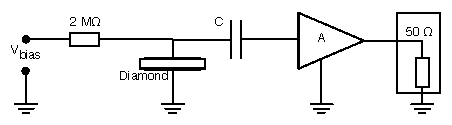
\includegraphics[width=0.7\textwidth]{03_measurement_results/plots/ro-chain}
\caption{Diagram of a diamond detector readout chain.}
\label{fig:ro-chain}
\end{figure}


\subsection{Preamplifiers}
\label{sec:preamps}
Two preamplifiers are used for the measurements. \emph{CIVIDEC Cx} (figure~\ref{fig:ampcx}) is a charge sensitive amplifier. Its high SNR is achieved due to a low equivalent noise charge of 300~e$^-$ with an additional 30~e$^-$ per each pF of the sensor capacitance. A reported gain of $\sim$12~mV/fC makes it a good choice for spectroscopic measurements with diamond sensors. \emph{CIVIDEC C2} (figure~\ref{fig:ampc2})~\cite{1369574} is a fast current preamplifier with a 2~GHz bandwidth limit. %It is used for TCT measurements because of its fast response and a good SNR. 
Both are embedded in an RF-tight aluminium box to reduce the noise pickup. Both have an AC coupled input and a  50~$\Upomega$ output.

A 2~GHz bandwidth limit defines the minimum rising time equal to $t_{\mathrm{r}}\simeq\frac{0.34}{BW}=\frac{0.34}{2\times10^9}=170$~ps. A system with a CIVIDEC C2 amplifier is capable of measuring pulses with a minimum FWHM~$\simeq170~ps$. In practice, this value is for a factor of 3 higher than the rise time, therefore $\sim$500~ps. 

The initial peak in the $\upalpha$ pulse (shown in figure~\ref{fig:drift}) has a lower FWHM; for example, if a positive charge carrier travelling through the bulk takes $t_{\mathrm{1}}\sim~$6~ns to reach the electrode on the opposite side (d$_\mathrm{1}\sim500~\upmu$m), the carrier with the opposite charge and a shorter path to the closer electrode -- max. d$_2\sim10~\upmu$m -- only takes $t_{\mathrm{2}}\sim \frac{d_\mathrm{2}}{d_\mathrm{1}}t_\mathrm{1}\times140~\%=170$~ps (higher percentage due to slower electron drift). Such a short drift time induces a current pulse that is too narrow for the system to detect.


\begin{figure}[!t]
%\centering
\begin{tabular}{cccc}
\subfloat{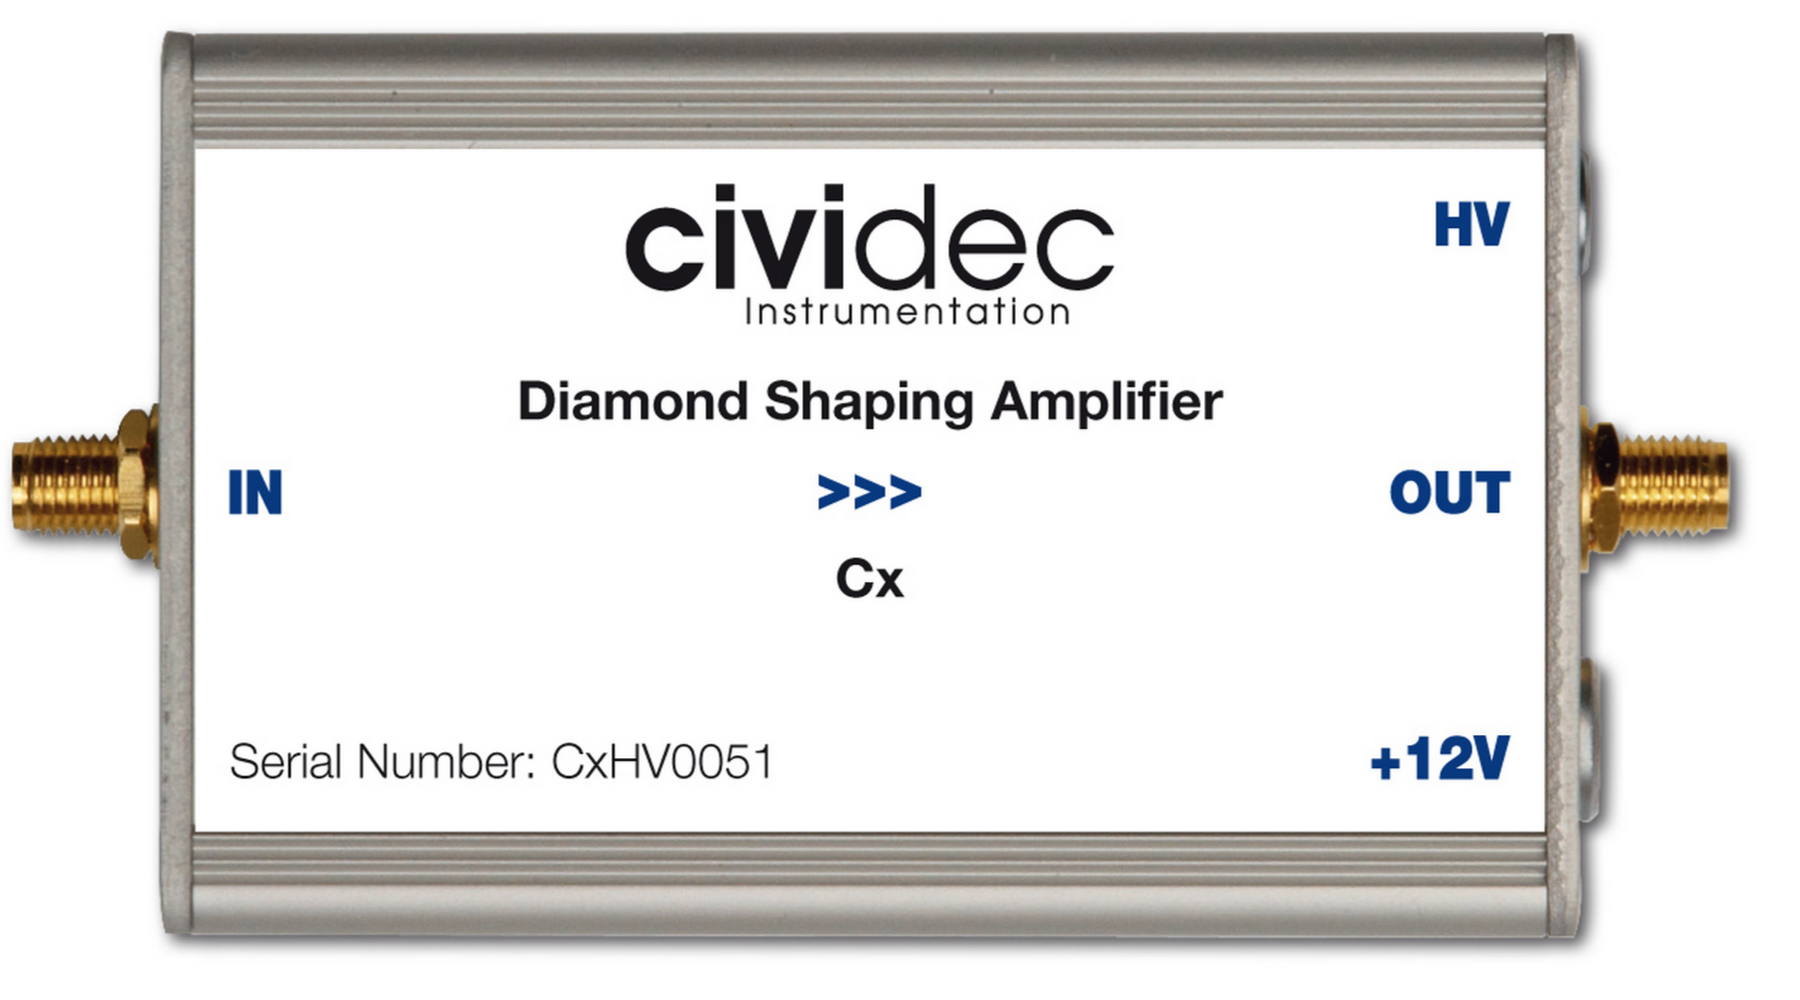
\includegraphics[width=0.47\textwidth]{03_measurement_results/pics/setup/Cx} \label{fig:ampcx}} &
\subfloat{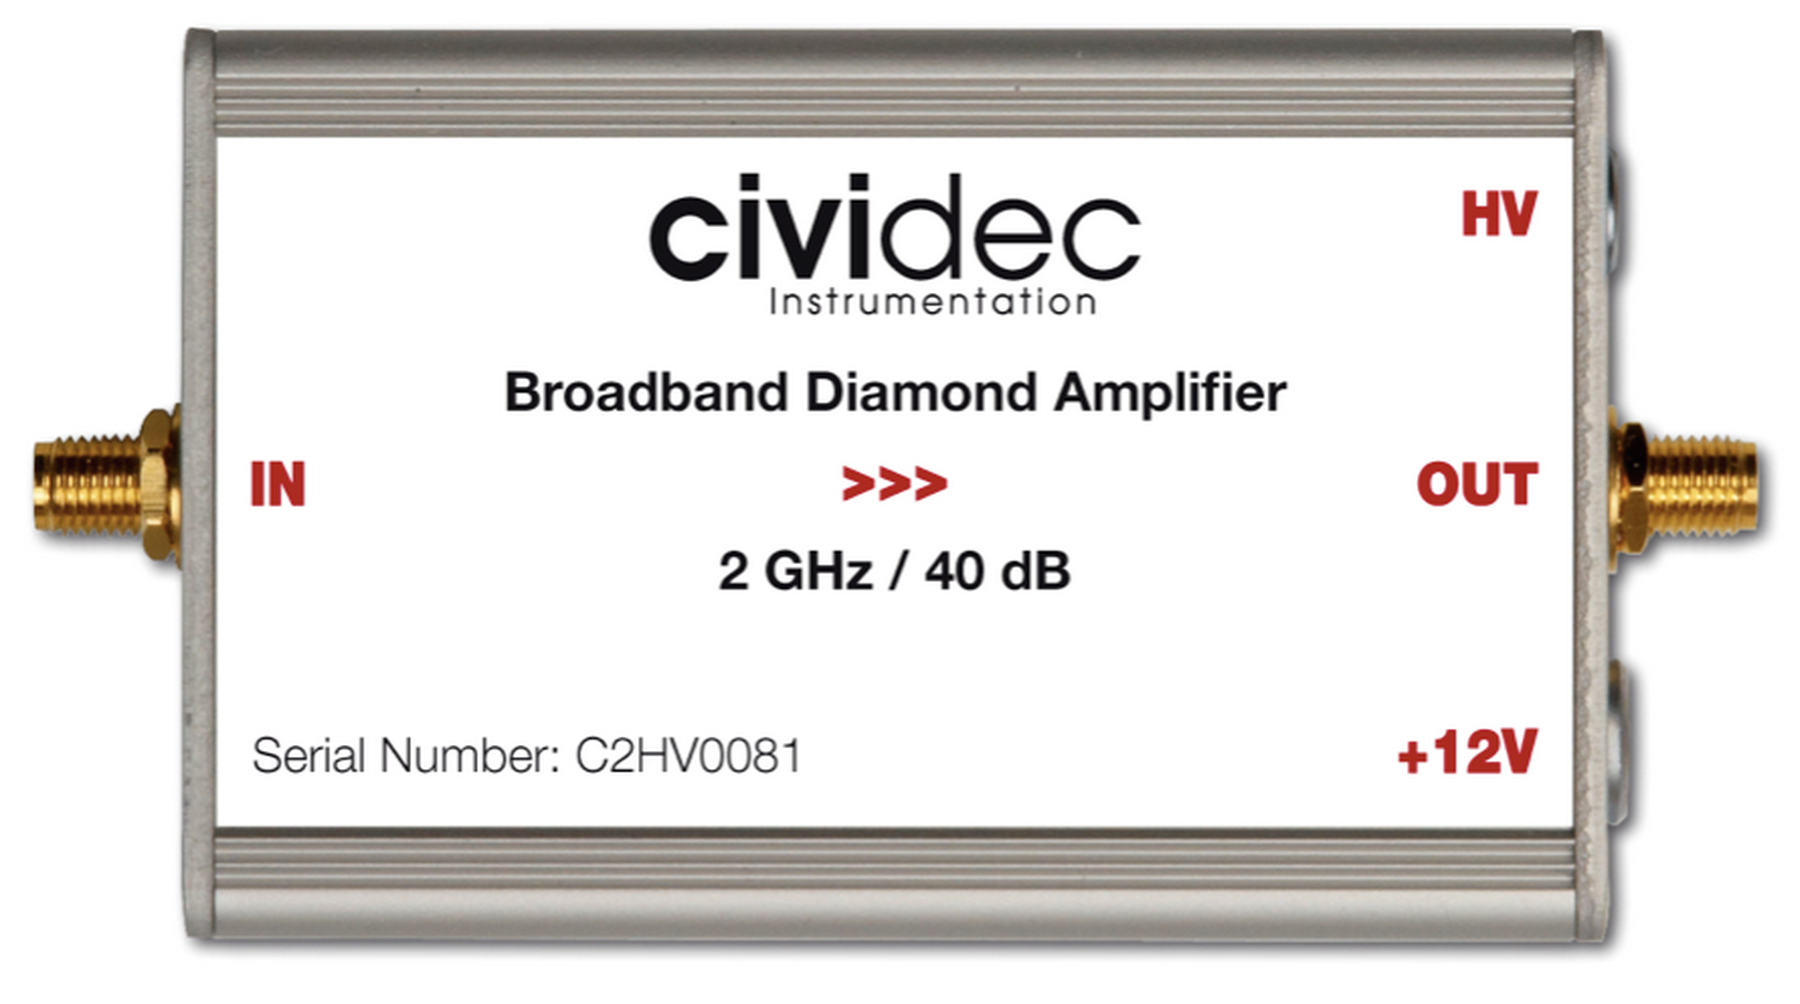
\includegraphics[width=0.47\textwidth]{03_measurement_results/pics/setup/C2}  \label{fig:ampc2}}
\end{tabular}
\caption{CIVIDEC Cx and CIVIDEC C2 amplifiers used for the charge and current measurements.}
\end{figure}


\subsubsection{Calibration}
The amplifiers were calibrated using a square signal generator with a known amplitude step of $U_{\mathrm{in}}=(252\pm5)$~mV. A 2~GHz oscilloscope with a 10~GS/s sampling rate was used to carry out the calibration. 

\begin{description}
\item[Cx charge sensitive amplifier] calibration necessitates an injection of a well known charge. Therefore the signal from a pulse generator is routed through a capacitor with a calibration capacitance $C_{\mathrm{cal}}=(0.717\pm0.014)$~pF and then to the input of the amplifier. The pulse area behind the capacitor is $a_{\mathrm{cal}}=(5.0\pm0.5)$~pVs, with the signal amplitude on the output amounting to $U_{\mathrm{C_x}}=(1.95\pm0.05)$~V. The input voltage step combined with the calibration capacitance yields a calibration charge
\begin{equation}
Q_{\mathrm{cal}}=C_{\mathrm{cal}}\cdot U_{\mathrm{in}}=(181\pm5)~\mathrm{fC}.
\end{equation}
The gain of the Cx amplifier when comparing the integrated input charge to the output amplitude is 
\begin{equation}
A^{\mathrm{Q}}_{\mathrm{Cx}}=\frac{U_{\mathrm{Cx}}}{Q_{\mathrm{cal}} }=(9.3\pm0.4)~\mathrm{mV/fC}
\end{equation}
whereas the factor between the area of the input current pulse and the output amplitude is 
\begin{equation}
A^{\mathrm{a}}_{\mathrm{Cx}}=\frac{U_{\mathrm{Cx}}}{a_{\mathrm{cal}} }=(390\pm40)~\mathrm{mV/pVs}. 
\end{equation}
The area-based amplification factor $A^{\mathrm{a}}_{\mathrm{Cx}}$ can be used as an estimate for the integrated charge of a current pulse. However, it has a higher uncertainty ($\sim10~\%$) than the amplitude-based factor $A^{\mathrm{Q}}_{\mathrm{Cx}}$ ($\sim4~\%$) due to the measurement limitations of the oscilloscope and to RC time constant uncertainty (see figure~\ref{fig:currc}).

\item[C2 current amplifier] calibration only requires the measurement of the amplitude gain. To keep the output signal amplitude within the $\pm1$~V linear range of the amplifier, the input signal amplitude has to be minimised. The signal from the generator is therefore routed through a 36~dB attenuator to decrease its amplitude to $U_{\mathrm{inAtt}}=(3.95\pm0.05)$~mV. Two amplifiers with different gains have been measured, because both are used for the measurements. The output of the first amplifier amounts to $U_{\mathrm{C2-1}}=(860\pm5)$~mV. This yields the amplification gain 
\begin{equation}
A_{\mathrm{C2-1}}=\frac{U_{\mathrm{inAtt}}}{U_{\mathrm{C2-1}}} =(217\pm3). 
\end{equation}
The second amplifier has the output equal to $U_{\mathrm{C2-2}}=(632\pm5)$~mV with the resulting gain of $A_{\mathrm{C2-2}}=(152\pm3)$. 
\end{description}


\subsection{Diamond samples}
\label{sec:diamsam}
%Detector-grade diamonds are very difficult to produce. The major challenge is to ensure a high enough purity of the lattice. %It takes companies years of trials to produce high enough quality product. Since the target market are almost exclusively particle physics research institutes, the companies work closely with them to make sure the product is up to par with the requirements. 
The sCVD diamond sensor samples used for these studies have been acquired from Element Six (E6)~\cite{E6:00000}. They all have the same standard dimensions of $4.7\times4.7$~mm$^2$. % are already sufficiently large for most of the beam monitoring applications and still affordable. 
%; the cost of sCVD diamonds grows exponentially with the area. There is also an ongoing race among the producers to produce larger and larger diamonds while maintaining the same cost. For instance, a new company IIa~\cite{} from Singapore has produced high-quality samples with larger dimensions and the diamond detector community is currently involved in extensive tests of their products. 
One sample with dimensions of $5.6\times5.3$~mm$^2$ produced by IIa Singapore~\cite{IIA:00000} has also been characterised at CERN~\cite{IIa:00001}. The target thickness for all samples is 500~$\upmu$m. %Diamonds this thick yield a high enough signal-to-noise ratio for MIPs to be measured by the available electronics.
\begin{figure}
\centering
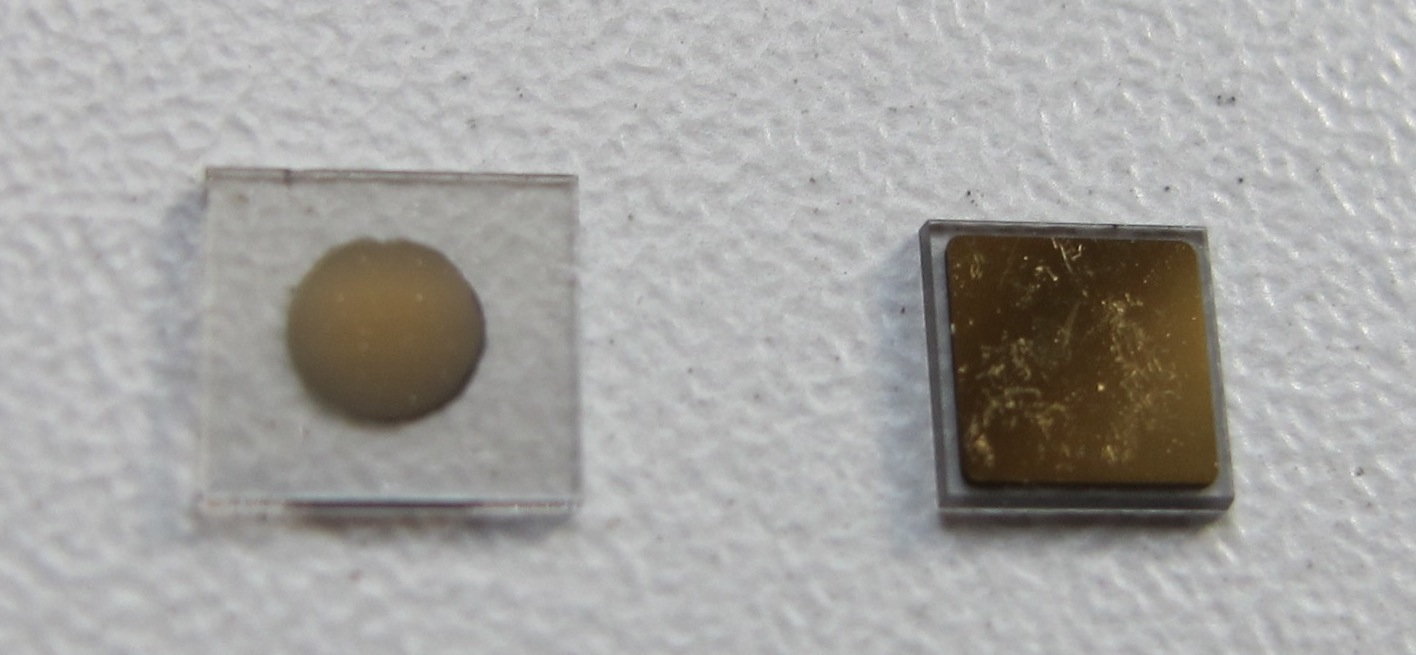
\includegraphics[width=0.7\textwidth]{03_measurement_results/pics/setup/diamond4}
\caption{Two scCVD diamond samples: A IIa 1scdhq (left) and an E6 S37 (right).}
\label{fig:diams}
\end{figure}
Table~\ref{tab:diamsamp} shows all diamond samples used for this study. Two of them are measured before and after irradiation and then compared. %Irradiation doses for damaging the material need to be high -- above $10^{12}$~particles per cm$^2$ to be able to observe a significant change in behaviour of a diamond sensor. 

\begin{footnotesize}
\begin{center}
\begin{tabular}{   l  c  c  c  c c c }
\hline
Name & Type &Producer & Dimensions [mm$^2$] & Thickness [$\upmu$m] & Electrode & Irradiated \\
\hline
S37 & sCVD & E6 & $4.7\times4.7$ & 548 & Cr/Au & no \\
S50 & sCVD & E6 & $4.7\times4.7$ & 537 & Cr/Au & no \\
S52 & sCVD & DDL & $4.7\times4.7$ & 515 & DLC/Pt/Au & $3.6\times10^{14}~\frac{\uppi}{cm^{2}}$ \\
S79 & sCVD & E6 & $4.7\times4.7$ & 529 & Cr/Au & $1\times10^{14}~\frac{\uppi}{cm^{2}}$ \\
ELSC & sCVD & E6 & $4.7\times4.7$ & 491 & Cr/Au & no \\
1scdhq & sCVD & IIa & $5.6\times5.3$ & 460 & Cr/Au & no \\
\hline
\end{tabular}
\captionof{table}{Diamond sensor samples used.}
\label{tab:diamsamp}
\end{center}
\end{footnotesize}
%_\mathrm{300~MeV}

The diamond samples have quoted impurity densities of $\leq2\times10^{14}$~cm$^{-3}$ and nitrogen incorporation of $\leq10^{-9}$~\cite{Jansen:1956431}. The electrodes were added by various companies and institutes. For instance, S52 was metallised by a company DDL (now defunct) while the Physics Department of the University of Firenze, Italy metallised the S79. There are also several techniques for producing the electrodes. The DDL contacts consist of three layers: DLC (diamond-like carbon)/Pt/Au with 4/10/200 nm thicknesses, respectively. The metallisation for S79, on the other hand, is made up of Cr/Au with a total thickness of $\sim$400~nm. The area coverage also differs from sample to sample. Diamonds must not be metallised until the very edge as the proximity of contacts with a high potential difference may lead to bias voltage shorts on sensor edges. However, the areas not covered by the metallisation are less efficient because the fringe fields at the edges are not as strong as in between the electrodes. This effectively reduces the sensitive area of the sensors. In the diamonds used here the effective area is anywhere from 9~mm$^2$ to 18~mm$^2$. The leakage current is below 1~nA, but increases for the irradiated samples. The capacitance is of the order of (2.0$\pm$0.3)~pF for 1scdhq.


\subsection{Readout devices}
\label{sec:readoutdev}
Electrical signals in diamond detectors are in the GHz frequency range. To preserve the information in the signals, the readout device with a high bandwidth limit must be used. For instance, a 20~MHz limit is enough for the spectroscopic measurements with the Cx charge amplifier, but is insufficient for the current measurements with the C2 amplifier. 

Two devices are used take data shown in this chapter. The first choice is a 2~GHz LeCroy WaveRunner 204MXi-A. This specific model has a sufficiently high bandwidth limit for the fast current preamplifier signals. It offers a reliable solution for analogue signal readout of limited amounts of data. 
%However, its slow acquisition speed is a bottleneck in a test beam experiment. Its initial 100~Hz readout rate decreases to a mere 20~Hz within 20 minutes, because every single trigger is saved as a separate file and the Windows operating system is not capable of handling $10'000$+ files in a single directory easily. 
The second device is DRS4~\cite{DRS4:00000}, an analogue data acquisition device developed by PSI, Switzerland, capable of recording up to four waveforms at a time at a steady rate of up to 500~Hz. Its 700~MHz bandwidth limitation is sufficient for the signal from the charge and the current amplifier.



\subsection{Setup for the $\upbeta$ detection efficiency study}
A charge collection efficiency study of the diamond sensors has been carried out at CERN in the North Hall test beam facility. There a straight high-energy particle beam of 120~GeV/c~$\uppi$ is provided to the users to calibrate their detectors. The beam has a transverse spread of $\sigma=10$~mm in both axes. The particle rate is of the order of $10^4~\uppi$~cm$^{-2}$~s$^{-1}$. A diamond sensor embedded in a printed circuit board (PCB) carrier has been placed in the beam spot perpendicular to the beam and connected via an SMA connector directly to a charge sensitive amplifier. The amplified signal is read out using a LeCroy oscilloscope and a DRS4 analogue readout system. A computer is used as a controller and data storage for the readout device. A beam telescope is used as a reference detector. It is a device that helps to cross-check the measurements of the devices under test (DUTs) and to carry out spatially resolved studies on the DUTs. It consists of several pixellated sensor planes, such as FE-I4~\ref{1748-0221-7-11-P11010}, placed in series, which can track a particle's trajectory with a precision of a few $\upmu$m. The sensor planes are positioned in front of the DUT and behind it. Then the beam telescope acts as a trigger system -- it triggers the readout of both the telescope data and DUT data when both the planes in front and behind the DUT record a hit by an incident particle. A particle detected by all the planes within the DUT window and the DUT itself counts towards its efficiency whereas a hit missed by the DUT means that the DUT is not 100~\% efficient. To discard the hits that miss the DUT completely, a region of interest (ROI) can be chosen in the beam telescope planes. The equation for calculating the sensor efficiency is therefore
\begin{equation}
\label{eq:sensoreff}
\epsilon = \frac{ N_\mathrm{DUT} \wedge N_\mathrm{telescope} }{ N_\mathrm{telescope} }
\end{equation}
for an ROI smaller than the sensitive region of the diamond.


\subsection{Room temperature $\upalpha$-TCT setup}
Room-temperature TCT measurements have been carried out in the laboratory. The setup consists of a diamond sensor embedded in a PCB carrier, a current amplifier and an oscilloscope. To measure $\upalpha$ particles, their energy loss during their trajectory has to be minimised. Therefore the diamond is placed inside a vacuum chamber to avoid energy loss in air. The chamber is a steel tube with a diameter of 5~cm. On one side it is connected to a vacuum pump via a steel hose. A feedthrough with an SMA connector is placed on the other side. A CIVIDEC C2 current amplifier is connected directly onto the feedthrough. The amplified output is connected to the oscilloscope via an SMA cable. An $^{241}$Am source with a diameter of 2~cm and a height of 0.5~cm is fixed onto the sensor carrier (figure~\ref{fig:carrier}, figure~\ref{fig:carsrc}). Then the carrier is inserted in the chamber and fixed in place using an air-tight clamp. The pump can then be switched on. It is capable of providing an inside pressure as low as $10^{-4}$~mbar after approximately one hour of operation.
%on Malte's instructions I'm leaving this out.
%, but measurements can take place even after five minutes of evacuation, at around $10^{-3}$~mbar. The most important thing is to switch the bias voltage of the sensor OFF during the process of evacuation. This is due to gas becoming more conductive at the pressure of the order of $10^{-1}$~mbar, which is at the bottom of Paschen's curve~\cite{PASCHEN:00000}. A failure to switch the bias voltage off may cause a spark between the signal and ground line, destroying the amplifier. 

\begin{figure}[!t]
%\centering
\begin{tabular}{cccc}
\subfloat{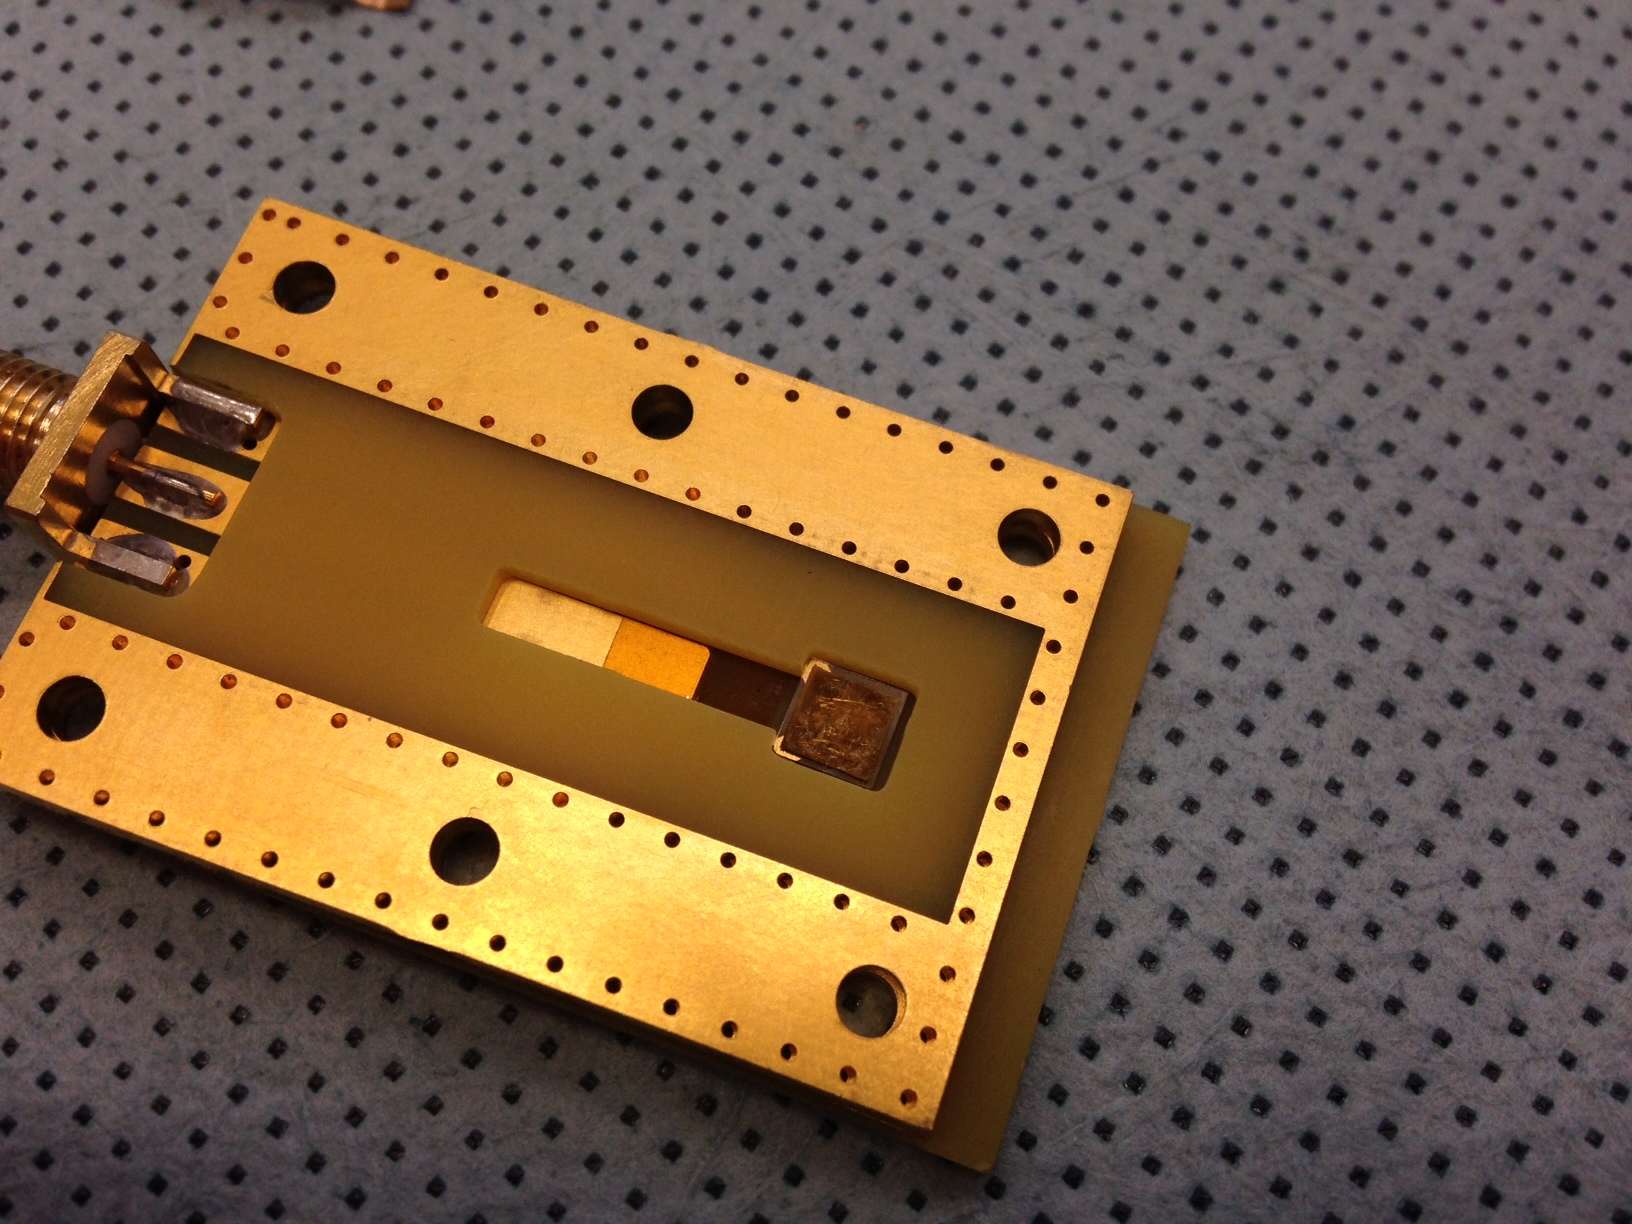
\includegraphics[width=0.47\textwidth]{03_measurement_results/pics/setup/carrier2} \label{fig:carrier}} &
\subfloat{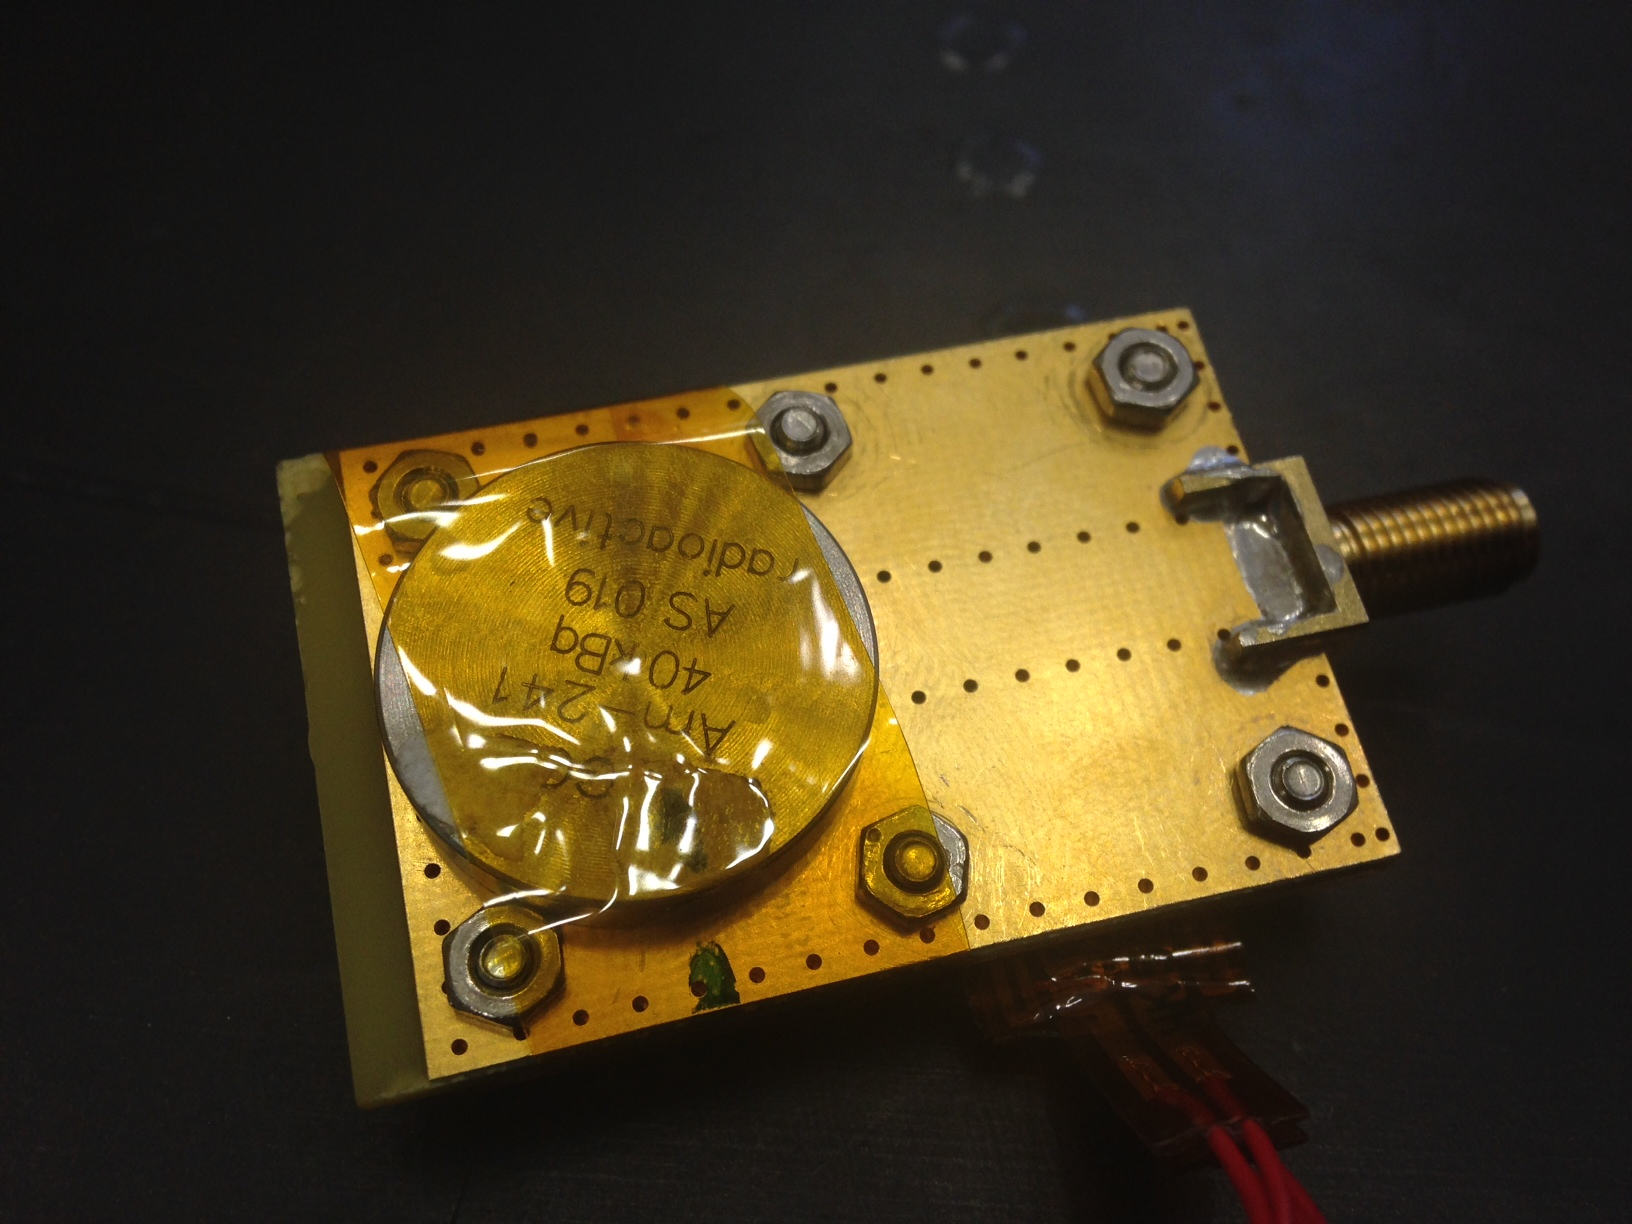
\includegraphics[width=0.47\textwidth]{03_measurement_results/pics/setup/carriersource2}  \label{fig:carsrc}}
\end{tabular}
\caption{Positioning of the $\upalpha$-source on top of the sensor carrier.}
\end{figure}


\subsection{Cryogenic $\upalpha$-TCT setup}
\label{sec:cryosetup}
This TCT study is a follow-up of an extensive diamond TCT study at cryogenic temperatures~\cite{Jansen:1956431}. The experiment at cryogenic temperatures has been carried out at the Central Cryogenic Laboratory at CERN. The room-temperature TCT setup has to be modified to allow for measurements at temperatures as low as 4~K. It consists of three parts: 
\begin{enumerate}
\item a cryostat --  a thermally insulated cylinder containing liquid helium,
\item an inlet -- an air-tight mechanical tube with valves and feedthroughs at the top that is lowered in the liquid helium and
\item a diamond sample embedded in a PCB carrier with a fitted temperature sensor, a heater and cables leading to the feedthroughs.
\end{enumerate}
The setup is described in detail in~\cite{Jansen:1956431}.

When the diamond sample is placed in the PCB carrier and the $^{241}$Am $\upalpha$ source is in place, the inlet is sealed and lowered in the empty cryostat. Then the inside volume of the inlet is evacuated down to $10^{-5}$~mbar while the liquid helium is flowing into the cryostat. To improve the thermal contact between the diamond and the coolant, a small amount of helium gas is added inside the evacuated inlet, setting the vacuum to around $10^{-3}$~mbar. This value changes with time, because the gas condenses on the walls of the inlet, reducing the number of floating particles. For this reason the helium gas has to be added on a regular basis. Every addition causes a significant undershoot of the sample temperature, which has to be corrected for using a heater placed on the back of the PCB carrier. Also, the added gas deteriorates the vacuum inside the inlet. 
%deleted on Malte's instructions
%It is very important to monitor the pressure so as not to let it rise above $10^{-2}$~mbar. The gas at this pressure is significantly more conductive and can cause a short circuit between the two diamond plates or in the SMA connectors, destroying the amplifier. 
Furthermore, at approximately 60~K the helium gas has to be evacuated from the inlet to avoid a potential explosion due to the expansion of the gas with temperature. 

When the sample is cooled to 4~K, the minimum temperature achievable by means of liquid helium without over-pressurising it, the measurements can begin. A temperature sensor placed on the back of the PCB carrier is used to measure the temperature of the sample. After every measurement, the current through the heater is increased, heating up the sample to the next temperature point. The initial temperature time constant of the order of tenths of seconds at low temperatures increases with temperature. Even more so when helium is evacuated from the inlet at 60~K, removing the thermal bridge between the wall of the inlet and the diamond sample. At the room temperature (RT), the time constant is already of the order of minutes.

% ---------------------------------------------------------------------------------------------------------------
%\clearpage
\section{Charged particle pulses and spectra}
\label{sec:pulsespectra}
% ---------------------------------------------------------------------------------------------------------------
In previous chapter the ionisation profiles for different types of radiation were discussed. A $\upbeta$ particle induces a triangular electric pulse whereas a pulse induced by an $\upalpha$ particle is rectangular. However, their amplitude, width and rise/fall time depend heavily on the type of interaction with the diamond, the purity of the diamond and the bandwidth of the amplifier and the oscilloscope. This section shows the signal pulses of $\upalpha, \upbeta$ and $\upgamma$ radiation with their respective energy distributions for the case of a diamond detector. %This is followed by a discussion of effects of noise on these measurements. 

Figure~\ref{fig:pulsesaby} shows a set of pulses and an averaged waveform for 5.5~MeV $\upalpha$, 2.3~MeV $\upbeta$ and 1.3~MeV $\upgamma$ radiation using an $^{241}$Am, a $^{90}$Sr and a $^{60}$Co source, respectively. The particles are measured with the non-irradiated sCVD diamond S37. $\upalpha$ particles always produce the same signal pulse with a noise RMS of 2.7~mV. The averaging suppresses the noise while retaining most the information. It does, however, smear the rising and falling edge, increasing the rising and falling time. The $t_{\mathrm{r}}$ is now of the order of 0.5~ns. The pulse count for $\upbeta$ and $\upgamma$ is low, so the pulses with a high amplitude are not recorded. A trigger would need to be set very high to ``catch'' them with the oscilloscope. Both $\upbeta$ and $\upgamma$ pulses look similar - triangular and with a wide range of amplitudes.

Histograms on the right hand side of figure~\ref{fig:pulsesaby} show distributions for of deposited charge as measured with a CIVIDEC Cx amplifier. The distribution of $\upalpha$ particles is a Gaussian function. The $\upbeta$ distribution follows a Landau function. This is due to scattering of $\upbeta$ in the sensor. Some $\upbeta$ maintain a straight trajectory while traversing the sensor. Those create a Gaussian-like distribution. Others scatter in the lattice, extending the effective length of the path and therefore increasing the number of excited e-h pairs. In some cases the $\upbeta$ produce a shower of secondary particles, which in turn create more e-h pairs. Contributions from all types of interactions form a Landau distribution.

$\upgamma$ distribution on the other hand is expected to be a convolution of signals created by photoelectric and Compton interactions. The expected distribution is an exponential. The acquired data are taken with a self-trigger set to 20~mV to minimise noise contribution. %Therefore the distribution includes signals from scattered particles and noise contributions.

\begin{figure}[!t]
\centering
\begin{tabular}{rrr}
\subfloat{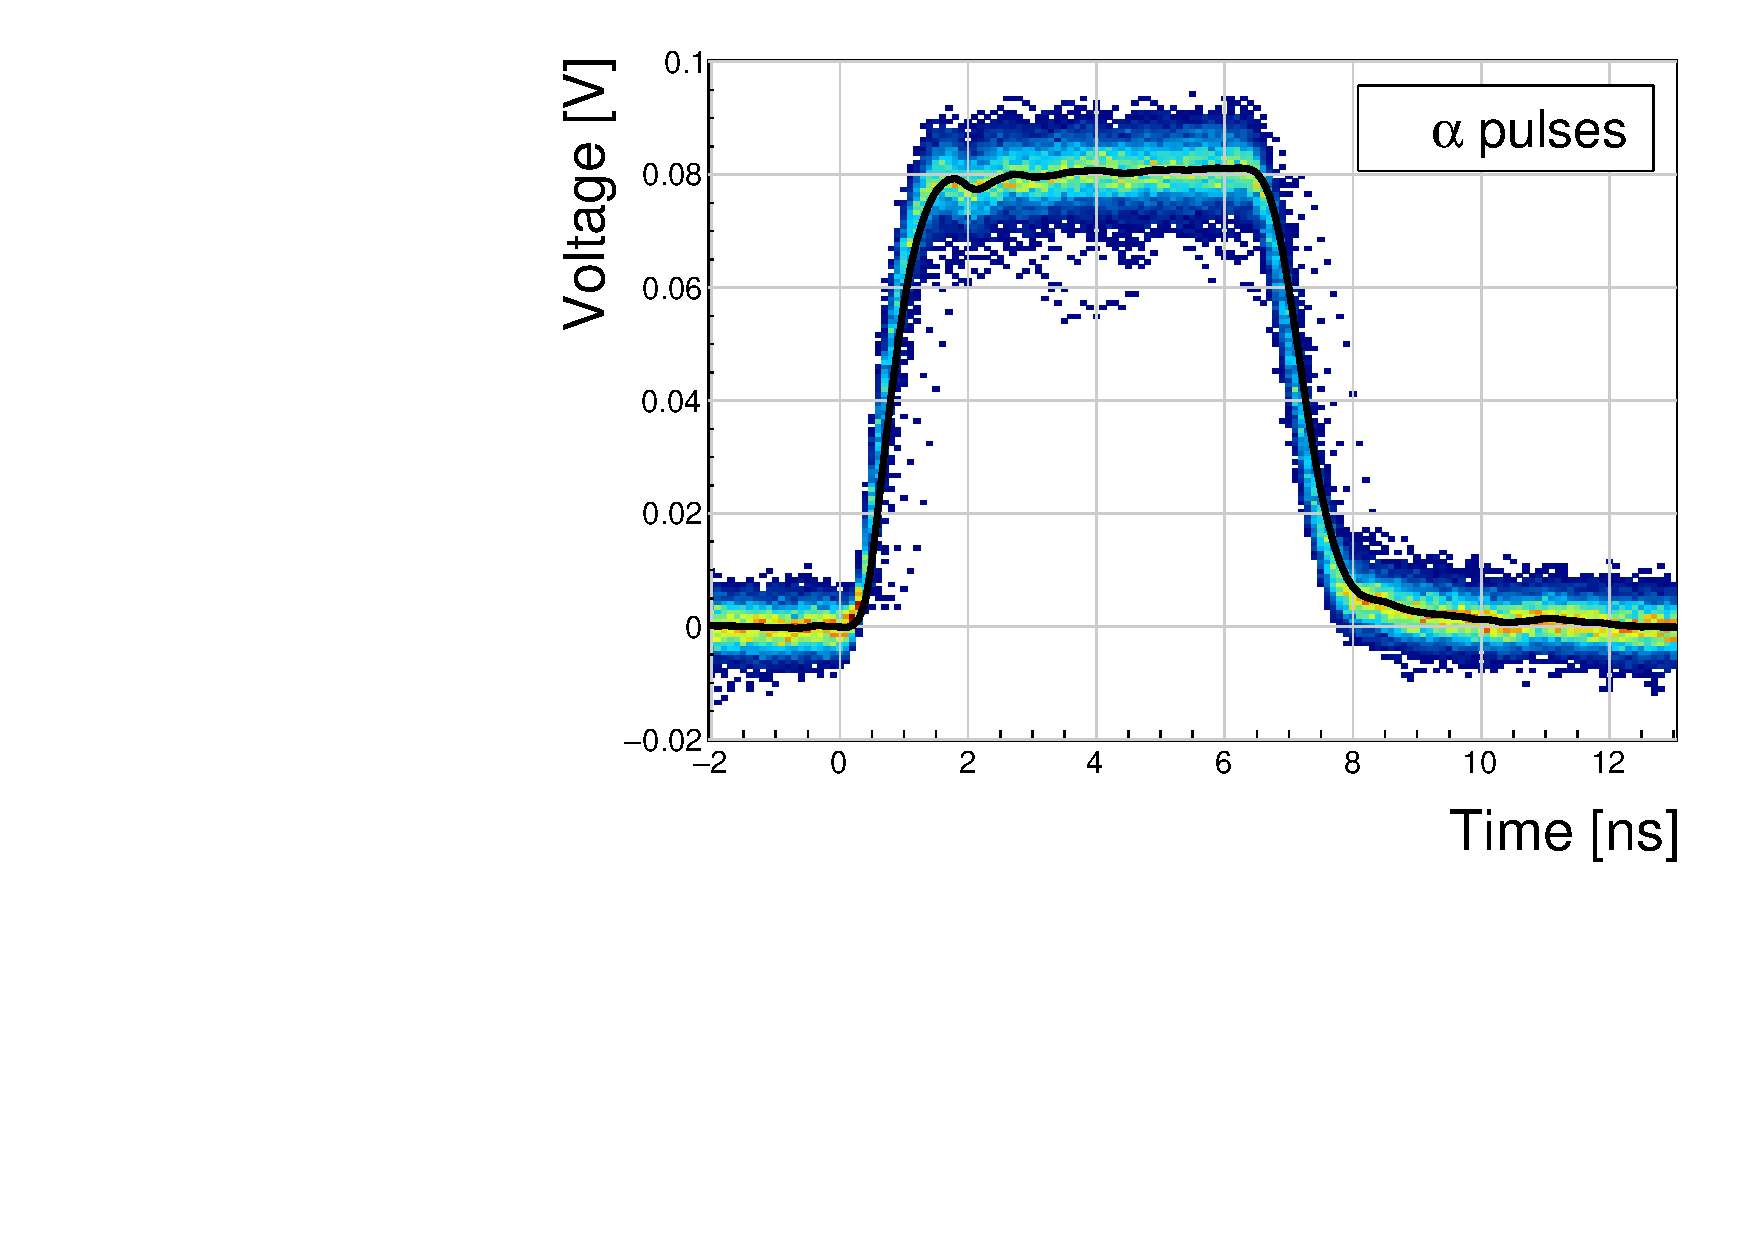
\includegraphics[width=0.47\textwidth]{03_measurement_results/scripts/plots/samplePulses/alpha} \label{fig:alpha1}} &
\subfloat{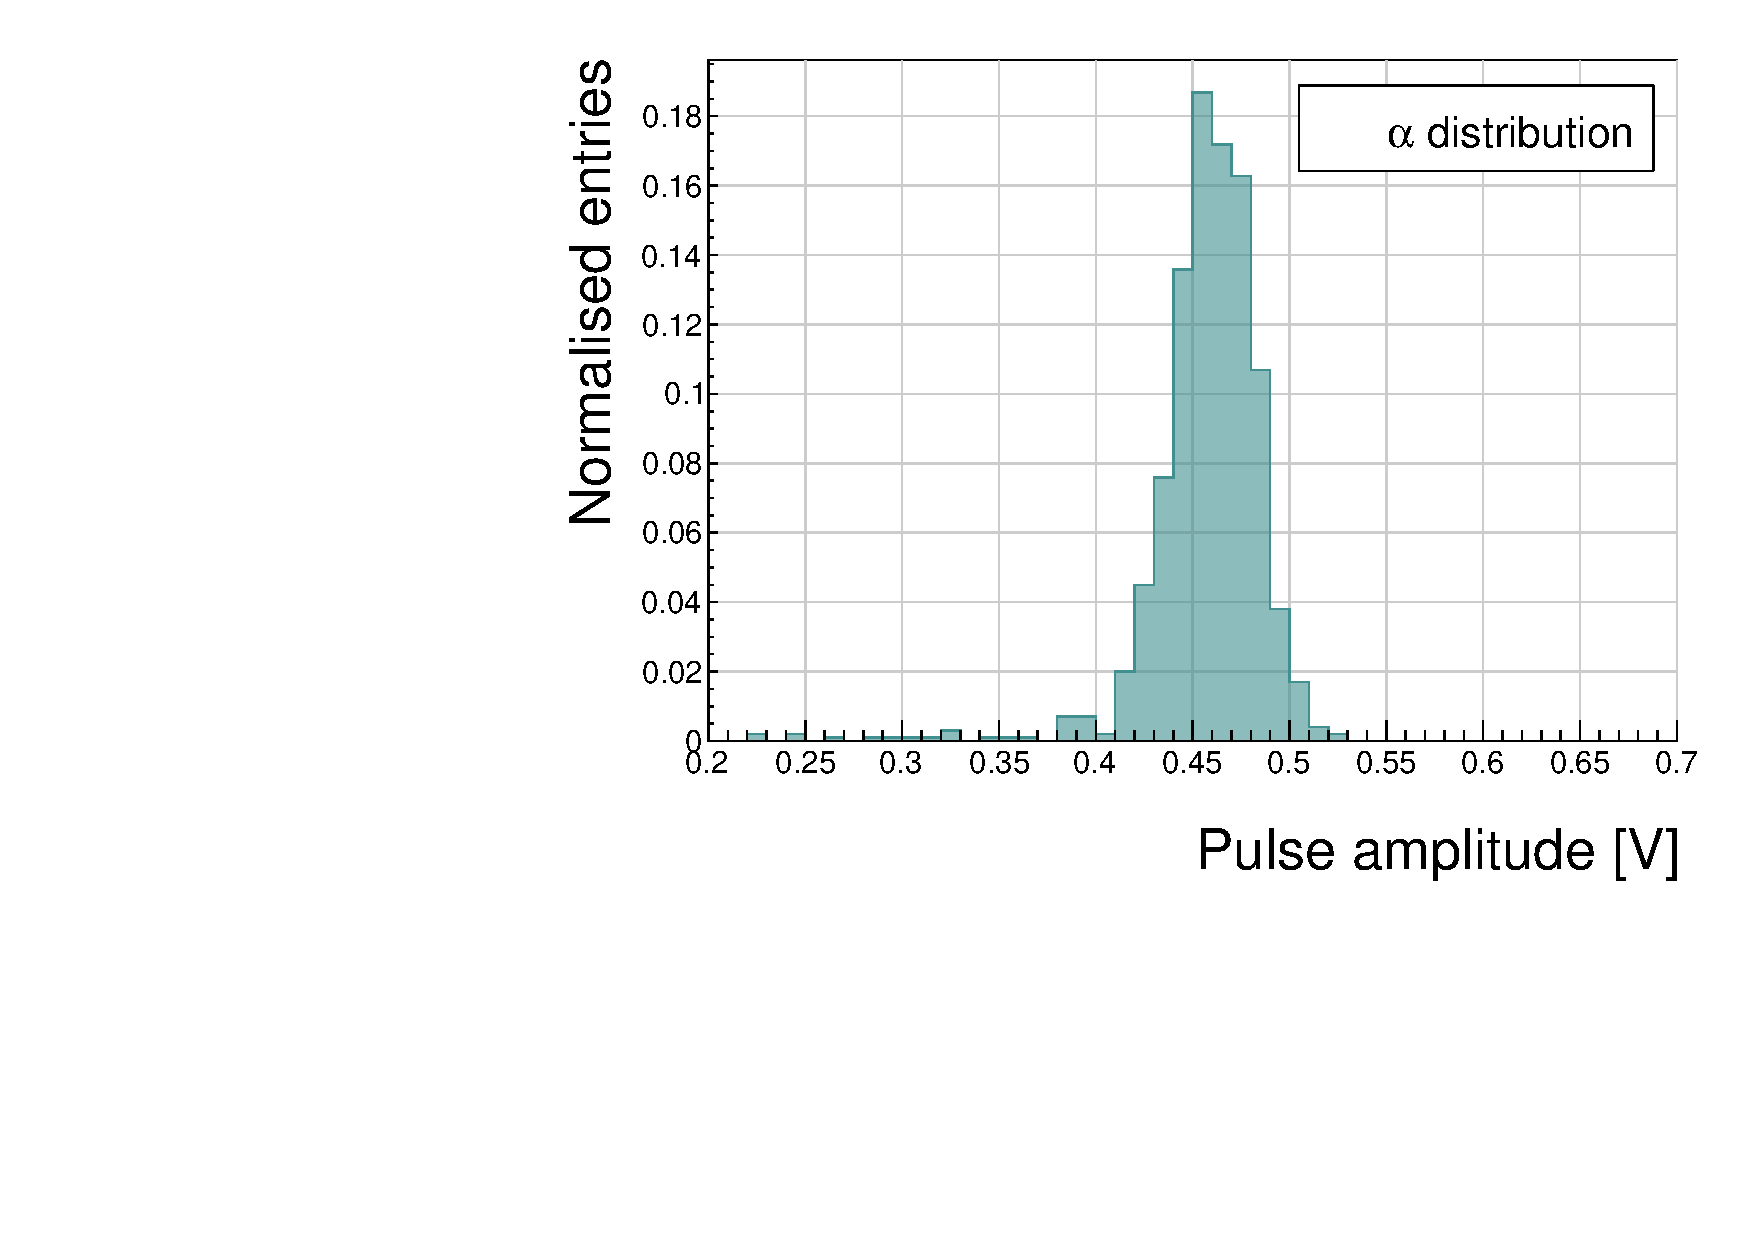
\includegraphics[width=0.47\textwidth]{03_measurement_results/scripts/plots/samplePulses/alphadist} \label{fig:alphadist1}} \\
\subfloat{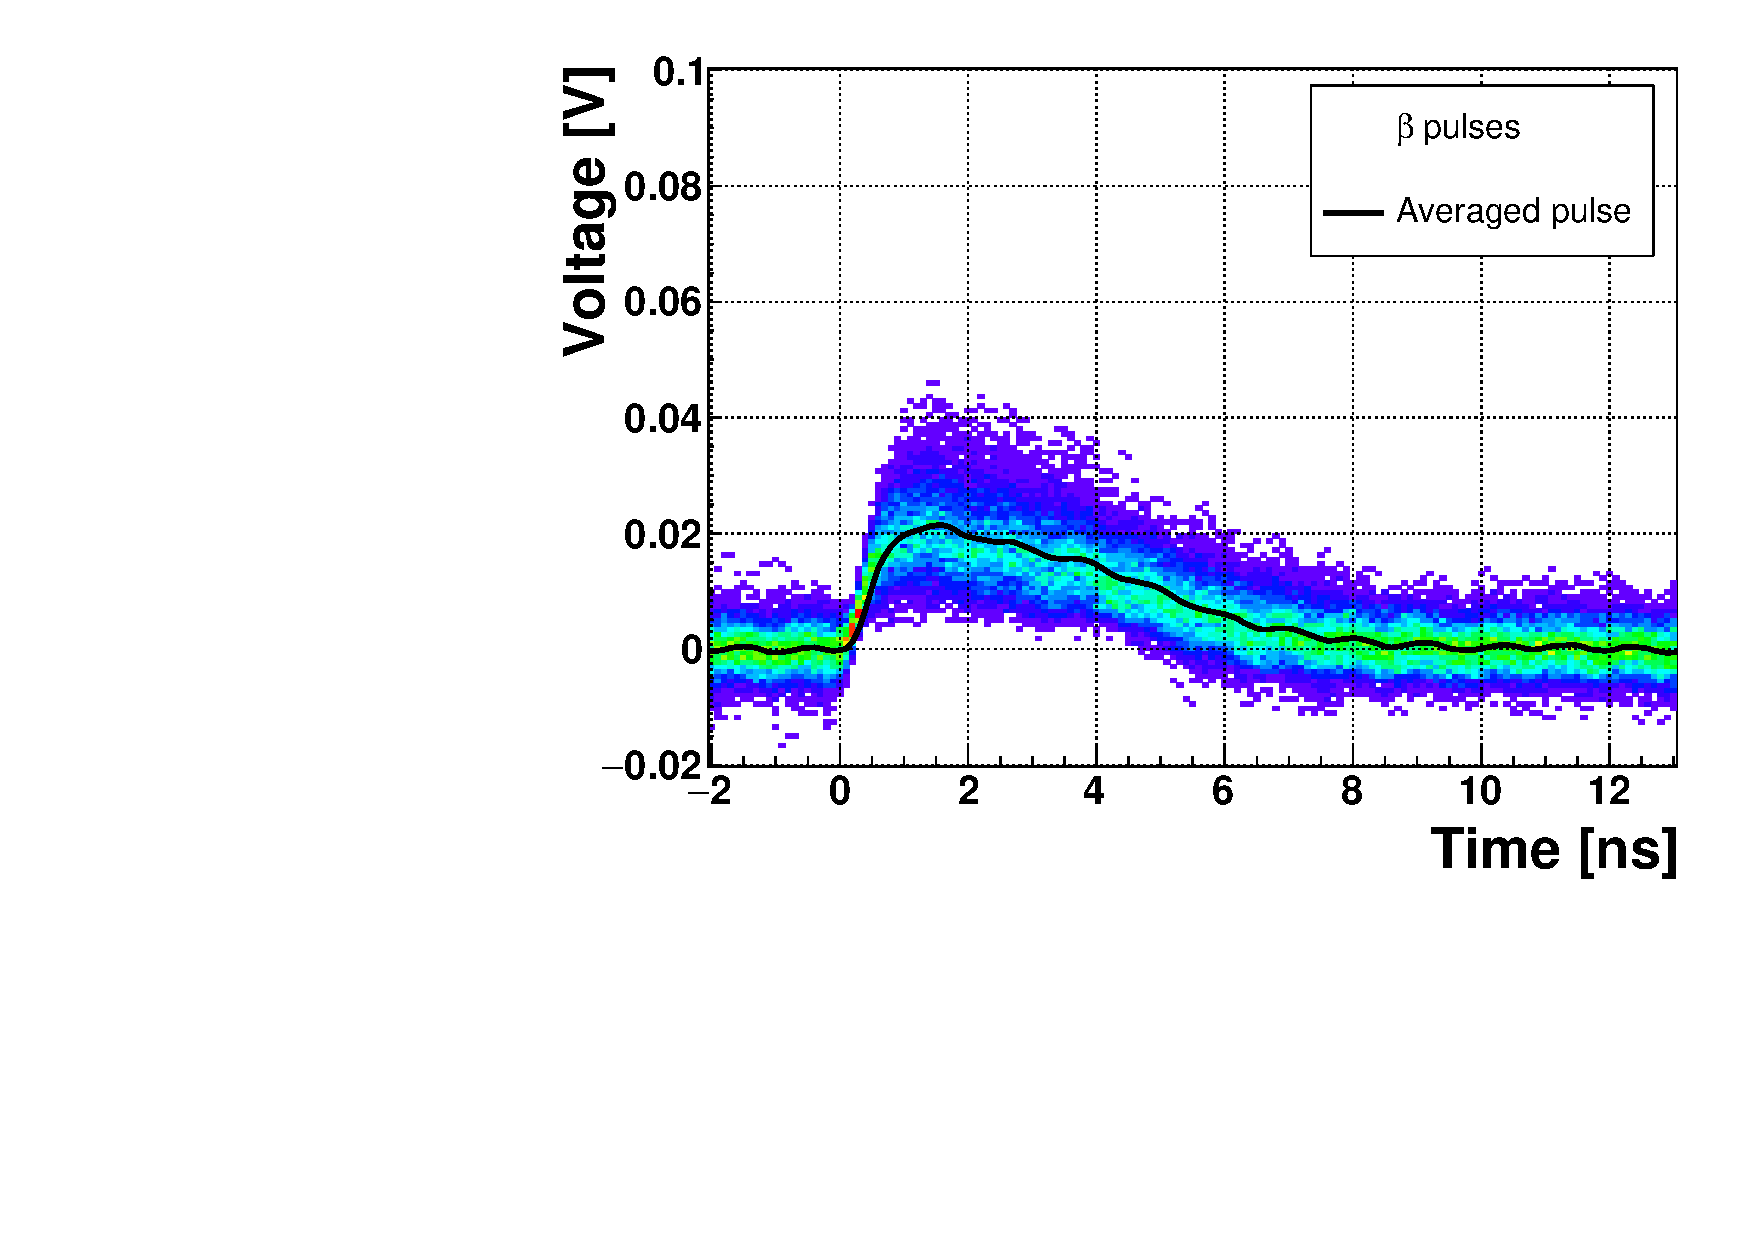
\includegraphics[width=0.47\textwidth]{03_measurement_results/scripts/plots/samplePulses/beta}  \label{fig:beta1}} &
\subfloat{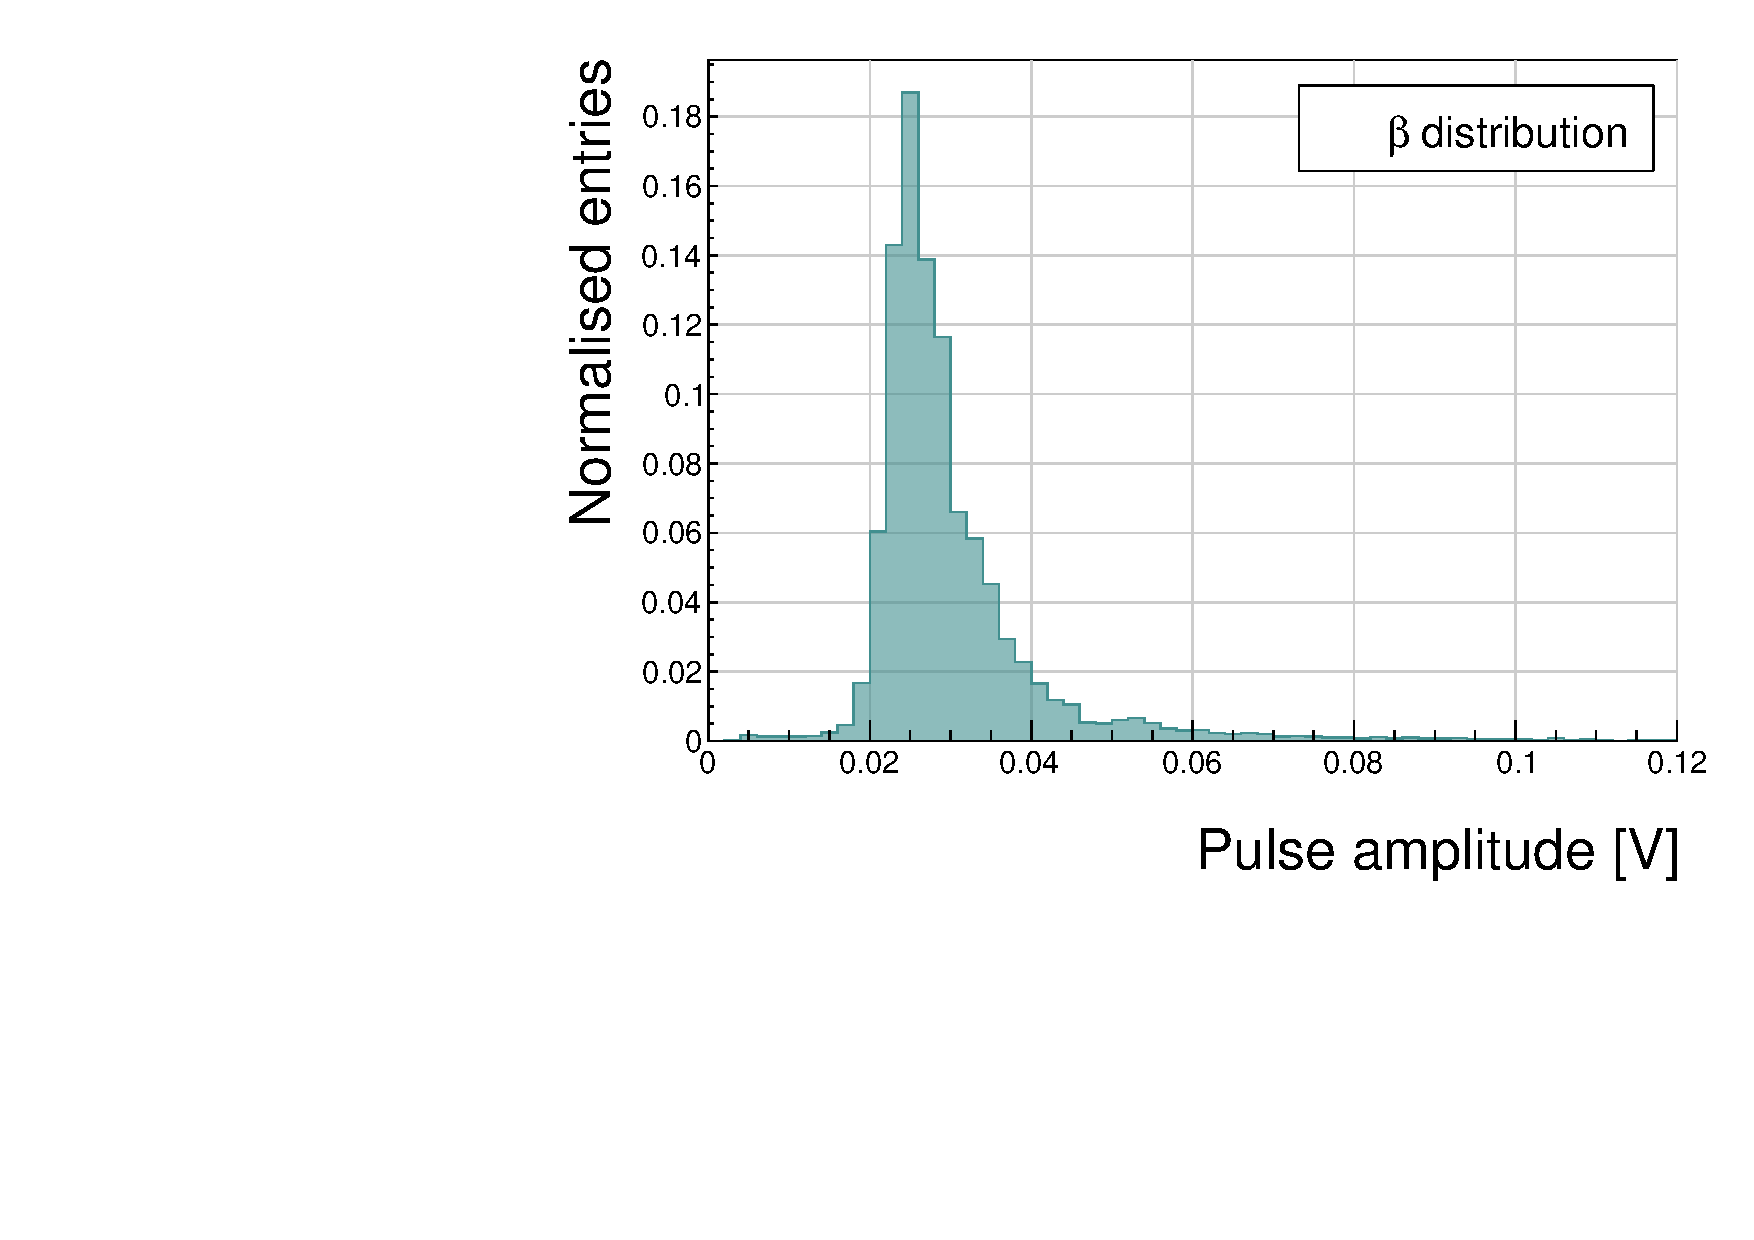
\includegraphics[width=0.47\textwidth]{03_measurement_results/scripts/plots/samplePulses/betadist}  \label{fig:betadist1}} \\
\subfloat{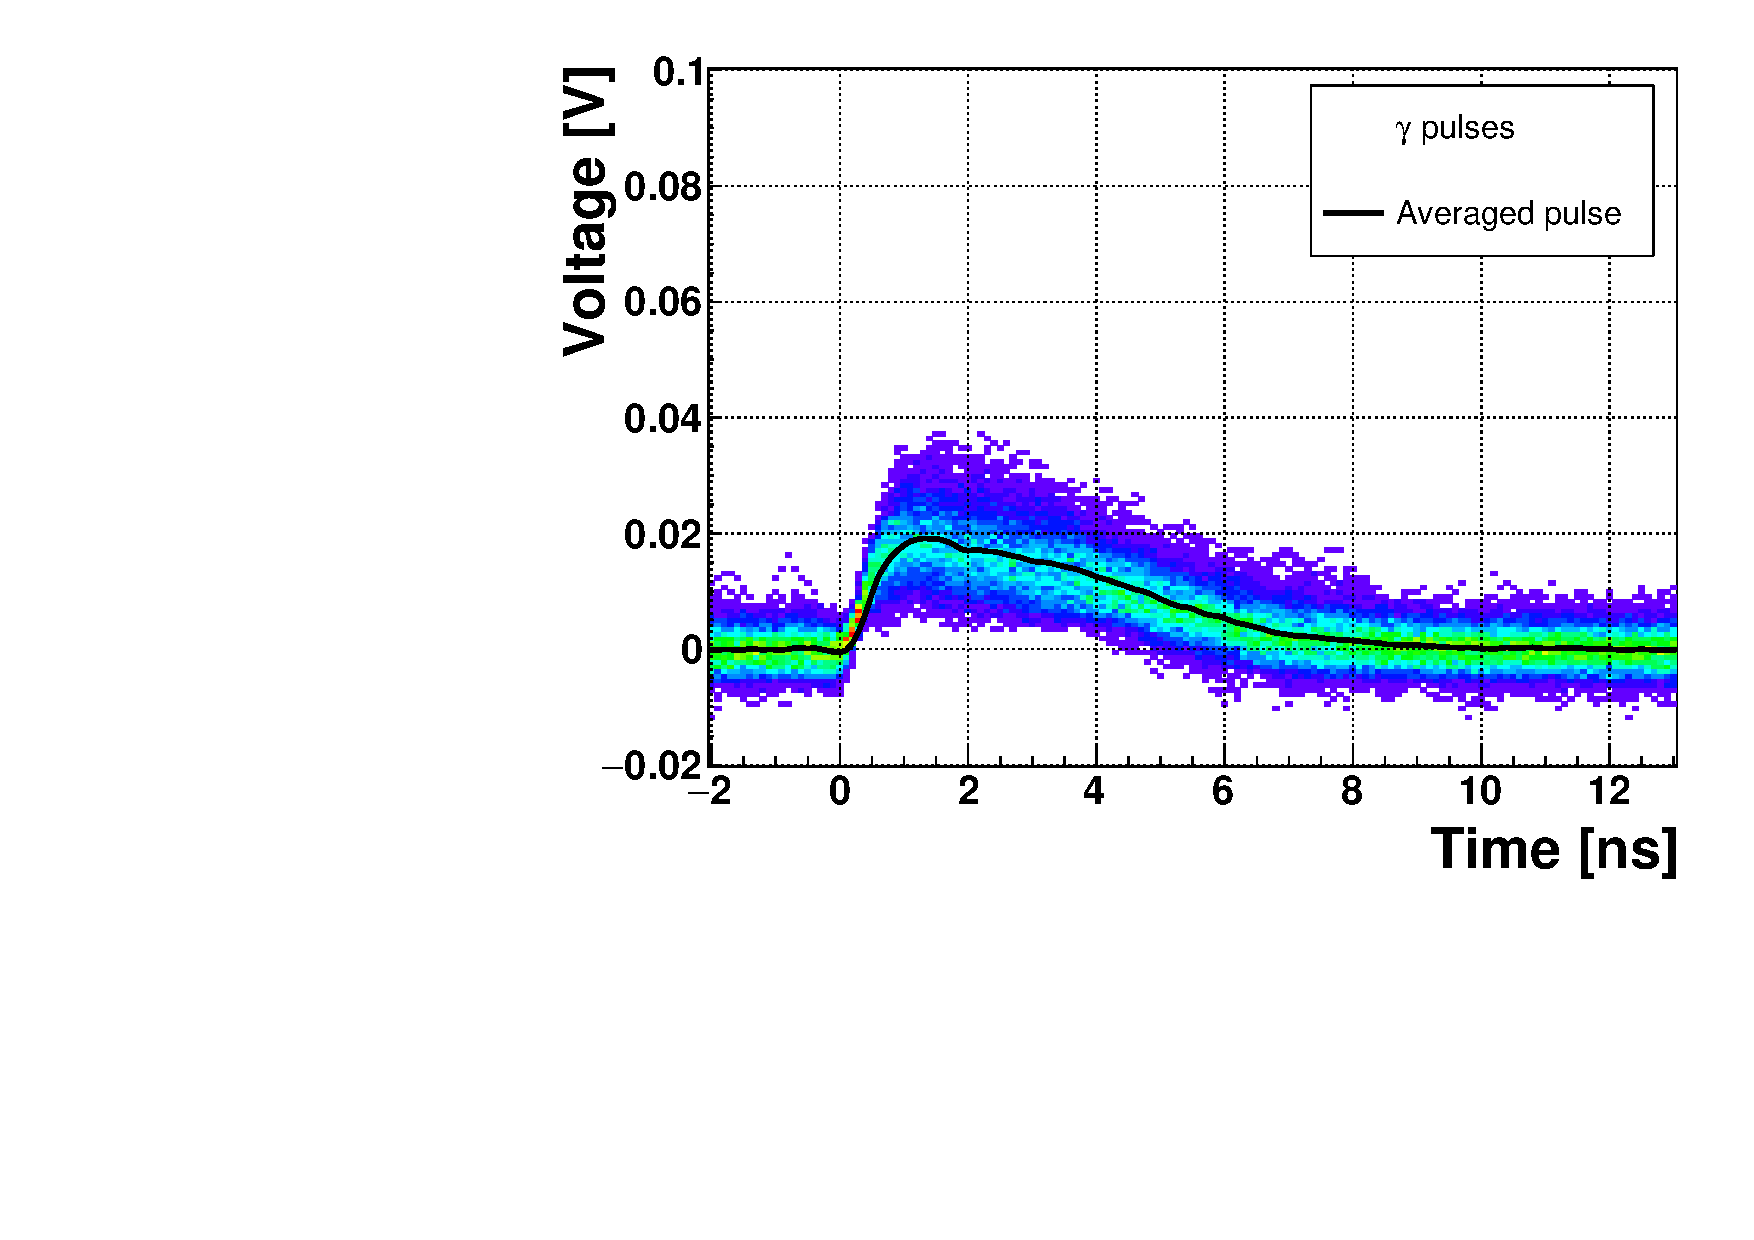
\includegraphics[width=0.47\textwidth]{03_measurement_results/scripts/plots/samplePulses/gamma}  \label{fig:gamma1}} &
\subfloat{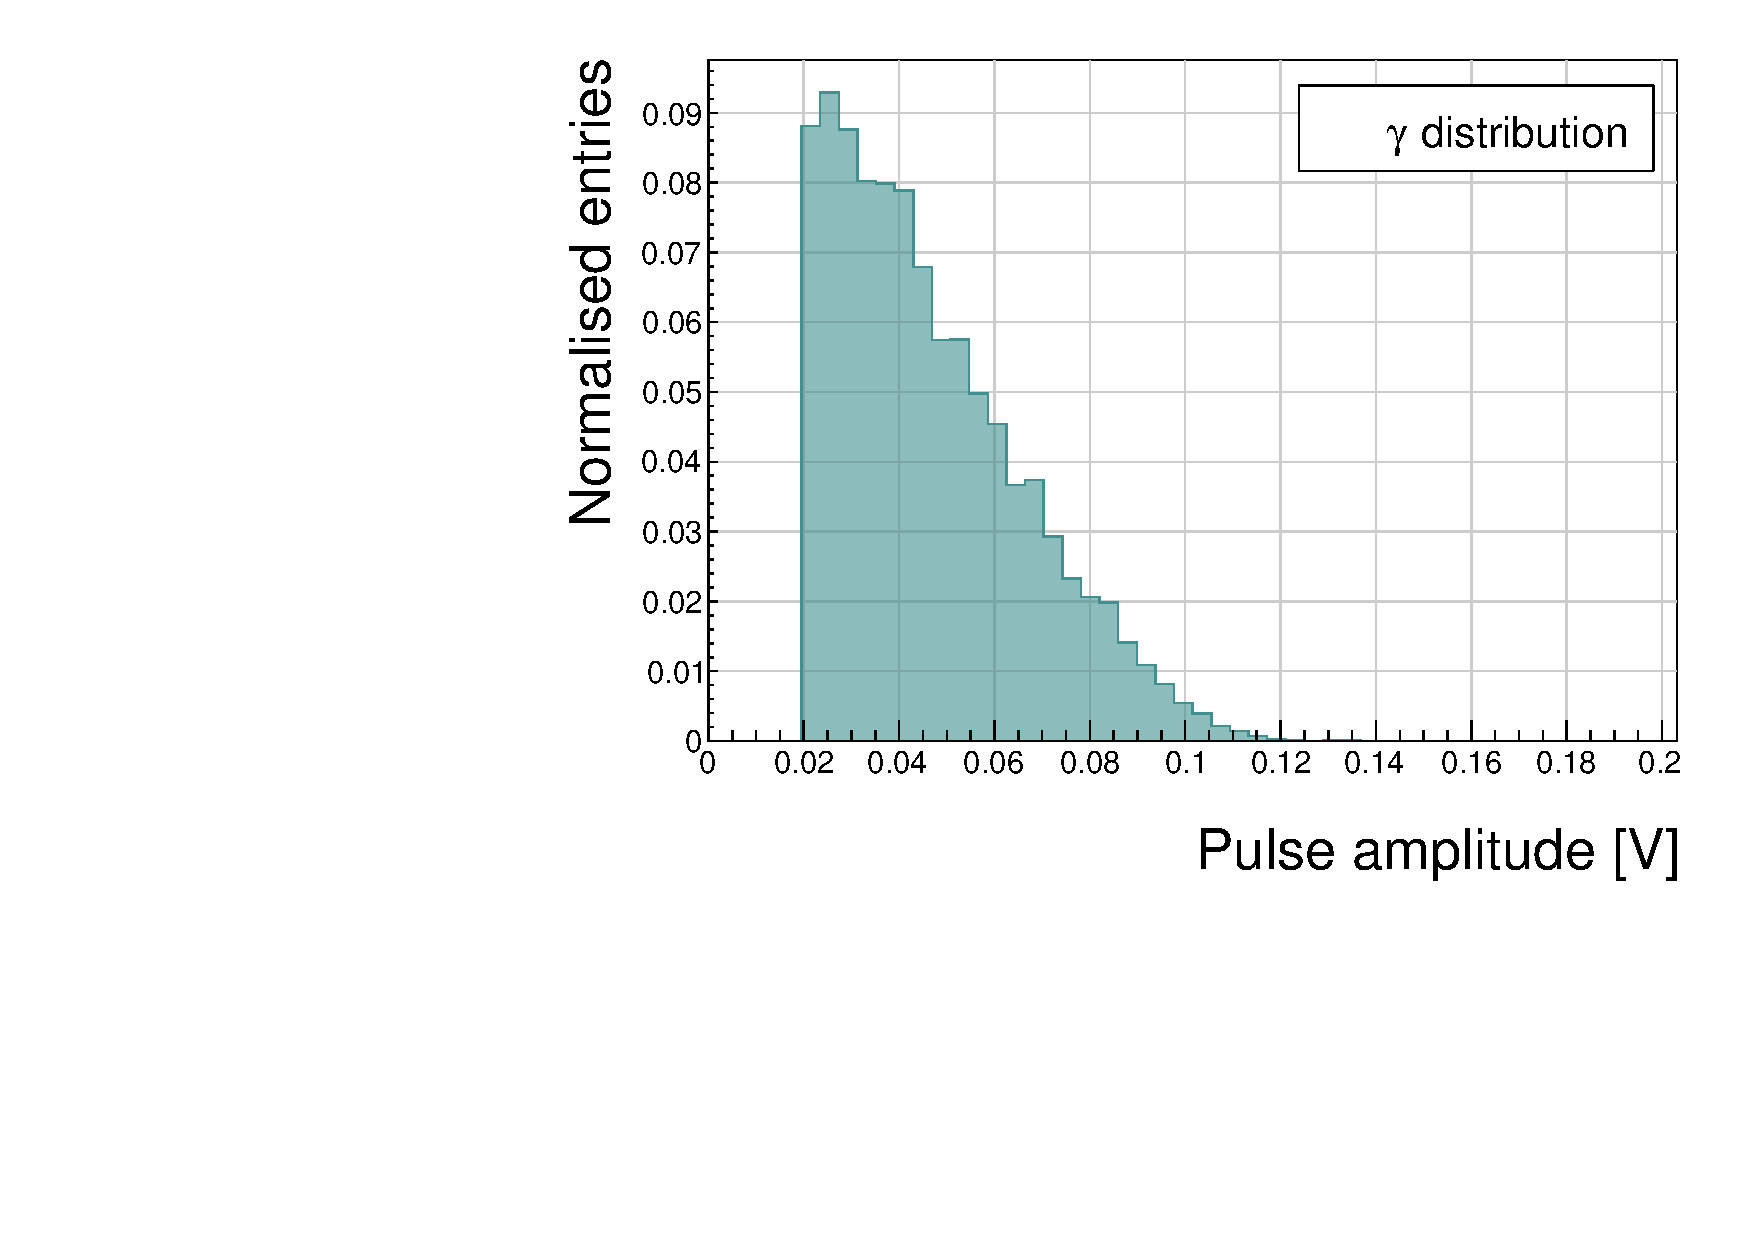
\includegraphics[width=0.47\textwidth]{03_measurement_results/scripts/plots/samplePulses/gammadist}  \label{fig:gammadist1}} 
\end{tabular}
\caption{Superimposed and averaged pulses (left figures, current amplifier) and distributions of deposited energy (right figures, charge amplifier) for three types of radiation. Note the scale on the x axis of the distributions.}
\label{fig:pulsesaby}
\end{figure}




% Taken out due to repetition. Maybe a small part will be moved to Ch 2.
%%---------------------------------------------------------------------------------------------------------------
%%%\clearpage
%\subsection{Noise limitations}
%\label{sec:noiselimit}
%%---------------------------------------------------------------------------------------------------------------
%%TO DO: Take 8 runs with the 2GHz oscilloscope while increasing the noise. 
%%TO DO: leakage current, irradiated.
%Noise is a major limiting factor in particle detection. It defines the minimum measurable particle energy and the minimum measurement resolution. It is hence important to minimise the electric noise in the detector signal. The major noise contribution comes from poor shielding from external electromagnetic sources. These often cause ringing whereby the signal oscillates with a frequency defined by the external source. The ringing makes high-frequency measurements impossible. Another source of noise is the sensor itself. In the case of silicon, natural light increases the number of thermally excited free charge carriers, increasing the leakage current. This is not the case for diamond, which is with its high energy band gap insensitive to visible light. Nevertheless, any noise produced by the sensors is amplified by the signal amplifiers, which add an additional noise of the analogue electrical circuit to the amplified signal. Finally, the digitisers add the quantisation noise to the digitised signal. If the measurement range is significantly higher than the actual measured signal, the quantisation noise can be a significant contributor to the decrease of the overall measurement resolution.






% ---------------------------------------------------------------------------------------------------------------
\clearpage
\section{Radiation limitations}
\label{sec:radlimit}
% ---------------------------------------------------------------------------------------------------------------
%3par merged in ch2
This section quantifies the decrease in charge collection efficiency as well as the effects on long-term measurement stability in irradiated sCVD diamonds.


\subsection{Irradiation study}
This subsection contains a study of the effects of 300~MeV pion irradiation on the charge collection efficiency of sCVD diamond detectors. To carry out this study, two diamond samples were irradiated with 300~MeV pions ($\uppi$, kinetic energy 191.31~MeV). The irradiation campaign took place at the Paul Scherrer Institute (PSI)~\cite{PSI:00000} where the machine provides a flux of $1.5\times10^{14}~\pi$~cm$^{-2}$ per day. The quoted uncertainty on the measurement of the delivered dose is $\pm20~\%$. In addition, a deviation in beam energy can have a significant effect on the damage in the sensor, considering the pion damage curve in figure~\ref{fig:kitdpa} at a $\pi_{\mathrm{300~MeV}}$ point (~191~MeV kinetic energy), which sits on a steep section of the DPA curve. The target fluences for S79 and S52 were  (1$\pm0.2$)$\times10^{14}~\pi$~cm$^{-2}$ and (3.6$\pm0.7$)$\times10^{14}~\pi$~cm$^{-2}$.

A test beam campaign was carried out to observe the charge collection efficiency at different bias voltage settings. The efficiency values acquired are used to determine the effective drop in efficiency as a function of fluence. This is to test if the collected charge $Q$ is inversely proportional to the fluence $\Phi$, as per equation~\ref{eq:radfactor1}. A procedure defined by a collaboration researching diamond behaviour RD42 has been applied to the measured values to extract the damage factor described in section~\ref{sec:raddam}.

Subsection~\ref{sec:longterm} contains measurements and results of a long-term stability study using $\upalpha$ and $\upbeta$ particles. In particular, charge collection efficiency with $\upbeta$ and $\upalpha$ radiation as a function of time is measured. To investigate the effect of decreased charge collection of irradiated diamond with time, TCT (transient current technique) is employed. Finally, a procedure that improves the pulse shapes and the charge collection efficiency is proposed.



%\subsubsection{Irradiation with a 300~MeV $\uppi$  beam}

%After fitting a linear function between, the error on the DPA due to the uncertainty on the beam energy amounts to 7~\%. Overall error on the fluency is therefore the root mean square of the uncertainty on the DPA and the uncertainty on the hardness factor: $\upsigma=21~\%$.

%Two diamond samples, S52 and S79, were put in the $\uppi_\mathrm{300~MeV}$ beam in the 2014 PSI irradiation campaign; S52 to $(1\pm0.2)\times10^{14}~\pi$~cm$^{-2}$ and S79 to $(3.6\pm0.7)\times10^{14}~\pi$~cm$^{-2}$. During the process, the gold electrodes got slightly activated, but the activation decayed in two weeks.

\subsubsection{300~MeV $\uppi$ radiation damage factor}
Three diamonds -- non-irradiated S37 and irradiated S52 and S79 -- were tested in a $\uppi_\mathrm{120~GeV/c}$ test beam in the SPS North Experimental Area at CERN~\cite{Brianti:604383} before and after irradiation. The goal was to estimate the charge collection efficiency and charge collection distance as a function of fluence. The samples were primed prior to data taking using a $^{90}$Sr radioactive source. The data were then taken at a range of bias voltages ranging from 30~V to 900~V, yielding between 0.06~V/$\upmu$m and 1.8~V/$\upmu$m electrical field in the bulk. Every data point contained approximately $5\times10^4$ measured particles. The charge deposited by the particles was measured using a CIVIDEC Cx charge preamplifier. 
%, as seen in figure~\ref{fig:landausample}. 

The integrated amplitude spectrum is a Landau distribution. Its most probable value (MPV) is used to calculate the most probable collected charge $Q_\mathrm{i}$:
\begin{equation}
\label{eq:ccdcalc}
Q_\mathrm{i}~[\mathrm{e}^-] 
= \frac{1} {1.6\times 10^{-19}} Q_\mathrm{i}~[\mathrm{C}] 
= 6'241 \cdot Q_\mathrm{i}~[\mathrm{fC}] 
= 6'241 \cdot \frac{MPV~[\mathrm{mV}]}{A~[\frac{\mathrm{mV}}{\mathrm{fC}}]}
,
\end{equation} 
where A$=9.3$~mV/fC is the preamplifier gain factor and 1~e$^-$~=~1.6$\times10^{-19}$~C. 

The CCD for the three measured samples at a bias voltages ranging from 0.2--1.6~V~$\upmu$m$^{-1}$ calculated using equation~\ref{eq:ccdcalc1} is shown in figure~\ref{fig:ccd}. S37 exhibits a full collection distance already at 0.4~V~$\upmu$m$^{-1}$ whereas the irradiated samples have a more gentle increase of CCD with increasing bias voltage. It is evident that at 1~V~$\upmu$m$^{-1}$  the maximum CCD has not been reached in the case of S79 and S52. Nevertheless, to compare the measured data point with those provided by RD42, the CCD at 1~V$\upmu$m$^{-1}$ has to be taken.

\begin{figure}[!t]
\begin{center}
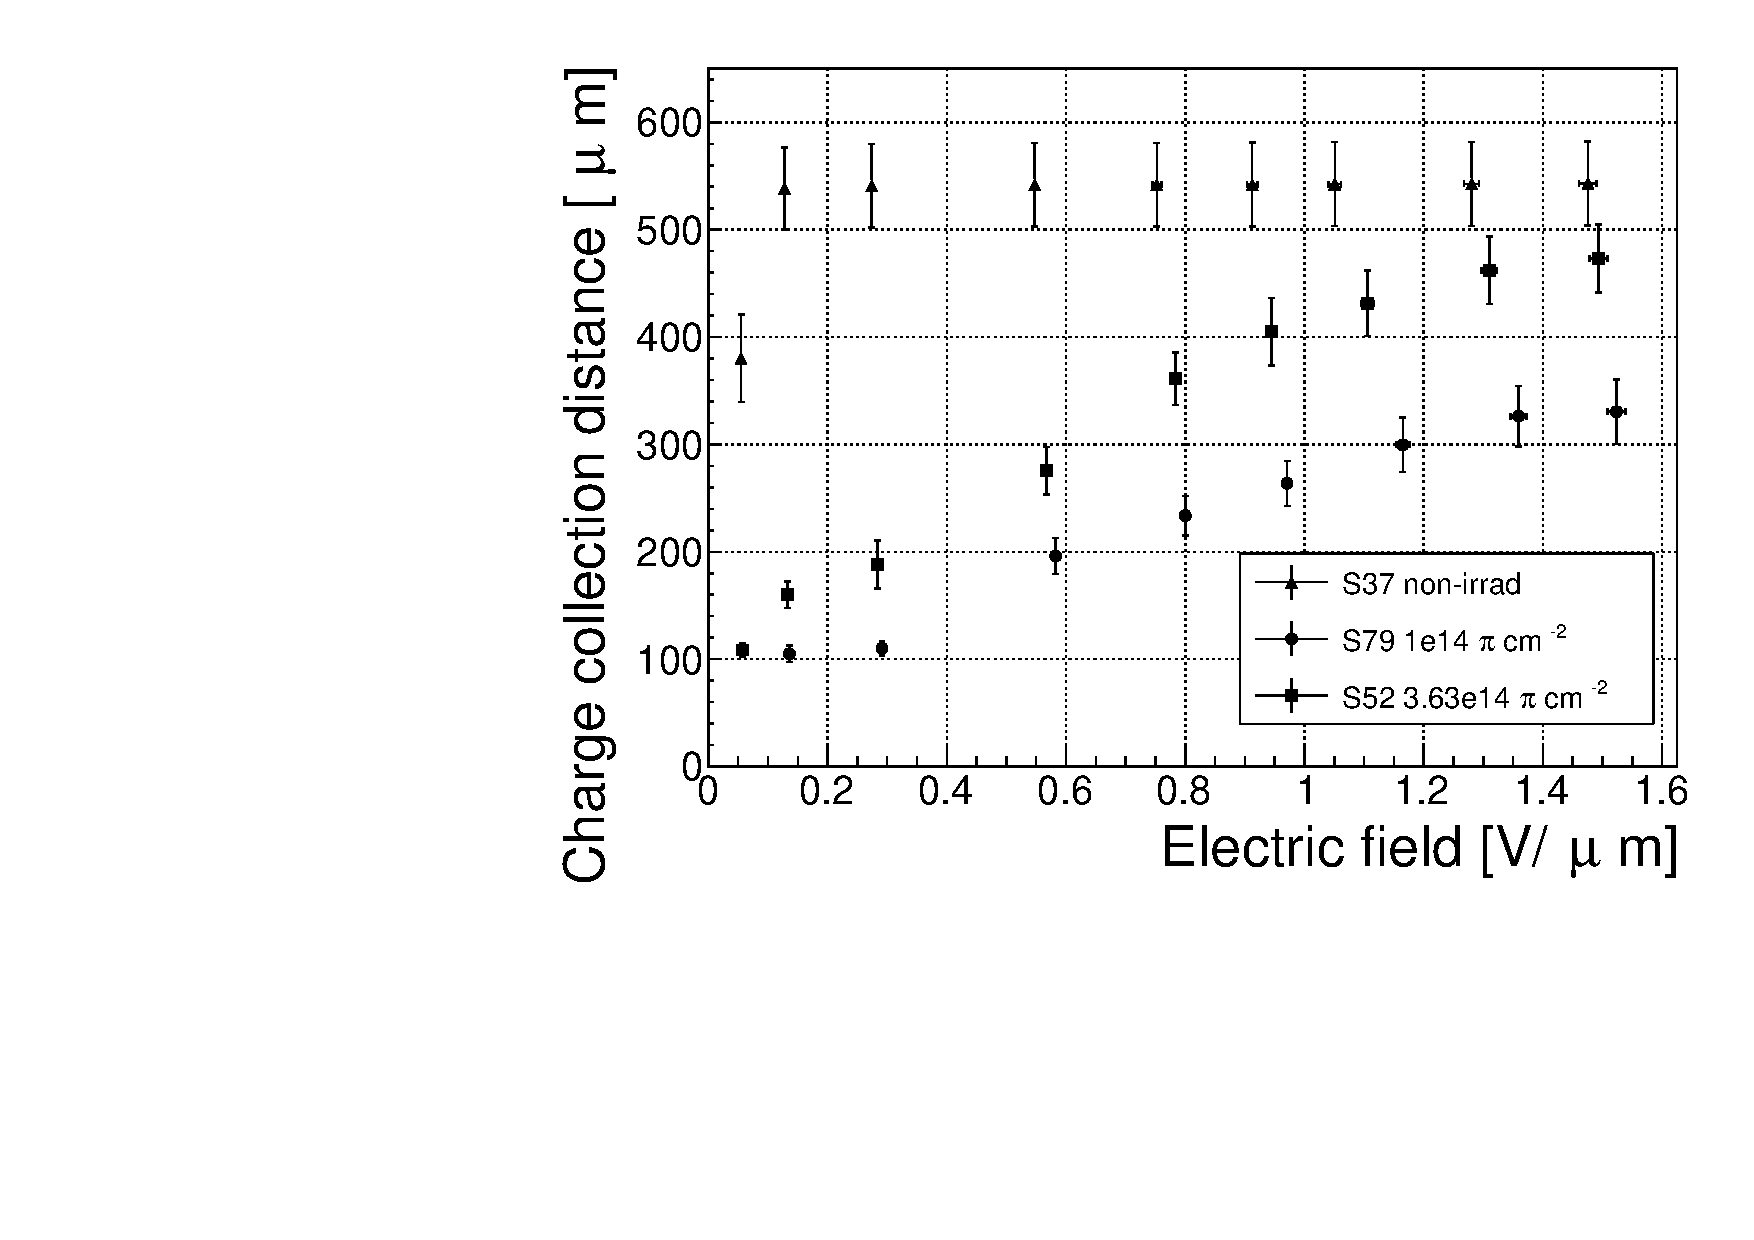
\includegraphics[width=0.7\textwidth]{03_measurement_results/scripts/plots/ccd}
\caption{The figure shows the CCD for S37, S79 and S52 at a range of bias voltage settings.}
\label{fig:ccd}
\end{center}
\end{figure}

Data points with the maximum CCD obtained in the test beam measurements are plotted as a function of fluence in figure~\ref{fig:radfactor}. Equation~\ref{eq:radfactor1} is fitted to the data points and a damage factor $k_{\mathrm{\lambda}}=(4.4\pm1.2)\times10^{-18}~\upmu$m$^{-1}$~cm$^{2}$ is obtained. The value is for a factor of two higher than the damage factor obtained by RD42. %The irradiated samples do not yet have a full charge collection at 1.0~V~$\upmu$m$^{-1}$. 
This could be due to an insufficient priming time ahead of the measurement. The samples were only exposed to the radioactive source for 30~min and might not have achieved the maximum charge collection (effect of priming shown in figure~\ref{fig:ccincrease}). In addition, the diamond samples have not been polished and re-metallised after irradiation, as is the case for the RD42. A study of effects of re-metallisation on the charge collection has been done in~\cite{pomorski2008electronic} and supports this theory. Furthermore, with only two samples measured, the statistical uncertainty is high. For a better fit another measurement point at a higher fluence would need to be added. Nevertheless, it can be concluded that the 300~MeV pions damage the diamond bulk significantly more than the 24~GeV protons, as shown in chapter~\ref{ch:diamond}.

Another diamond irradiation study has been carried out using the Beam Conditions Monitor (BCM) at the CMS experiment~\cite{Guthoff:1977429}. The BCM's diamond sensors have been exposed to radiation from beam collisions with a wide spectrum of energies and particle types. The damage factors measured are an average of $3.5\times10^{-17}~\upmu$m$^{-1}$~cm$^{2}$ and $9.2\times10^{-16}~\upmu$m$^{-1}$~cm$^{2}$ for pCVD and sCVD diamonds, which is for a factor of 58 and 1500 higher than the RD42. These low charge collection efficiencies, however, are purported to be convoluted with other effects, such as polarisation, which will be discussed later in the chapter.


\begin{figure}[!t]
\centering
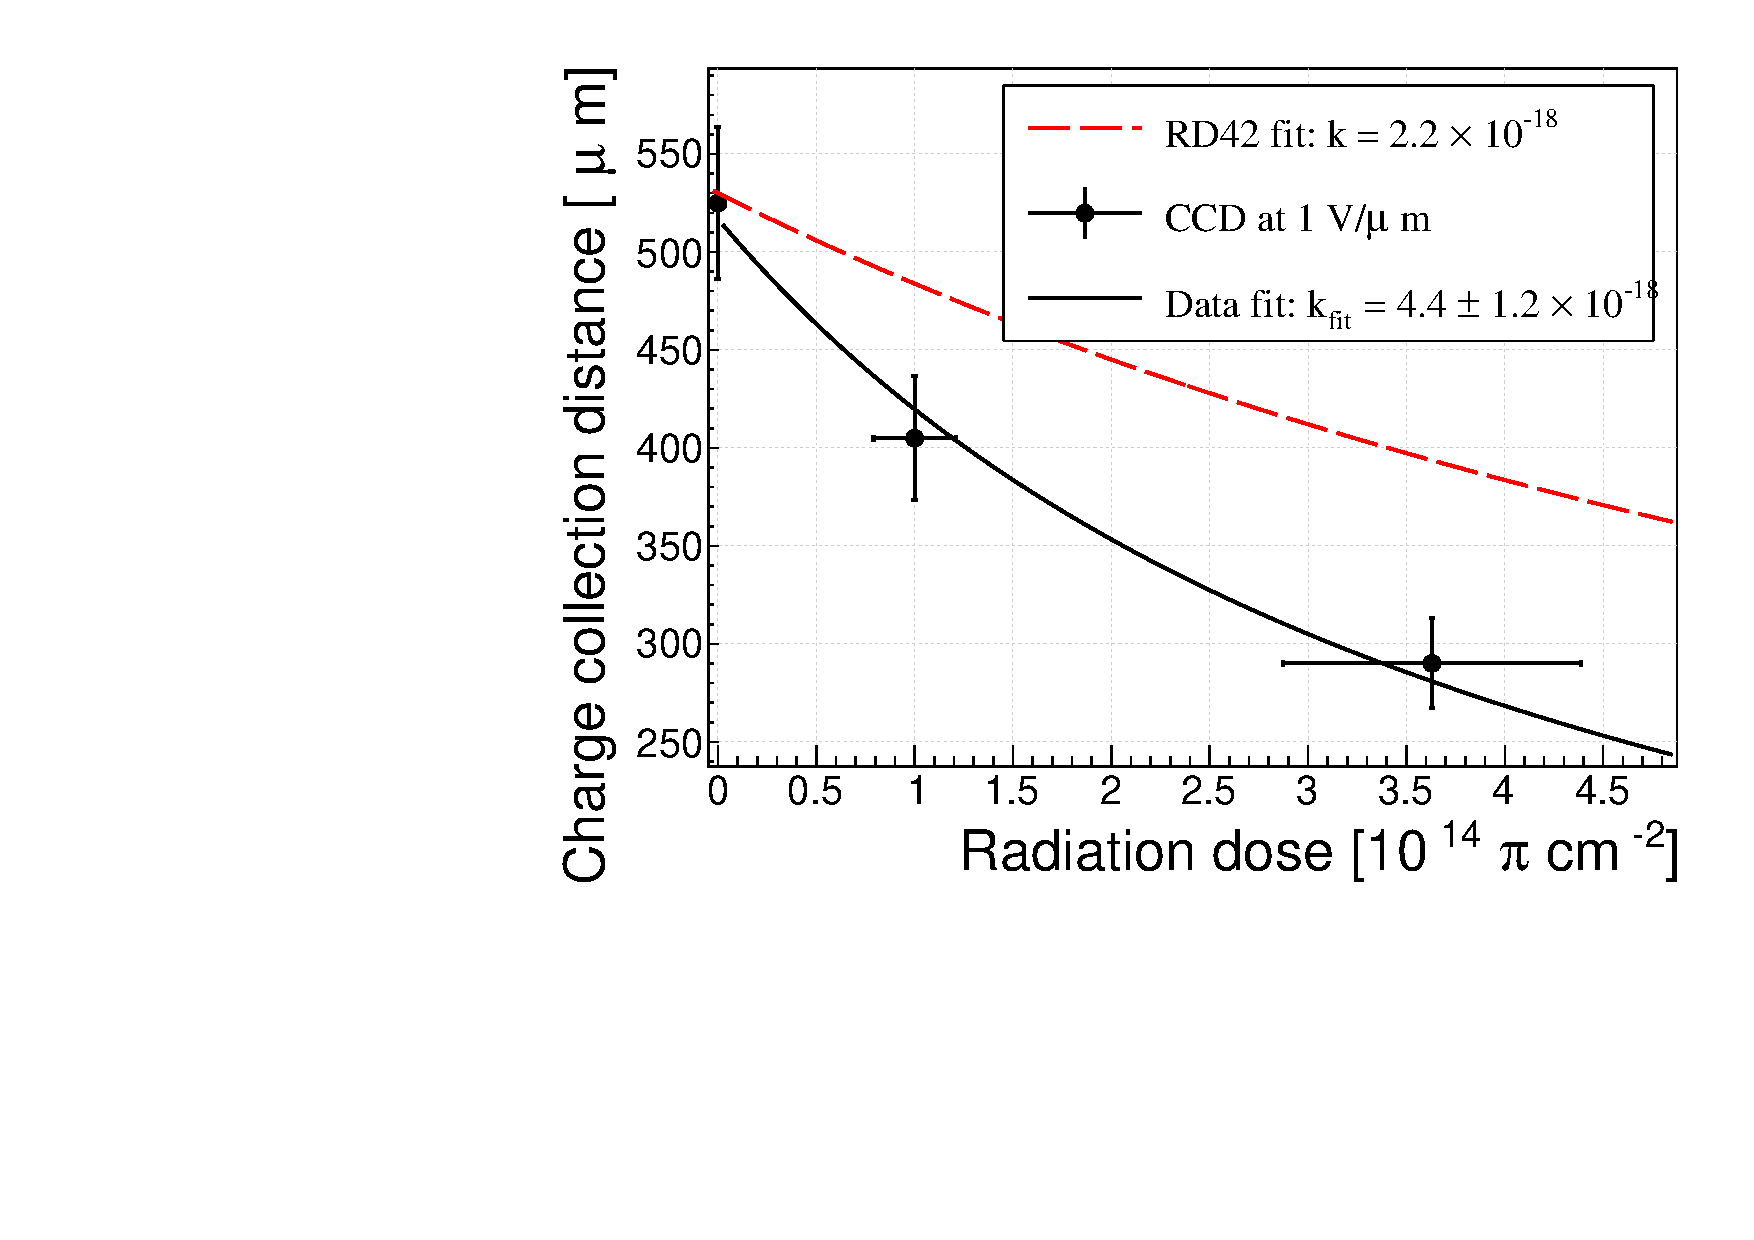
\includegraphics[width=0.70\textwidth]{03_measurement_results/scripts/plots/radfactor1}
\caption{The charge collection distance at 1~V/$\upmu$m bias voltage for the three diamond samples is plotted as a function of fluence. It is compared to the RD42 data for pion irradiation. The data points are about 15--25~\% lower than expected from the RD42 data~\cite{RD42IRRAD:00000}.}
 \label{fig:radfactor}
\end{figure}



%------------------------------------------------------------------------------------------------------------
\subsection{Long-term measurement stability}
\label{sec:longterm}
An important requirement for particle detectors is a stable performance over long periods of time. For instance, charge collection for a defined radiation type and quantity must not change over time or has to change in a predicted way. The stability of diamond detectors depends on many factors, e.g. material purity, polishing process, electrode material, irradiation damage etc. The aim is to study the behaviour of diamond under controlled conditions, with the goal to understand its limitations. One of these limitations is the fluence as it can affect the long-term stability of the sensor during operation. 

The three diamond samples (S37, S79 and S52) have been exposed to two different types of ionising radiation for a longer period to see if their behaviour changes over time. Two parameters have been observed in particular: 
\begin{enumerate}
\item Charge collection of $\upbeta$ particles and 
\item Charge collection and ionisation profile of $\upalpha$ particles.
\end{enumerate}
%NOTE I can use this part for conclusion. Don't write the ABSTRACT!
%The results in this and in the following section show that priming plays an important role in improving the diamond measurement stability in both cases. 
%The $\upbeta$ particles have a ``healing'' effect on the diamond; MIP detection is therefore rather stable in the long run, despite the fact that the sensors had been degraded by means of irradiation. Alpha particles, on the other hand, deteriorate the measurement, probably by introducing space charge into the sensor bulk. 

%----------------------------------------------------------------------------------------------------------------------
\subsubsection{$\upbeta$ long-term stability}
The diamond samples have undergone a long-term stability test at room temperature using $\upbeta$ radiation. This has been done using a $^{90}$Sr source emitting $\sim$2.28~MeV electrons via $^{90}$Y decay at a rate of approximately $10^4$~e$^-$~cm$^{-2}$~s$^{-1}$ as measured using a real-time particle counting application described in chapter~\ref{ch:cur}. To simulate the initial conditions in HEP experiments, the sensors must not be primed before starting the measurements. The measurement setup consists of a diamond sample (S37, S52 or S79) with the CIVIDEC Cx spectroscopic amplifier, a silicon diode with a CIVIDEC C6 amplifier for triggering and a $^{90}$Sr source on top. A particle emitted by the source traverses the sensor bulk and hits the silicon diode, triggering the analogue signal readout. The source is left on the top for the course of the experiment. The measurements, however, are taken at discrete times. For every data point, approximately $10^4$ triggers have to be recorded. The offline analysis of the recorded signal pulse amplitudes yields a Landau distribution for every data point. The current charge collection relative to the initial charge collection for every sample is plotted as a function of the received $\upbeta$ dose in figure~\ref{fig:ccincrease}. It shows that, for the irradiated samples, the charge collection efficiency improves when the diamond sensor is primed with a $\upbeta$ source. The effect is negligible for the non-irradiated high-quality S37. Both relative increases are significant -- 22~\% for S79 and 55~\% for S52. At a fluence of approximately 4$\times10^6$~particles the charge collection is stabilised. At that point S79 achieves close to a full efficiency (in absolute values -- not shown) whereas S52 reaches approximately 50~\%.

%The $\sim$2.28~MeV electrons emitted by this source are not MIPs; their charge deposition is higher than that of an electron MIP, according to the Bethe-Bloch distribution~\cite{BETHE:00000}. Nevertheless, for the purpose of these measurements this energy is adequate since only the relative change in charge collection is of interest.

To sum up, diamond provides a stable measurement of the $\upbeta$ radiation detection after reaching a stable state. Even if damaged by radiation, it reaches a stable charge collection at a fluence of $\sim$4$\times10^6$~MIPs. Its efficiency decreases with a high fluence. %(effects visible above 10$^{12}$~MIP~cm$^{-2}$). 
However, the decrease can be accounted for if the damage factor and the rate and energy of the particles are known. $\upgamma$ radiation has a similar impact on the diamond as the $\upbeta$. The incident photons, if they interact with the diamond, prime the bulk, increasing the charge collection efficiency. The difference, however, is that the interaction probability (cross-section) is lower for gammas~\cite{sarin2014comprehensive,Griesmayer20121997}.

%%longterm pumping plot
\begin{figure}[!t]
\begin{center}
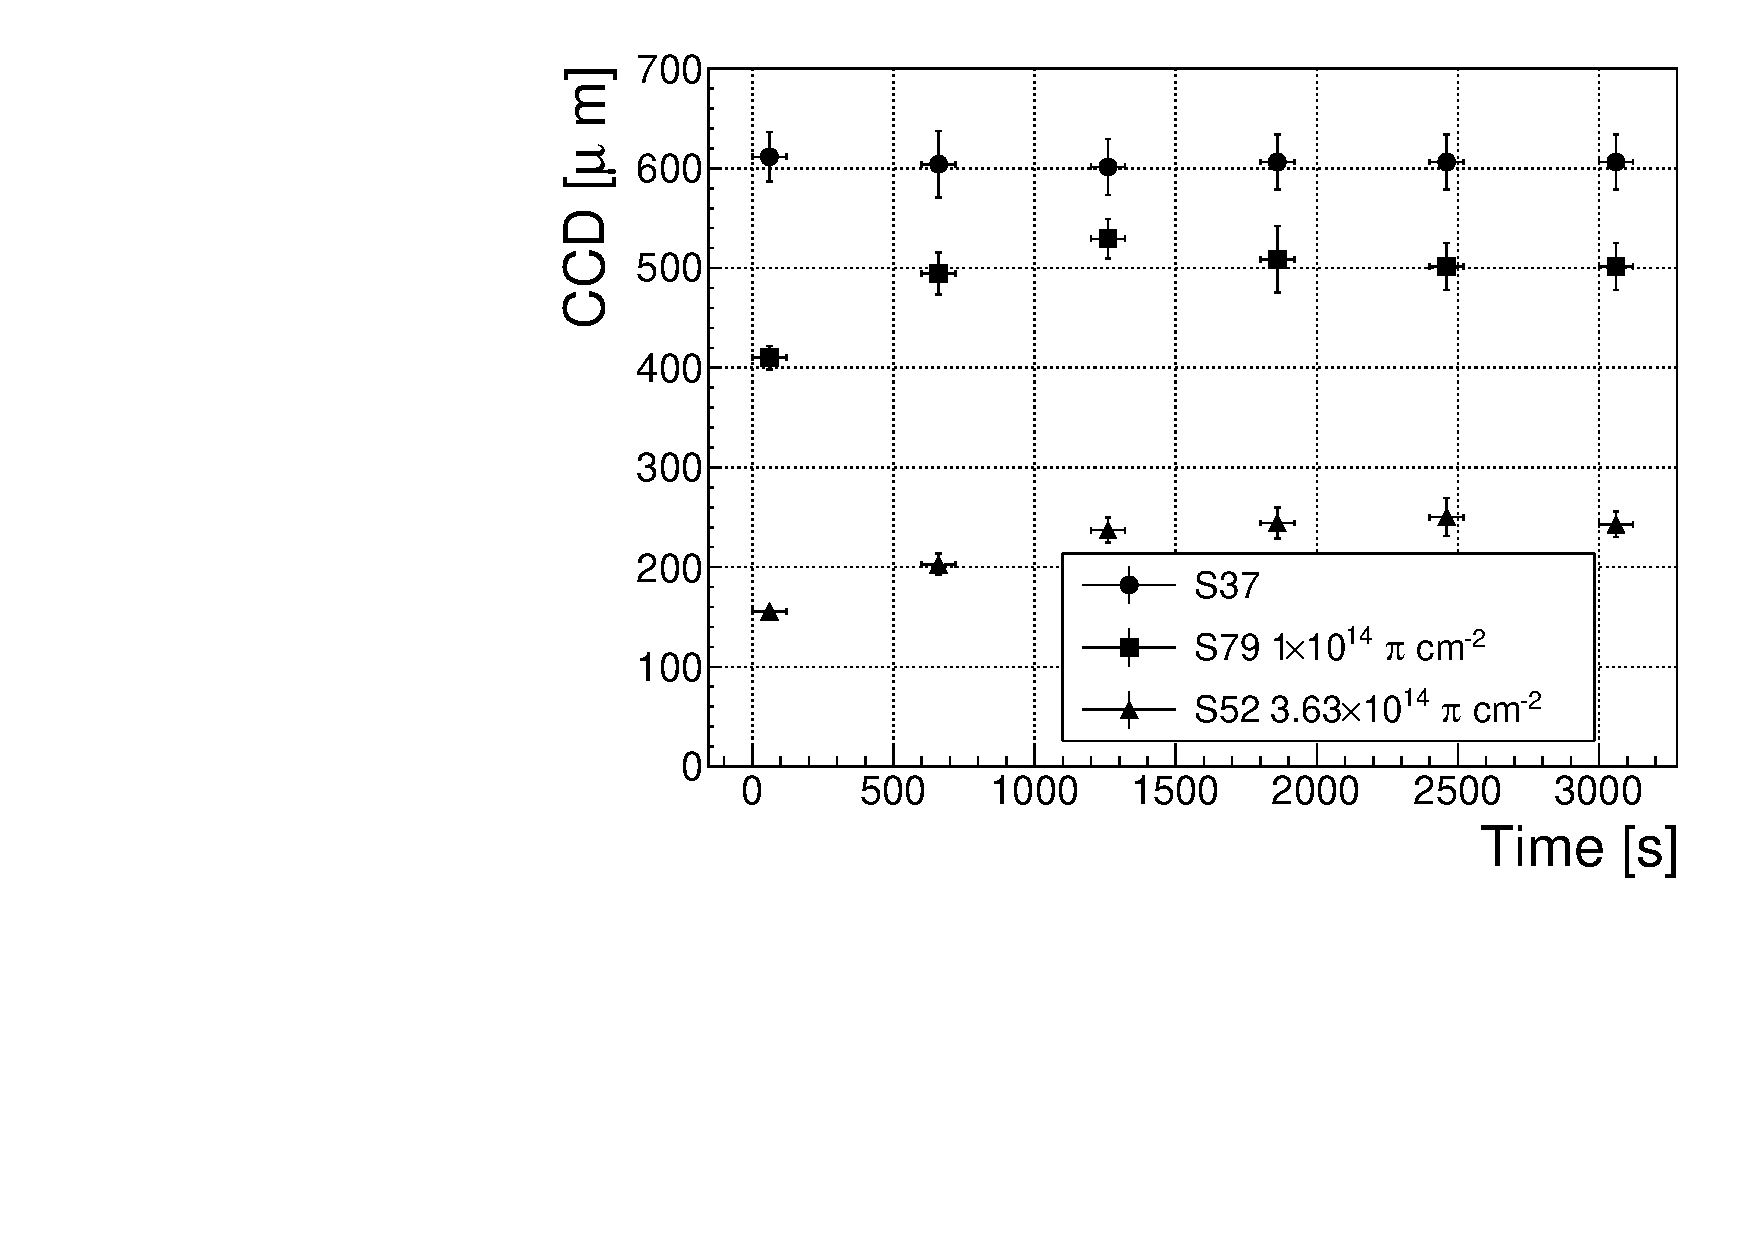
\includegraphics[width=0.7\textwidth]{03_measurement_results/plots/ccdpriming}
\caption{Relative increase of charge collection over time due to priming with the $^{90}$Sr radioactive source. The charge collection for the non-irradiated S37 stays constant. The bias voltage for this measurement is 1~V/$\upmu$m.}
\label{fig:ccincrease}
\end{center}
\end{figure}

%------------------------------------------------------------------------------------------------------------------------
\subsubsection{$\upalpha$ long-term stability}
This part discusses the stability of irradiated diamond sensors during $\upalpha$ measurements. An $^{241}$Am source has been used, emitting $\upalpha$ particles with a mean energy of 5.5~MeV with an average rate of 7~s$^{-1}$. 

%The measurement setup consisted of a PCB carrier for a diamond with a fitted $^{241}$Am source and a vacuum chamber. The carrier was placed into the chamber, which was then evacuated. t acted as shielding for external noise pickup and ensured that the $\upalpha$ particles didn't lose energy traveling through air. An SMA feedthrough ensured the electrical connection to the outside. The samples were measured before and after priming, at both polarities, to compare the behaviour of both electrons and holes as charge carriers. The scope of the measurements was to observe the changes in charge collection efficiency and/or in the pulse shapes. 

To test the stability of the diamond during $\upalpha$ measurements, the samples have been biased at +500~V and exposed to up to $8\times10^3$~$\upalpha$ hits while measuring their charge collection efficiency using the CIVIDEC Cx spectroscopic amplifier. The charge collected at every measurement point $Q(\Phi)$ is compared to collected charge of the first measurement $Q(0)$. The resulting ratio $\frac{Q(\Phi)}{Q(0)}$ for all samples is shown in figure~\ref{fig:longtermcx}. Each measurement point is an average of 30 consecutive $\upalpha$ hits. The observations are the following:
\begin{itemize}
\item[-] $Q(\Phi)$ for the non-irradiated S37 is stable as compared to $Q(0)$ over the course of the measurement.
\item[-] The initial efficiency of the irradiated S52 and S79 starts decreasing already at a low $\upalpha$ count.
\item[-] The charge collection efficiency of the unprimed irradiated samples drops much faster than after priming.
\item[-] The particle count rate decreases with decreased efficiency, which is clearly seen in the unprimed S52 data where the data points at a low efficiency are much further apart.
\end{itemize}
The absolute values are not shown here because only the relative drop is of interest in the scope of the long-term stability tests.

\begin{figure}[!t]
\begin{center}
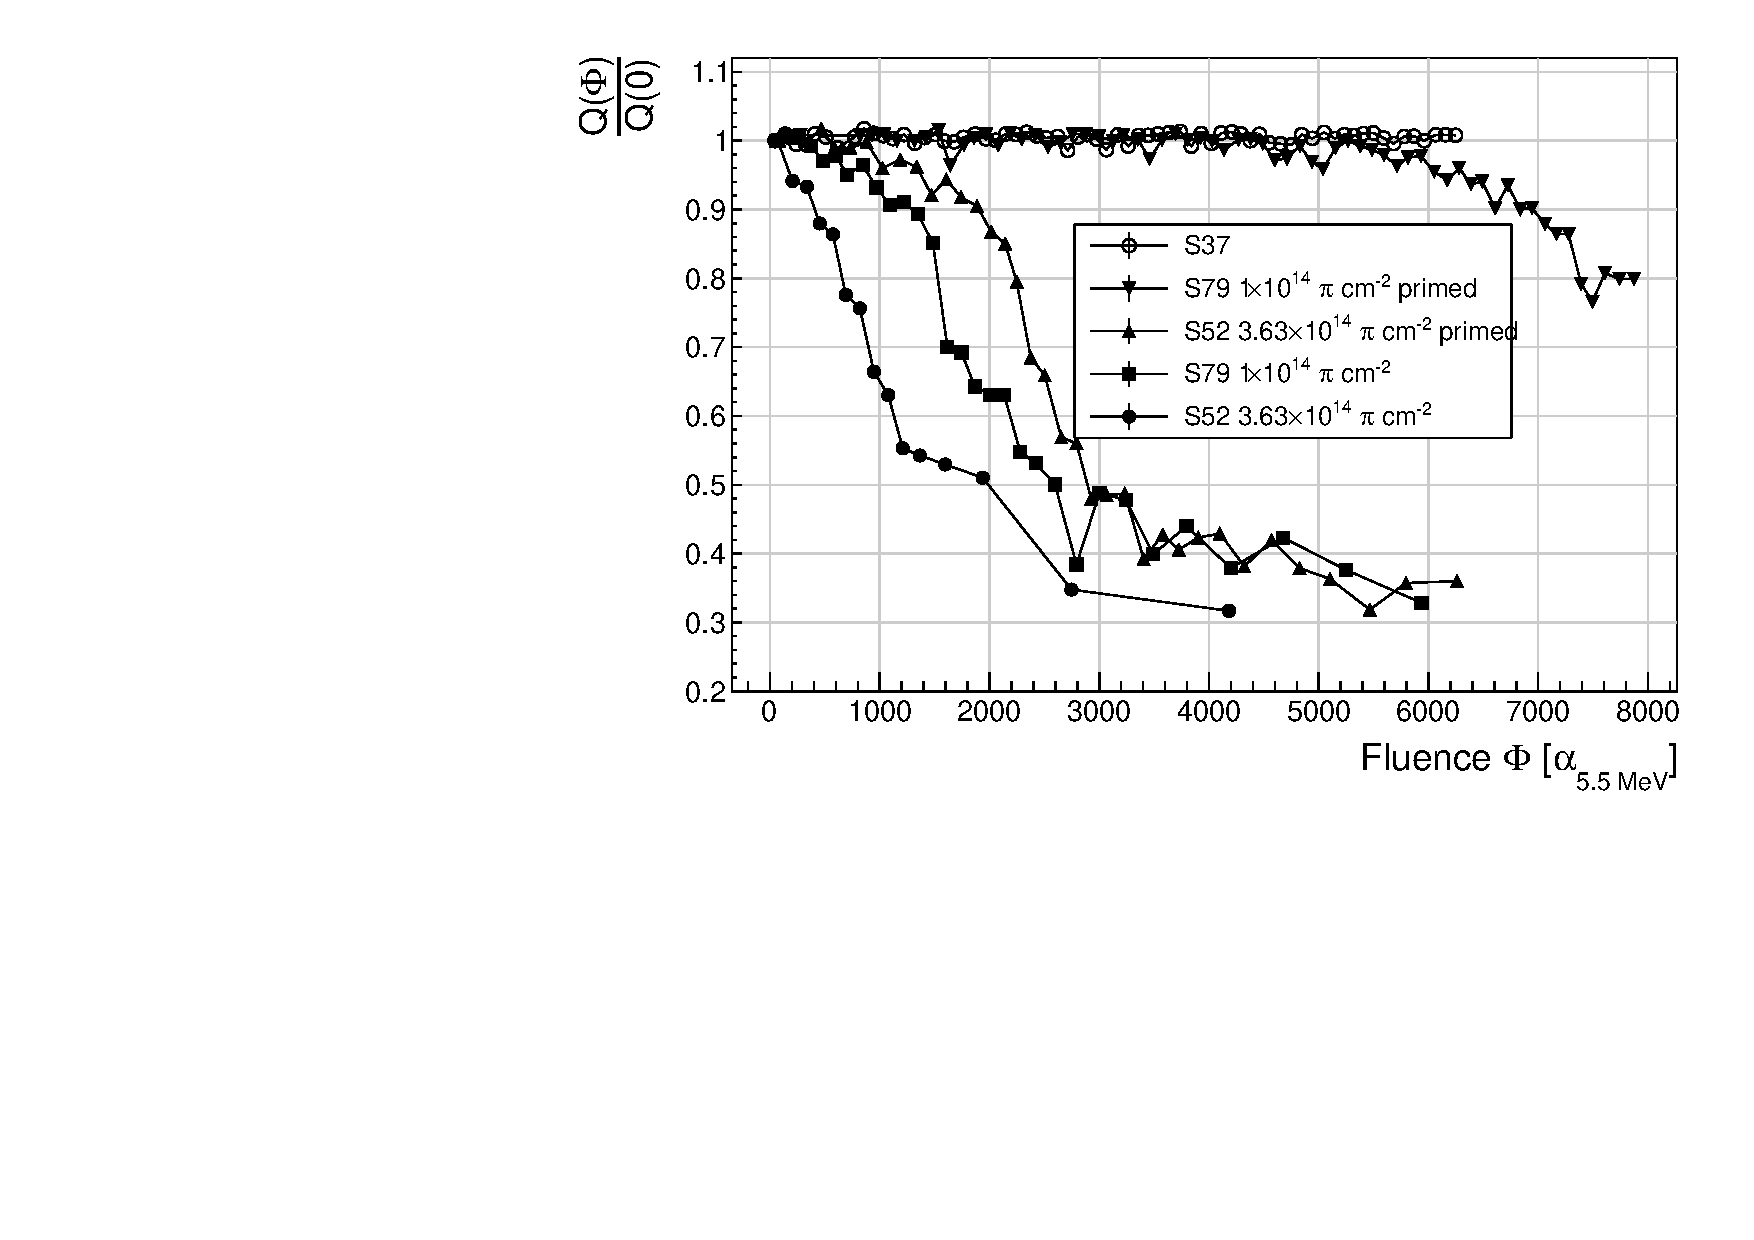
\includegraphics[width=0.7\textwidth]{03_measurement_results/scripts/plots/amplvstimecx4}
\caption{A relative drop in charge collection efficiency as a function of the received $\upalpha$ dose for non-irradiated and irradiated diamond samples.}
\label{fig:longtermcx}
\end{center}
\end{figure}

%the diamond bulk has been damaged by irradiation, these phenomena combined might have an effect on the operation of the detector.
%Figure~\ref{fig:longtermcx} shows the results of 6500 recorded hits at a rate of $\sim$7~particles per second.
%It is expected that the irradiated samples have a lower charge collection efficiency than the non-irradiated sample. 
%drops after a certain period of time. 
%The initial efficiency after priming with $\upbeta$ particles is higher than that without priming, but eventually it also deteriorates. In addition, the spread of measured energies increases significantly. This can not be seen in the figure as only the mean value of the data points is shown. Finally, the particle counting rate decreases with a decreased efficiency, which can be seen in the figure as the measurement points being further apart with the increasing dose (most pronounced for the un-primed S52). 


To investigate this sudden drop in efficiency, the current pulse shapes using a CIVIDEC C2 current amplifier have to be observed, as shown in figure~\ref{fig:lifetimeelecsholes}. The shape of the pulse holds more information about the charge carrier properties in the sensor than solely the value of the integrated charge. This time only the primed S79 sample has been tested. Both the hole and the electron collection are observed to determine whether they behave differently or not. 

The first observation in the raw acquired data in figures~\ref{fig:lifetimeelecsholes} is that the initially stable pulses start deteriorating; several different shapes start appearing gradually, some still very similar to those from the beginning while the others with almost zero amplitude. 

\begin{figure}[!t]
\centering
\begin{tabular}{rrr}
\subfloat{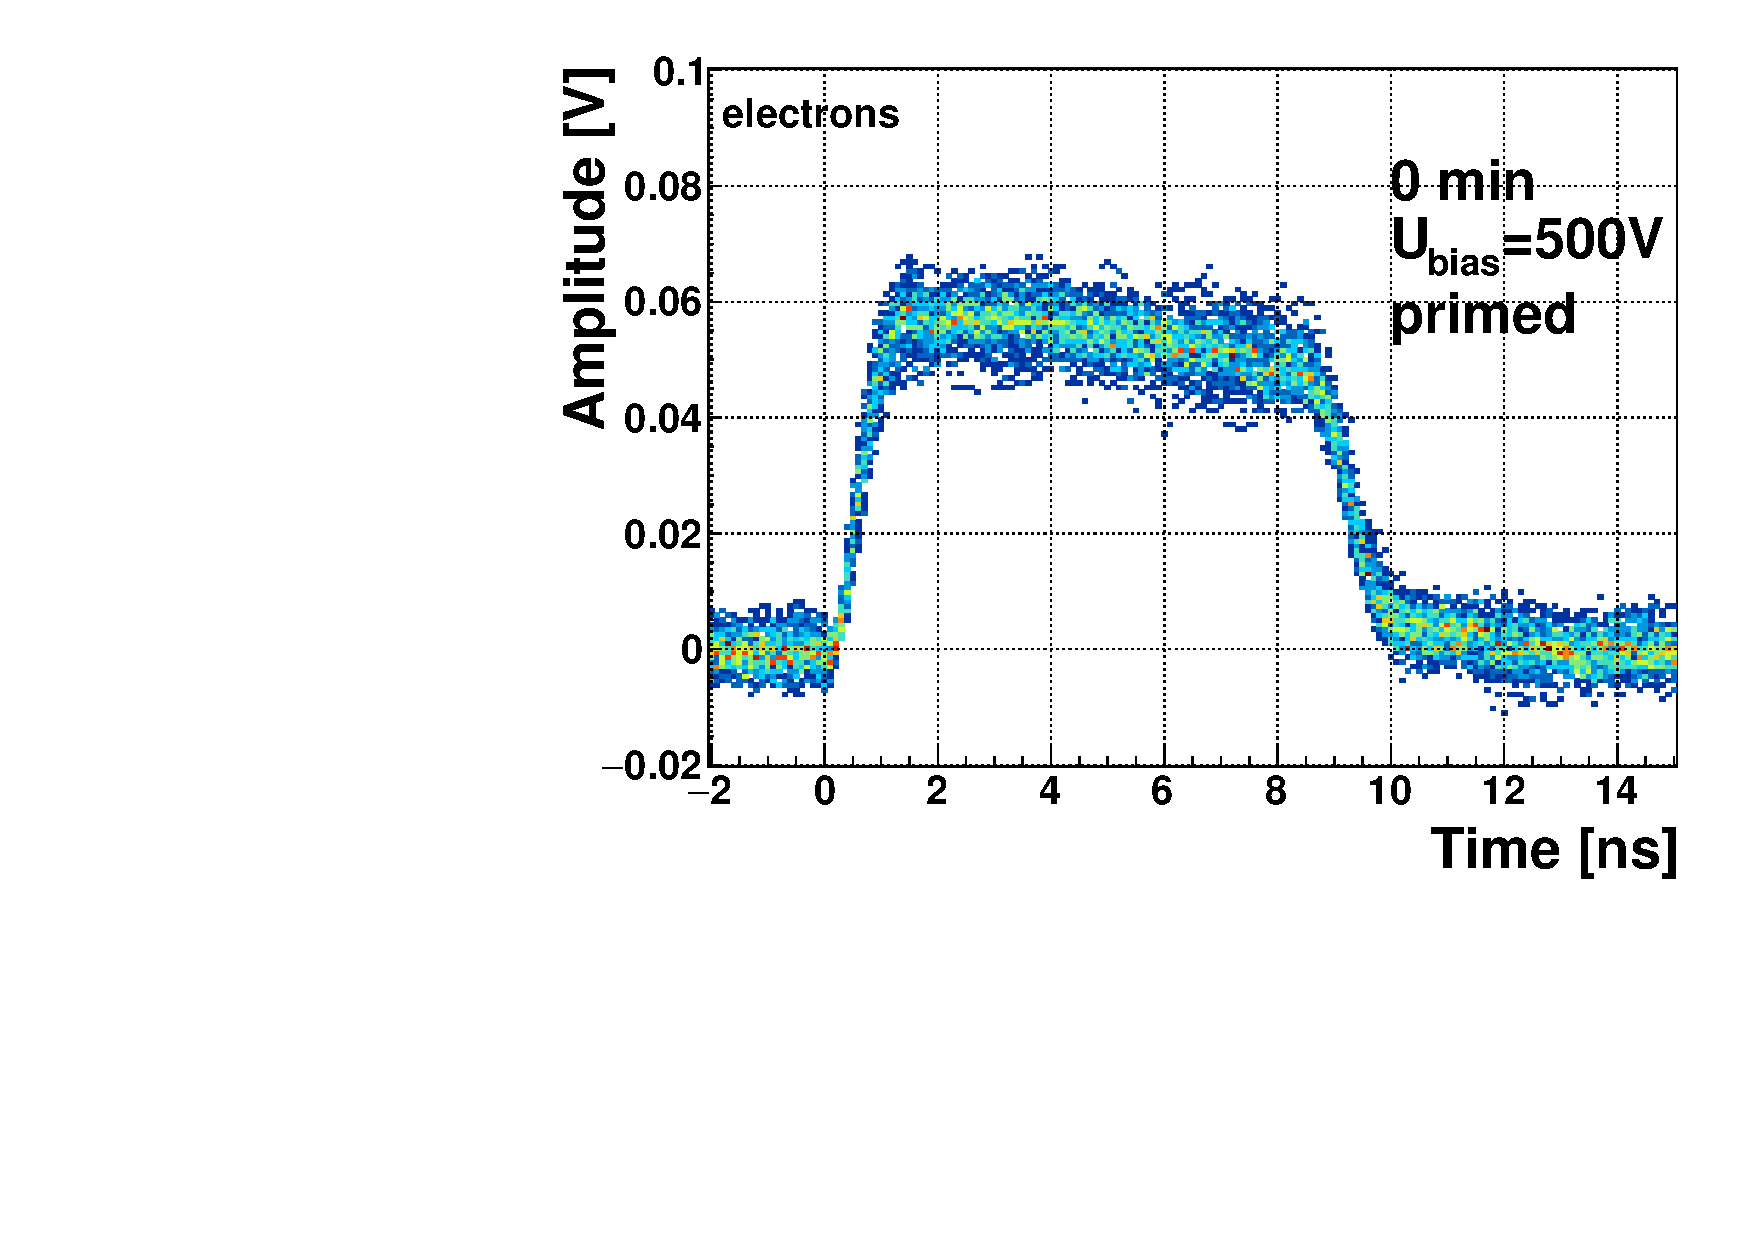
\includegraphics[width=0.47\textwidth]{03_measurement_results/scripts/plots/plotLifetime/elecs0} \label{fig:elecs0lt}} &
\subfloat{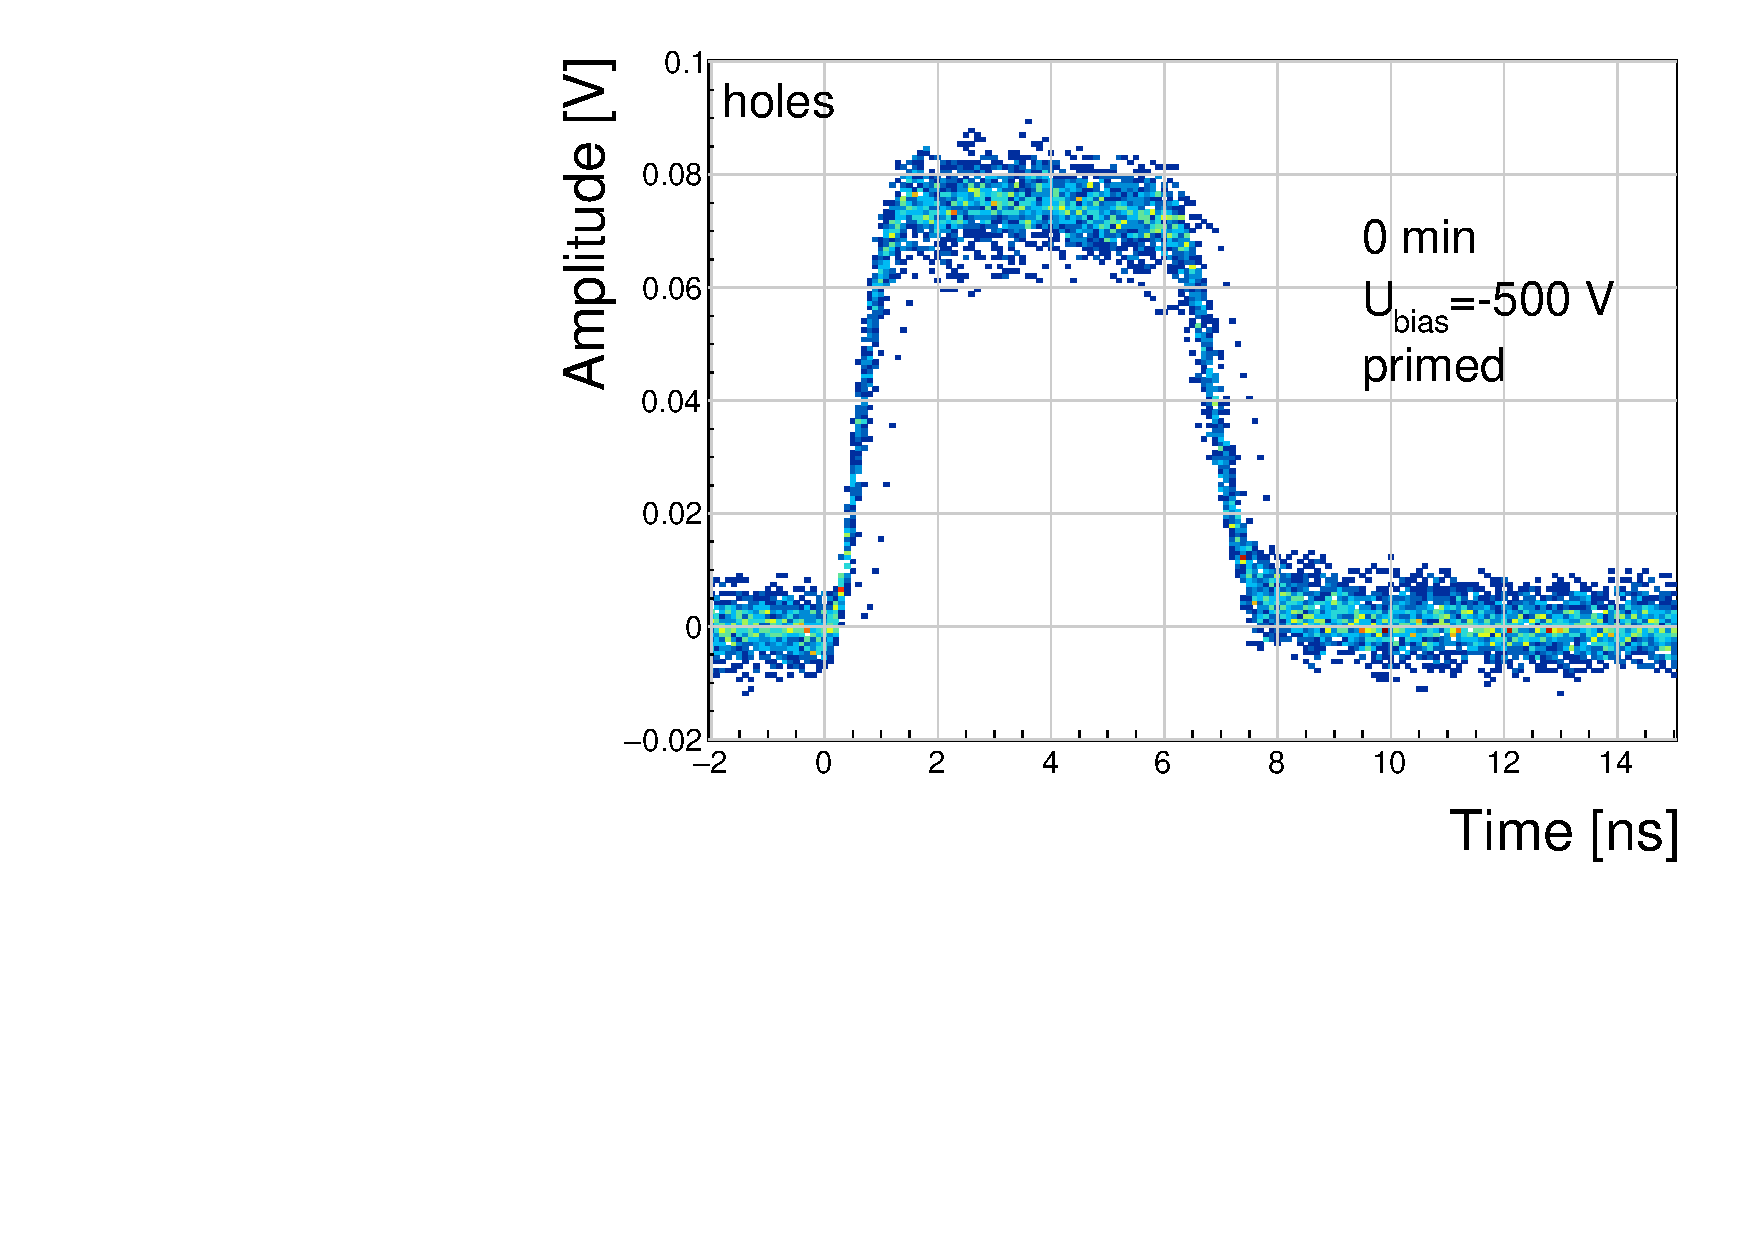
\includegraphics[width=0.47\textwidth]{03_measurement_results/scripts/plots/plotLifetime/holes0} \label{fig:holes0lt}} \\
\subfloat{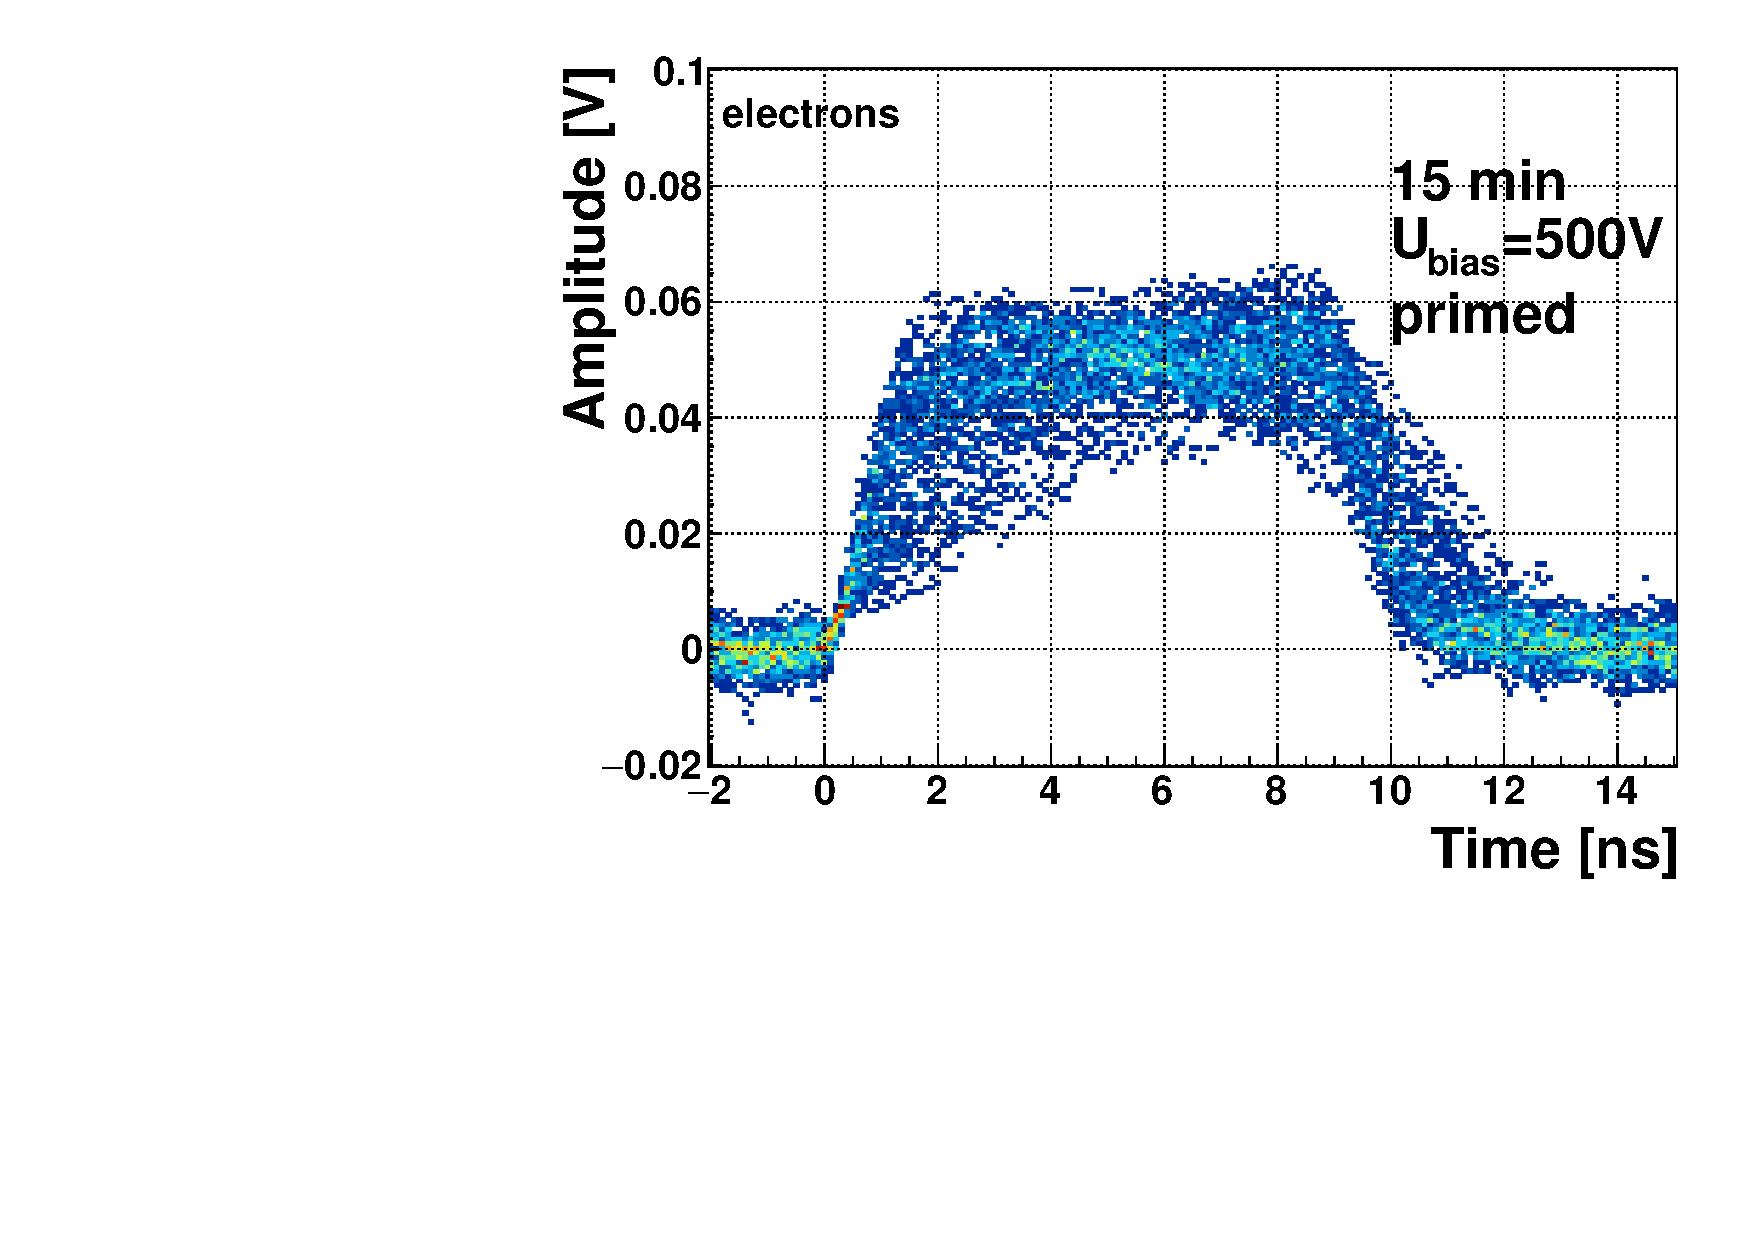
\includegraphics[width=0.47\textwidth]{03_measurement_results/scripts/plots/plotLifetime/elecs15}  \label{fig:elecs15lt}} &
\subfloat{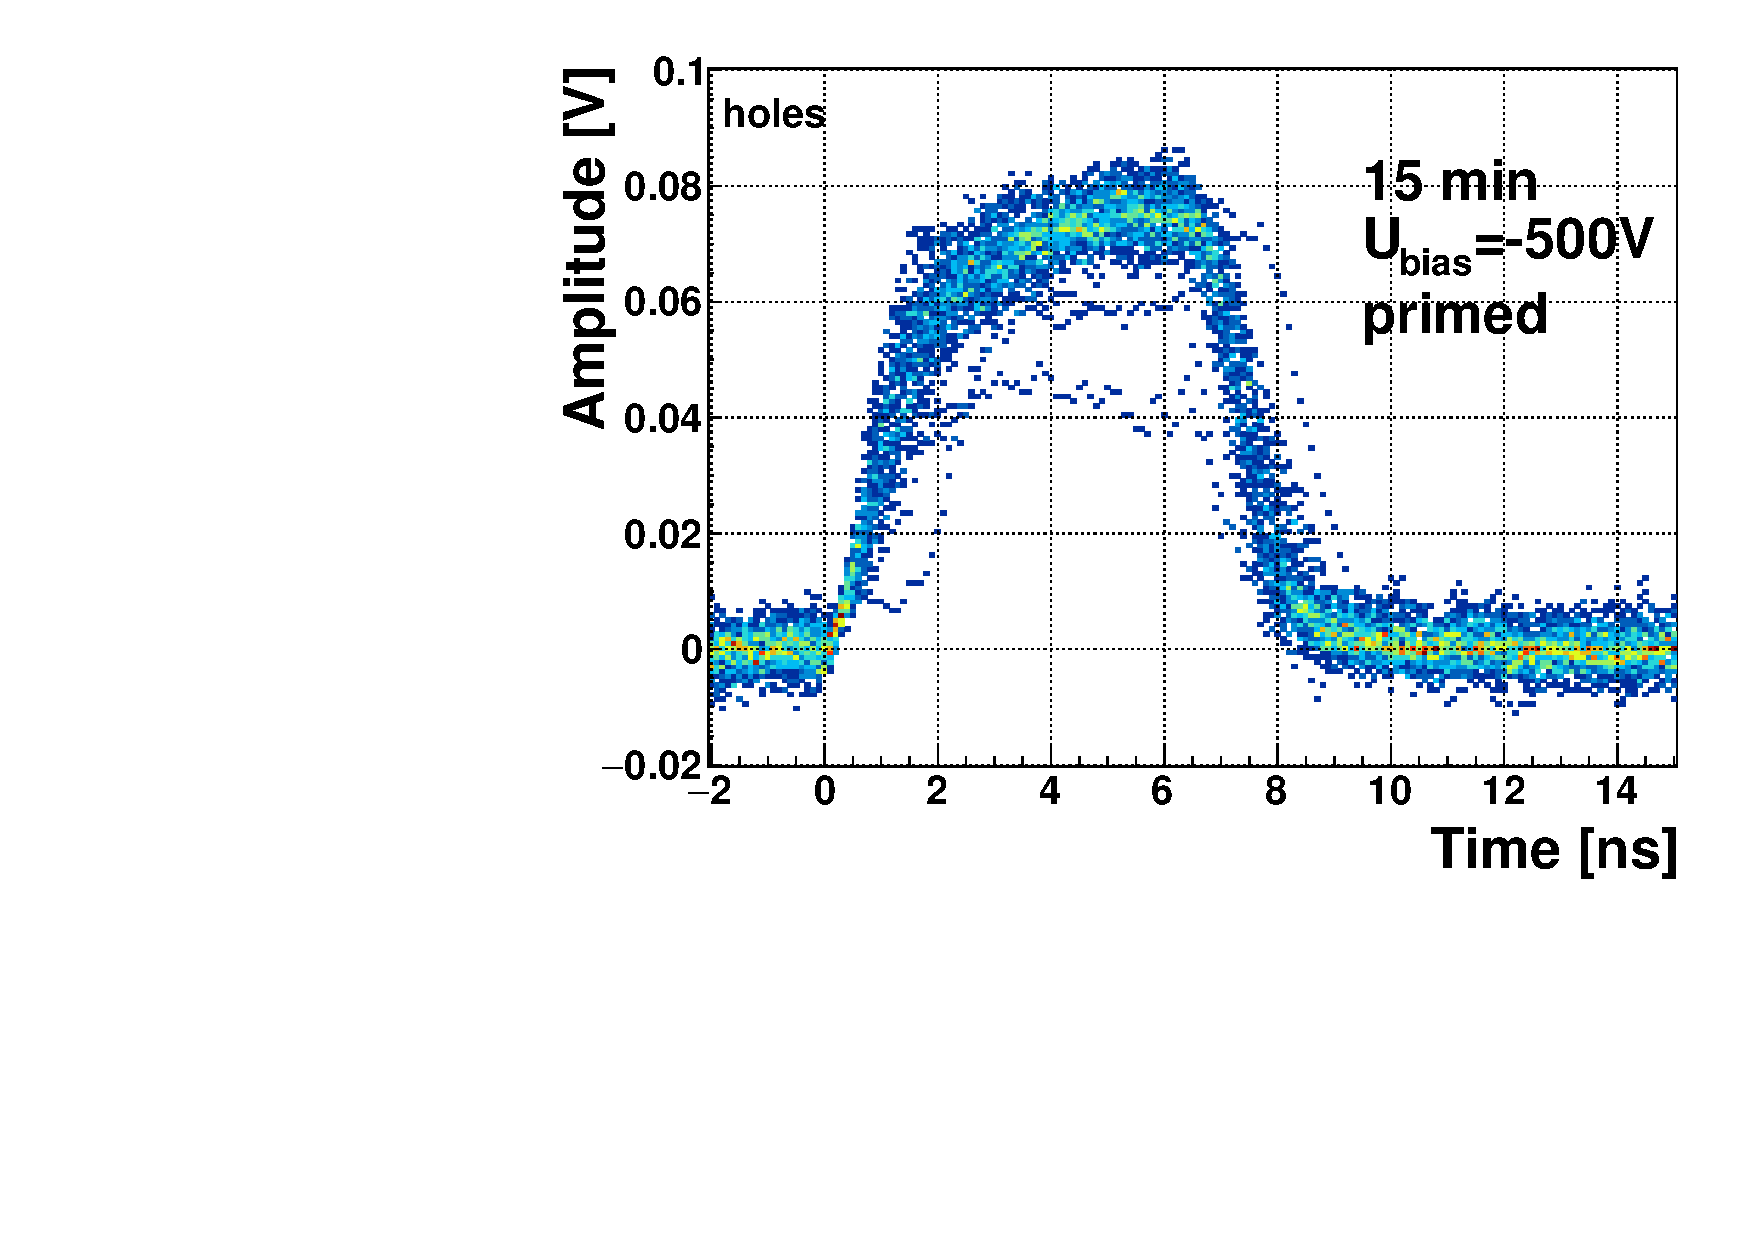
\includegraphics[width=0.47\textwidth]{03_measurement_results/scripts/plots/plotLifetime/holes15}  \label{fig:holes15lt}} \\
\subfloat{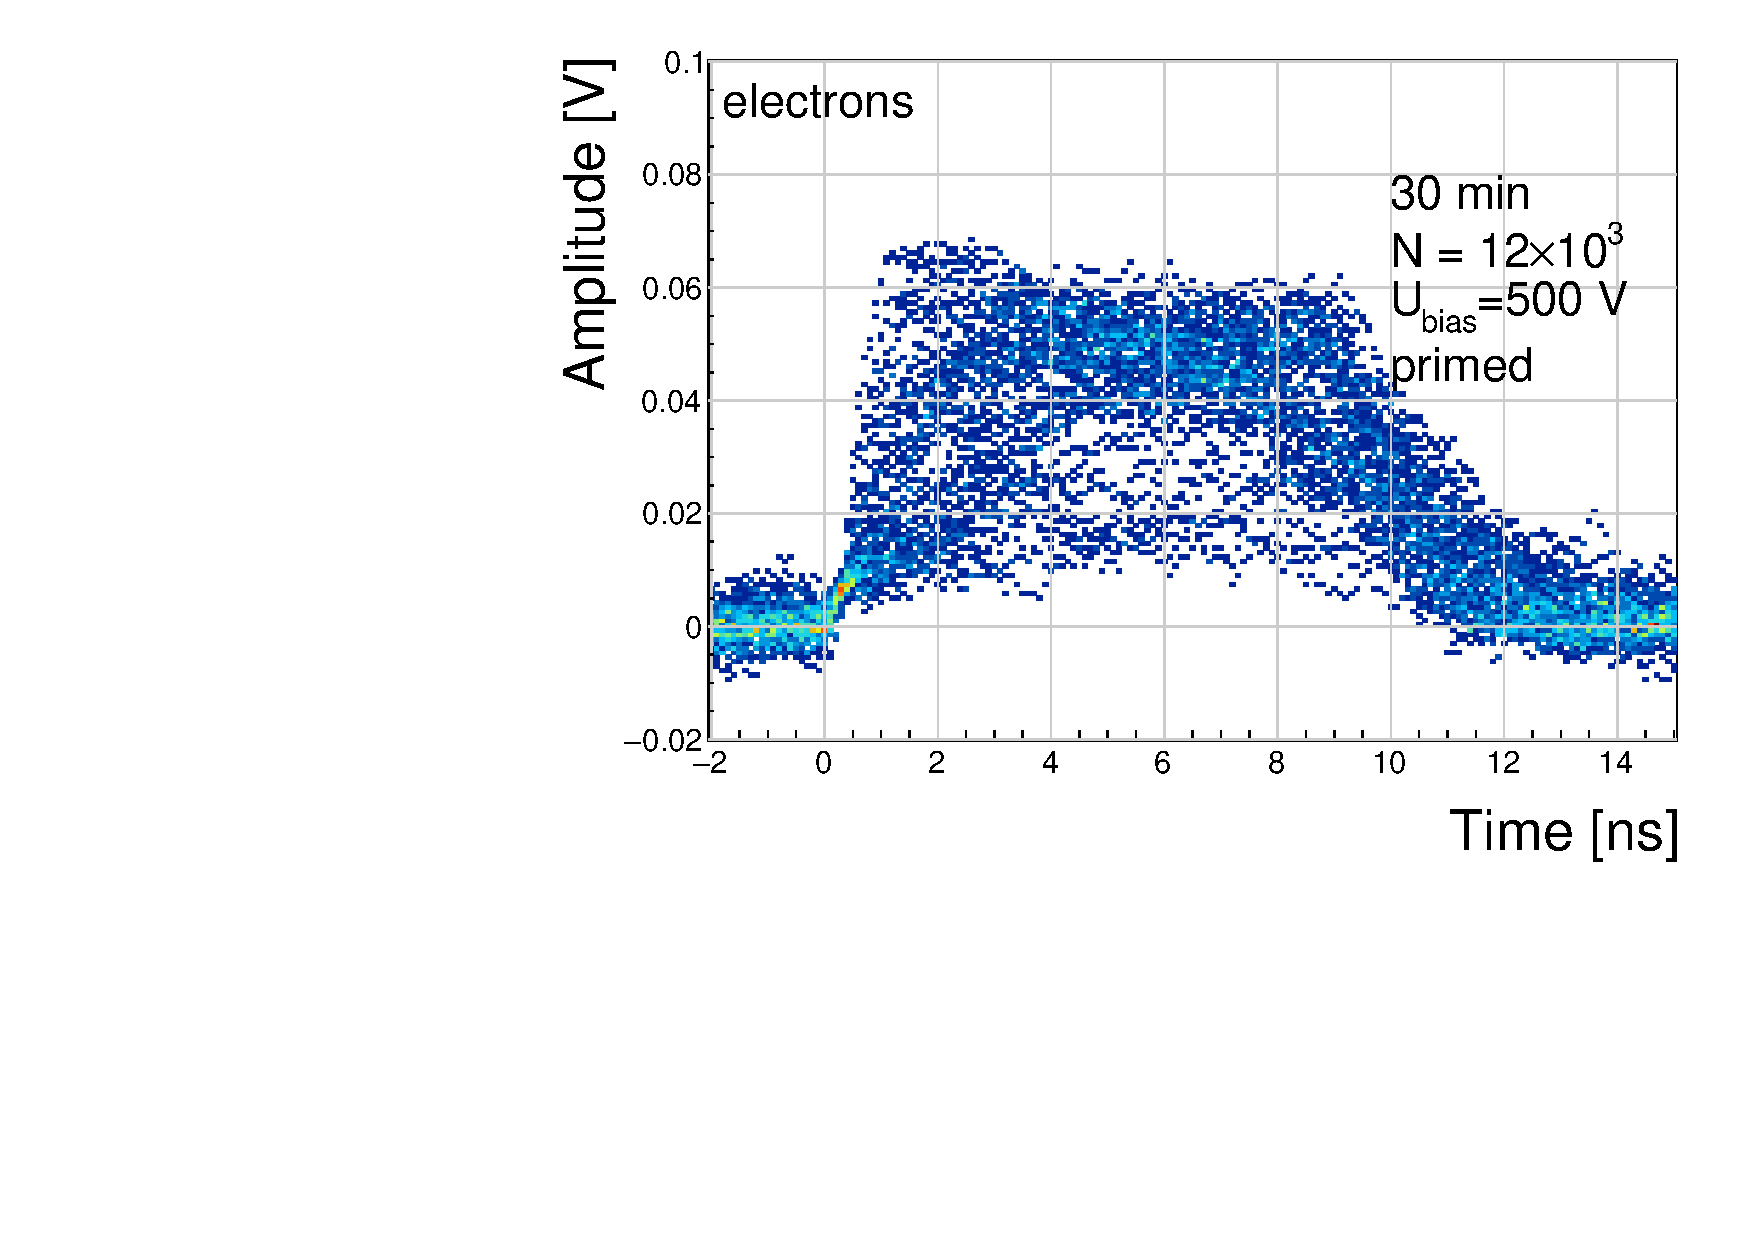
\includegraphics[width=0.47\textwidth]{03_measurement_results/scripts/plots/plotLifetime/elecs30}  \label{fig:elecs30lt}} &
\subfloat{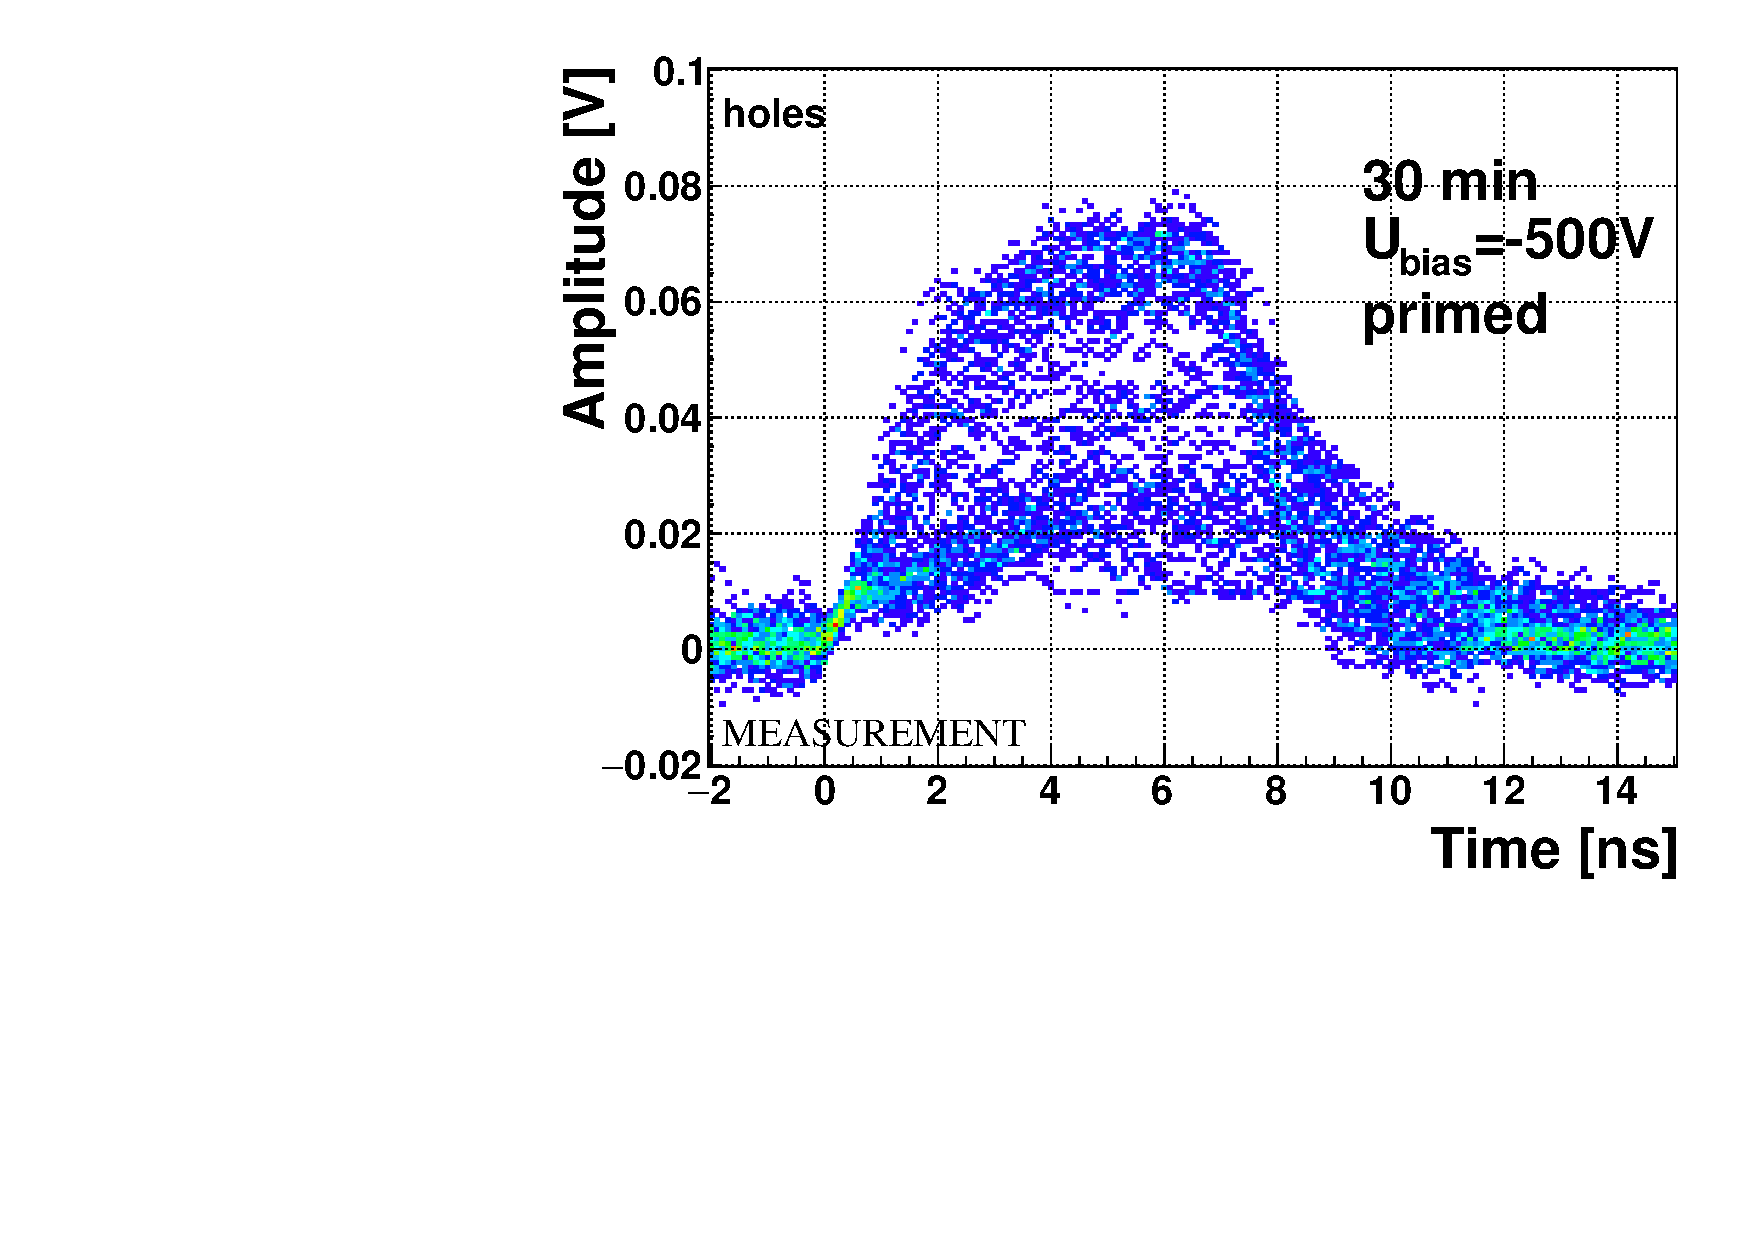
\includegraphics[width=0.47\textwidth]{03_measurement_results/scripts/plots/plotLifetime/holes30}  \label{fig:holes30lt}}
\end{tabular}
\caption{The signal of the irradiated and primed S79 deteriorates with time for both polarities. Every plot contains 60 superimposed pulses.}
\label{fig:lifetimeelecsholes}
\end{figure}

A more dedicated analysis of the first observation has been carried out as follows: at the beginning of the test when the diamond is still operating stably, 60 pulses are recorded. An average pulse is calculated. This is a \emph{reference pulse} for the subsequent measurement points.
% and plotted overlapped into a 2D histogram. An average pulse is extracted from this 2D distribution. 
Then an RMS of the individual pulses $\sigma_{n}$ with respect to the reference pulse is calculated and the resulting RMS values are summed together into $\sigma (0)$ and divided by the number of summed values:
\begin{equation}
\label{eq:sigmaref1}
\sigma (0) = \frac{\sum_\mathrm{n=1}^{60}\sigma_{n}}{60}.
\end{equation}

All the subsequent data points also consist of a set of 60 pulses. At every data point the summation of the RMS values of the individual pulses with respect to the reference pulse $\sigma (0)$ is calculated according to equation~\ref{eq:sigmaref1}. The ratio between the reference $\sigma (0)$ and discrete values $\sigma$ gives a measure of the change of the pulse shape with respect to the reference pulse at the start of the measurement. Therefore the initial value is 1 and it decreases if the RMS values of subsequent data points are higher.
%, the shape correlation $Corr_{\mathrm{shape}}$ is calculated:
%\begin{equation}
%\label{eq:correlation}
%Corr_{\mathrm{shape}} (t) = \frac{\sigma (0)}{\sigma} = \frac { \sum_\mathrm{x} \sum_\mathrm{y} w_{\mathrm{ref}}\cdot ( y_{\mathrm{avg}} - y_{\mathrm{ref}})^2 } { \sum_\mathrm{x} \sum_\mathrm{y} w\cdot ( y_{\mathrm{avg}} - y)^2 },
%\end{equation} 
%where $y_{\mathrm{avg}}$ is the amplitude of the current averaged pulse at time $x$, $y_{\mathrm{ref}}$ is the amplitude of the initial averaged pulse at time $x$, $y$ is the amplitude of the superimposed pulses in the 2D histogram and $w$ and $w_{\mathrm{ref}}$ are weights for the superimposed pulses for the current data point and the initial data point.
Figure~\ref{fig:longtermc2corr} shows the ratio $\frac{\sigma (0) }{\sigma(\Phi)}$. From the data obtained it can be concluded that the initial pulse shape quickly starts deteriorating. In fact, the deterioration of the shape follows an approximate exponential decay function before it settles at the lowest value. The resulting decay constants for electrons and holes are $\tau_{\mathrm{e}}=(4400\pm150)$~$\upalpha^{-1}$ and $\tau_{\mathrm{h}}=(3300\pm140)$~$\upalpha^{-1}$. The electrons retain the initial shape for longer. The deteriorated shapes also seem to be for a factor of 2 better than those of the holes. 

\begin{figure}[!t]
\begin{center}
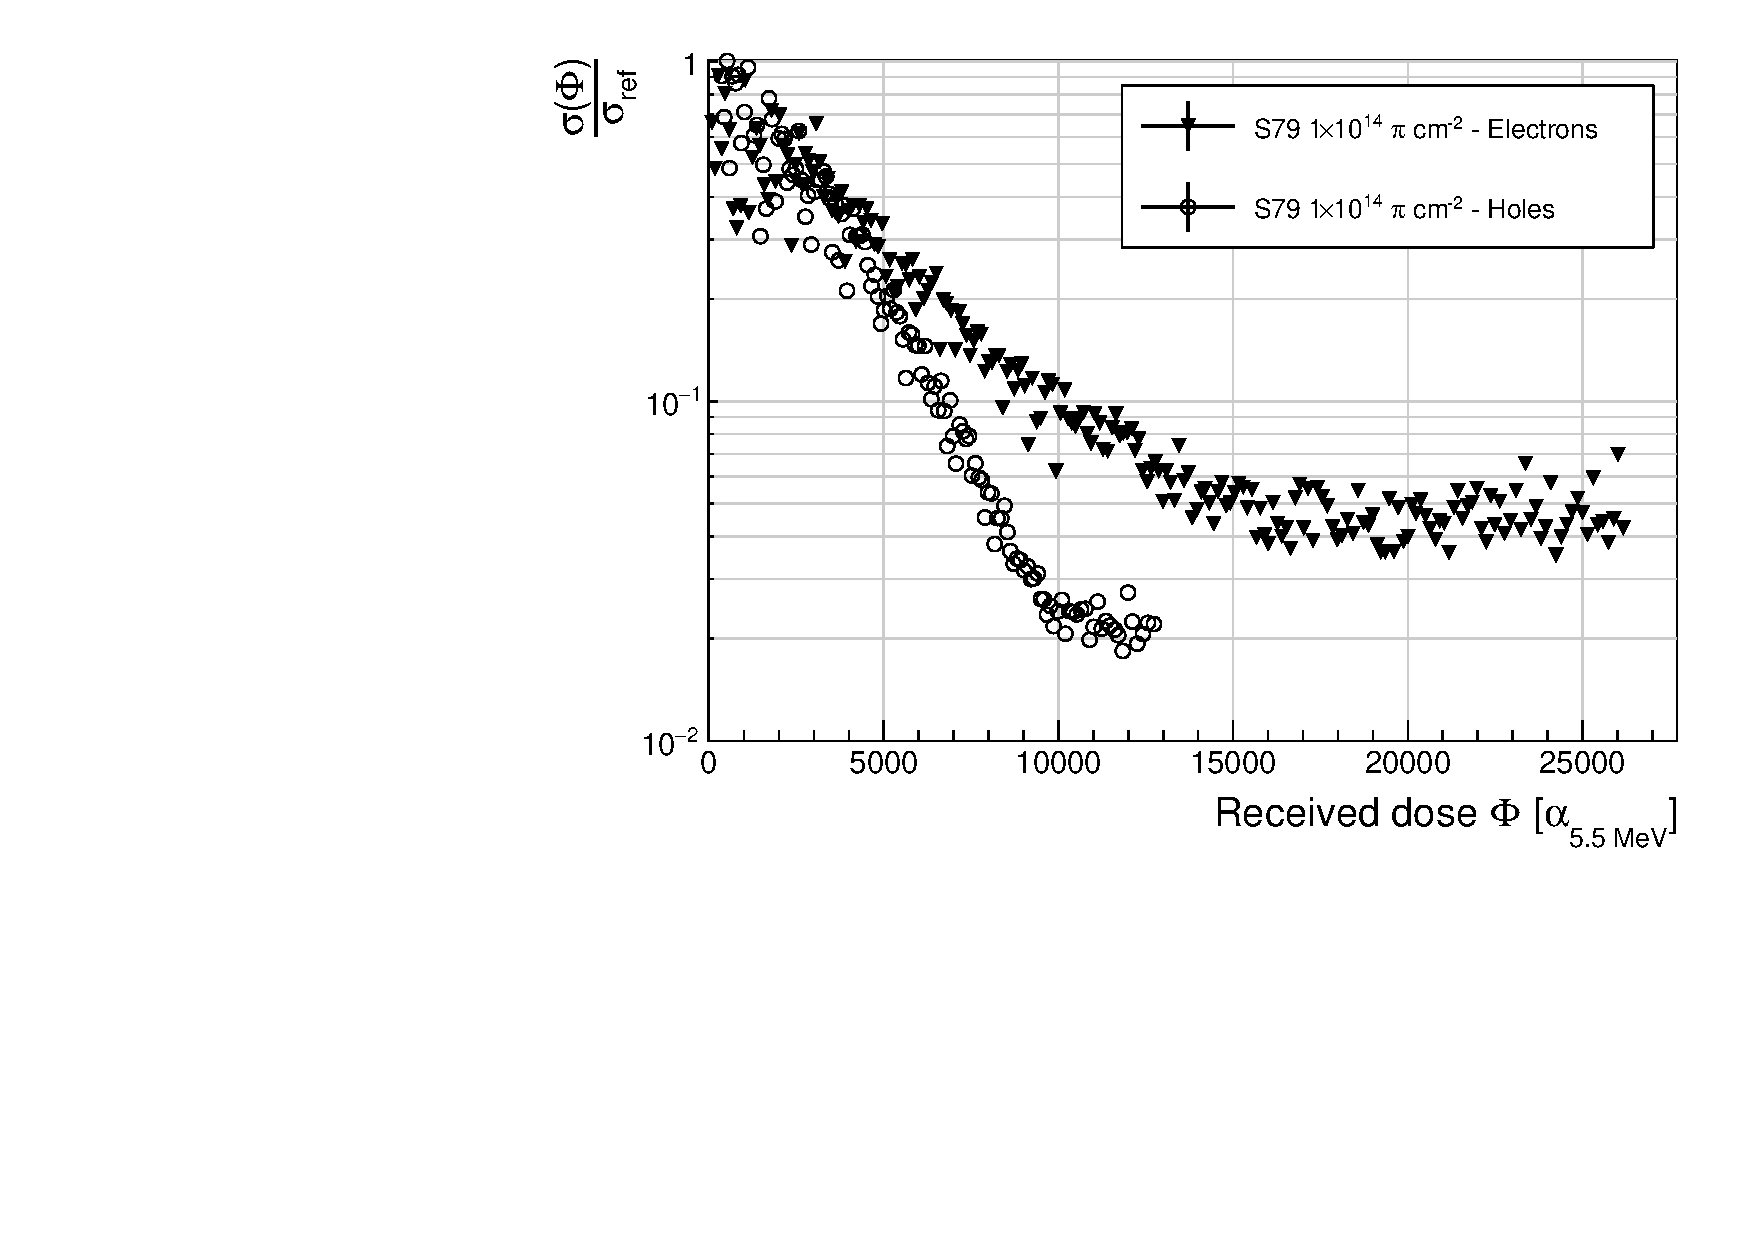
\includegraphics[width=0.7\textwidth]{03_measurement_results/scripts/plots/plotLifetime/corrlifetime}
\caption{Deterioration of the pulse shapes with time.}
\label{fig:longtermc2corr}
\end{center}
\end{figure}


%DISCUSSION!!!
%Since only one charge flavour is drifting through the bulk whereas the other is quickly recombined, this already determines the imbalance in spatial distribution of trapped charges. 
%MOVE TO THE DISCUSSION!
\begin{description}
\item[Discussion] 

One hypothesis is that this behaviour is caused by space-charge build-up. Charge carriers get stopped in the charge traps in the bulk for a long time, building up regions of space-charge. The built up space-charge creates an internal electric field -- polarisation. This field in turn affects the speed of the drifting charge carriers. Since the movement of the carriers is inducing the electric current, the field gradient can be observed in the current signal. The fact that the signal shapes vary significantly might be due to a very non-uniform electric field, suggesting a complex polarisation in the sensor.
%$\upalpha$ affect the irradiated diamond differently than when subjected to $\beta$ radiation. This can be due to several contributions:
%\begin{description} 
%\item[Quantity of deposited energy.] The deposited energy on its path produces 24 times more e-h pairs than that of a MIP, according to equations~\ref{eq:qBeta} and~\ref{eq:qAlpha}. Such a difference may affect the charge collection efficiency due to saturation.
%\item[A point-like charge carrier creation.] The energy of an $\upalpha$ particle is deposited in a small volume -- 14~$\upmu$m in depth and $\sim$20~nm radially~\cite{Jansen:1956431}. A dense distribution of charge carriers  might affect their behaviour at the start of the drift.
%\item[Single-polarity charge carriers.] Carriers of only one polarity drift through the sensor while those of the opposite polarity almost instantly reach the adjacent electrode. Therefore the charges only one polarity get trapped along the drift path, contributing to a single-polarity space-charge build-up.
%\end{description}
\begin{figure}[!t]
\begin{center}
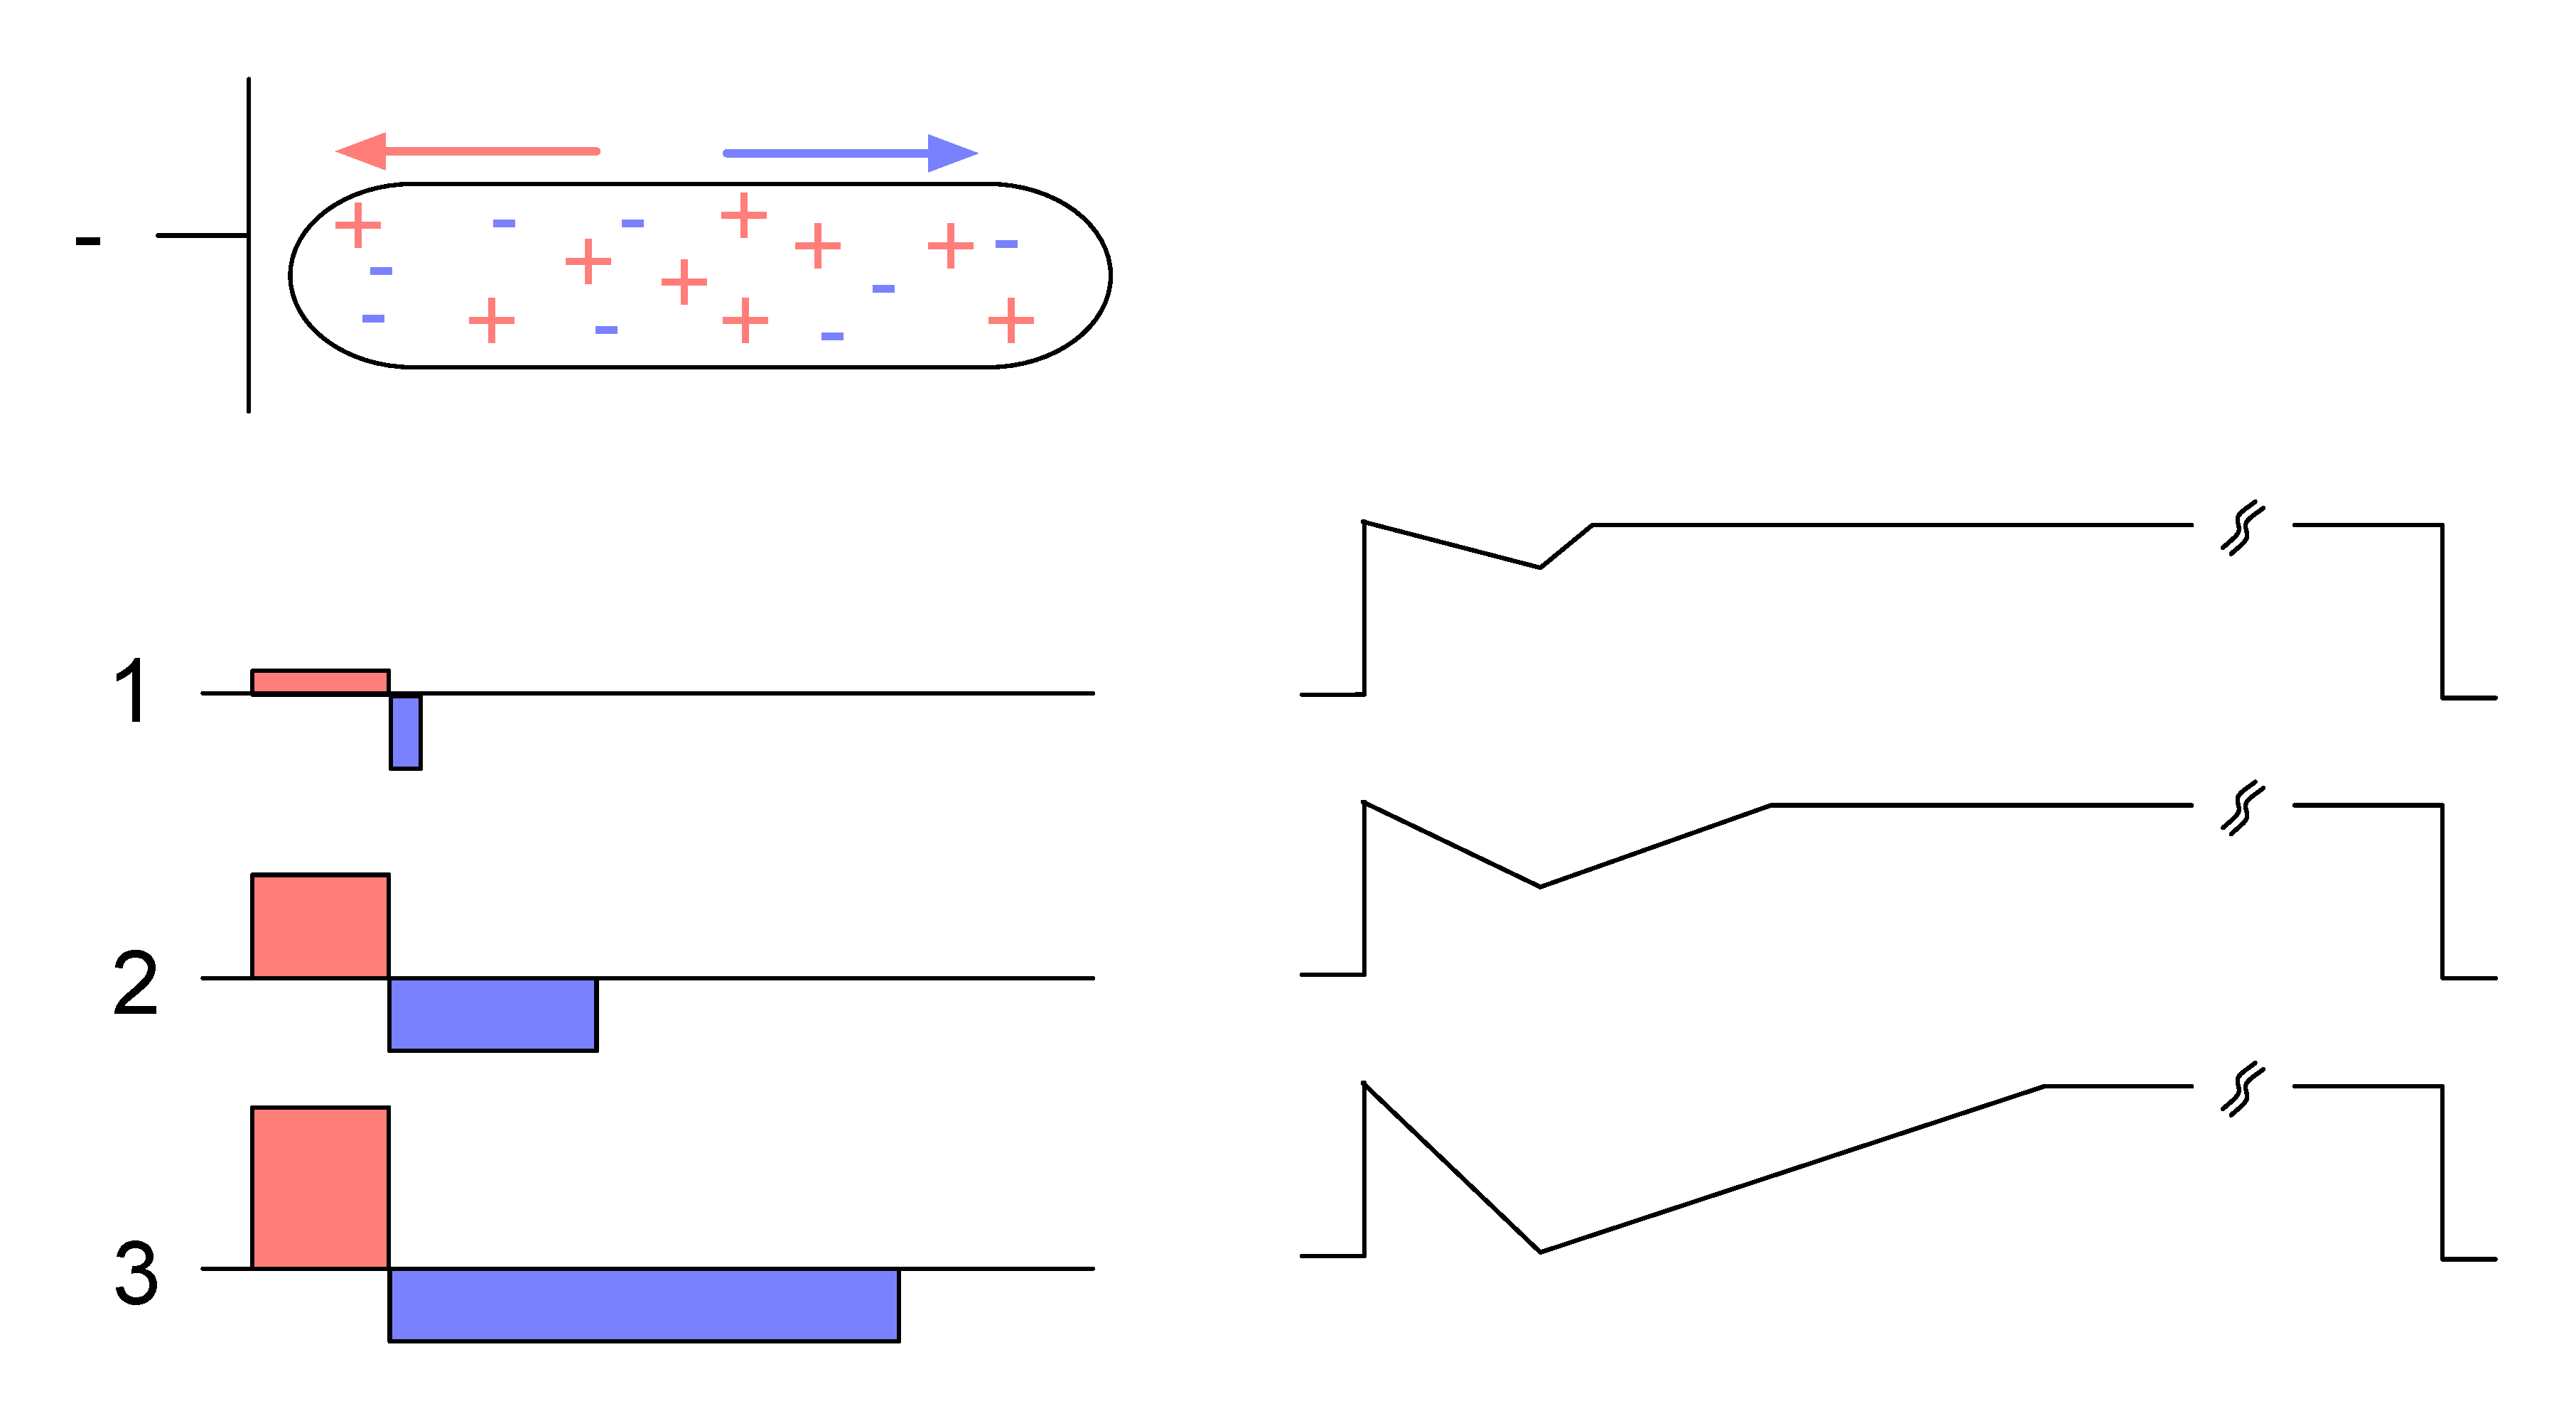
\includegraphics[width=0.4\textwidth]{03_measurement_results/plots/elfield}
\caption{Space-charge build-up at the electrode. The figure shows the $\sim$15~$\upmu$m long charge cloud that is created by an $\upalpha$ particle. The positive charge carriers get trapped in charge traps in the damaged surface at the electrode. The positive space charge attracts the negative carriers, which form a negative space charge region. Both regions gradually grow, eventually creating a barrier in the electric field distribution, as shown on the right side of the diagram.}
\label{fig:elfield}
\end{center}
\end{figure}

Figure~\ref{fig:elfield} shows how the space-charge might be built up at the entry point of the $\upalpha$ particle. The assumption is that the first few~$\upmu$m of diamond surface are significantly more damaged than the rest of the material. Therefore the probability that charge carriers would get trapped at the edge of the sensor is higher. If the sensor is biased as shown in the figure, the positive charge cloud drifts towards the adjacent electrode while the negative cloud drifts through the sensor to the opposite one. Therefore most of the trapped carriers at the adjacent electrode are positive, forming a strong positive space-charge barrier in the first few $\upmu$m of the sensor (1). The negative carriers created by subsequent $\upalpha$ particles are attracted by the positive space charge and get trapped close to the positive space-charge (2). This negative space-charge region is gradually stretched inwards (3). Together the two regions form a barrier which counteracts the externally applied electrical field. Such a distortion of the field prevents the charge carriers from drifting freely within the space-charge region. Only those negative carriers that diffuse through this barrier can start drifting towards the positive electrode. Others either recombine or are trapped, contributing to the build-up of the barrier. 

This hypothesis explains the gradual loss of collected charge in figure~\ref{fig:longtermcx} and the pulses with a slow rising edge in figures~\ref{fig:lifetimeelecsholes}. However, this simple picture cannot explain the electron pulses with a negative slope. Further reading regarding the space-charge build-up is available in~\cite{Eremin2002537,	4327634, s150613424}, however, no direct explanation of the observed phenomenon has been given.

%The charge carriers are created in a small volume whereby some immediately get trapped, some recombine to form excitons~\cite{PHSEM:00000} and others start drifting. The remaining charge carriers drift towards their respective electrodes. Both are trapped on their way, causing the space-charge build-up of one polarity on the first 14~$\upmu$m and of the other polarity all along the sensor thickness. A resulting electric field is very non-uniform, which explains the unstable current pulses. 
\end{description}







\begin{description}
\item[Restoring the pulse shapes] Finally, an effort has been made to find a way for the pulse shapes to return to their initial state. Five methods are listed: 
\begin{enumerate}[itemsep=0.1\baselineskip]
\item No source, with bias voltage, 
\item No source, without bias voltage, 
\item Priming with $\upgamma$ at a rate of 400~s$^{-1}$cm$^{-1}$ without bias voltage, 
\item Priming with $\upbeta$ at a rate of $1'000$~s$^{-1}$cm$^{-1}$ with bias voltage and 
\item Priming with $\upbeta$ at a rate of $1'000$~s$^{-1}$cm$^{-1}$ without bias voltage. 
\end{enumerate}
Before starting each method, the diamond sample S79 is first primed using a $^{90}$Sr source for approximately one hour. Then the bias voltage is switched on and an $^{241}$Am source is put on top. The pulses produced by the incident $\upalpha$ particles have a proper rectangular pulse at the beginning, but then start changing -- first gradually and later increasingly more in an erratic way, as described in the text above. After approximately 30~minutes, one of the methods is tested. When a ``healing'' procedure is started, a set of 60~pulses is taken at irregular points of time to observe the change in the pulse shape and to assess the quality of the ``healing'' procedure. Then the bias voltage is switched off and the sample is primed again to reset its state before starting the next measurement. 

The results depicted in figure~\ref{fig:formCorr} show that the methods (3) and (5) improve the shape, method (2) helps slowly, (1) does not show any change with time and (4) at first improves, but then significantly degrades the shape. The effect observed in method (4) has already been described in~\cite{Kramberger:2013wva}. The ``healing'' process therefore depends on the rate of radiation, the bias voltage and the time of exposure. The ionising radiation creates free charges, which quickly recombine close to the place of generation. It is likely that they also release the charges trapped during the measurement, reducing the overall effect of the space-charge. The traps get filled with both flavours of carriers, thus they are neutralised. The pulse shape gradually returns to its initial state.

\begin{footnotesize}
\begin{center}
\begin{tabular}{   c  c  c  c c }
\hline
Procedure & Source & Type of radiation & Bias voltage & Effectiveness \\
\hline
1 & /                   & /                 & ON    & no \\
2 & /                   & /                 & /        & slow \\
3 & $^{60}$Co   & $\upgamma$ &/         & YES \\
4 & $^{90}$Sr    & $\upbeta$      & ON    & no \\
5 & $^{90}$Sr    & $\upbeta$      & /         & YES \\
\hline
\end{tabular}
\captionof{table}{Effectiveness of healing procedures.}
\label{tab:healing}
\end{center}
\end{footnotesize}

\begin{figure}[!t]
\begin{center}
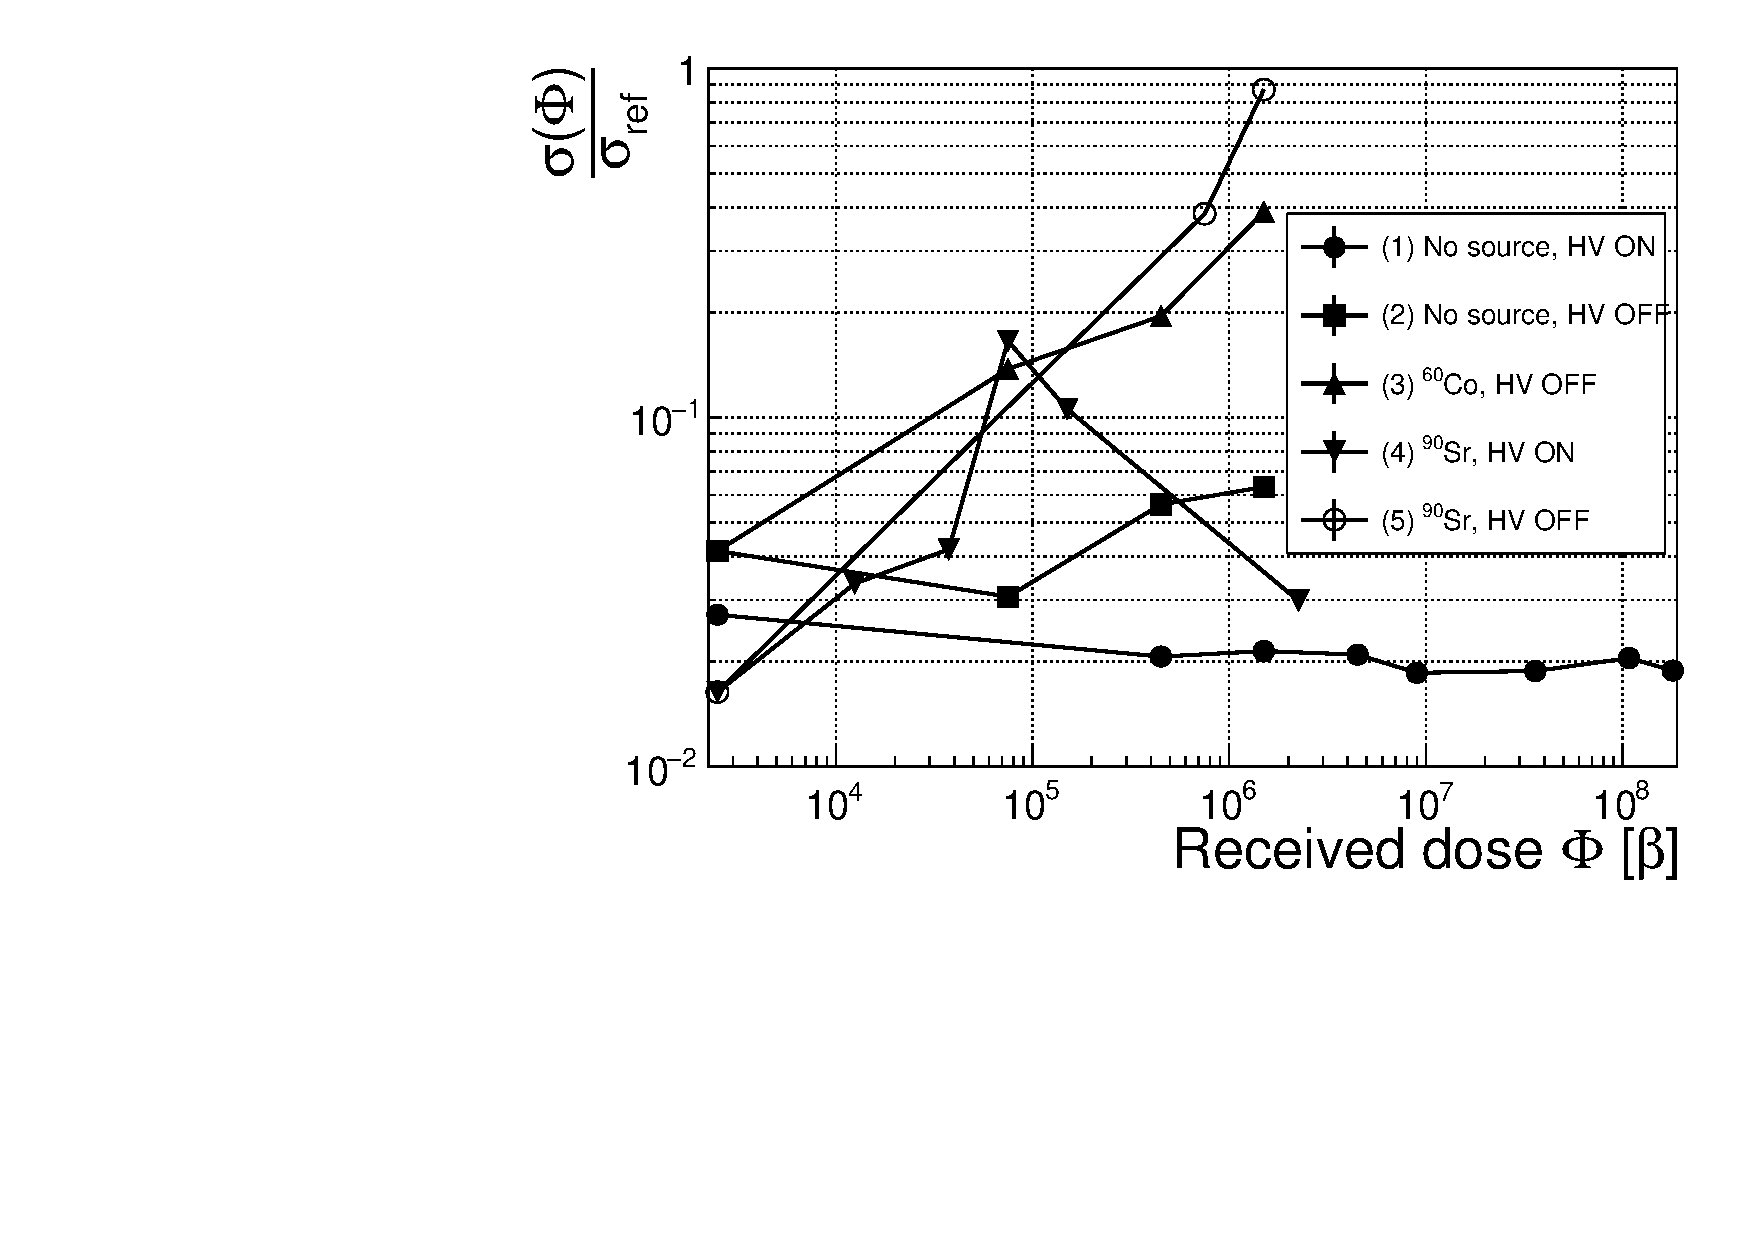
\includegraphics[width=0.7\textwidth]{03_measurement_results/scripts/plots/plotLifetime/formCorrelation}
\caption{Comparison of the five procedures for the ``healing'' process for an irradiated diamond that had been exposed to $\upalpha$ radiation with a rate of $7$~s$^{-1}$, with the bias voltage switched on, for at least 30~minutes.}
\label{fig:formCorr}
\end{center}
\end{figure}

%TO-DO conclusions: limitations

\item[Summary] The shape of the pulses caused by $\upalpha$ radiation changes with time for irradiated samples. The shape of the pulses gets distorted. The charge collection decreases and its spread increases. The signal shapes are probably affected by a non-uniform electric field, which is caused by polarisation in the sensor. The signal degradation happens even faster for non-primed diamonds. To ``heal'' the diamond -- to bring the pulse shapes back to their initial shape -- the sample must be primed using a $\upbeta$ or a $\upgamma$ source for several minutes without bias voltage. Switching to the inverse polarity for a few seconds helps a bit, but in a long run distorts the signal, preventing it from returning to the initial shape.
\end{description}









% ---------------------------------------------------------------------------------------------------------------
\clearpage
\section{Temperature limitations}
\label{sec:templimit}
% ---------------------------------------------------------------------------------------------------------------
A test has been carried out to evaluate the effect of temperature on the output signal of the diamond sensors. A cryostat filled with liquid helium is used to cool down the sensor during the measurement process. The current signal response to $\upalpha$-particles is measured at 18 temperature points between 4~K and 295~K. At every temperature point a set of 300 pulses is recorded at a range of positive and negative bias voltages and averaged in the analysis.
%The resulting data show that the charge collection is stable from RT down to 150~K where it starts decreasing. It stabilises again at about one third of the initial value at 75~K. This behaviour was first measured and discussed by H. Jansen~\cite{Jansen:1956431}.

%\subsubsection{Acoustic phonon scattering}

%The positively charged hole and the negatively charged electron in the hole attract each other via the Coulomb force and may undergo a bonding process during which an exciton is emitted. 

%\subsubsection{Exciton formation and recombination}
%That phonon is referred to as \emph{exciton}~\cite{Exciton}. 

 %figures~\ref{fig:chgtempelecs} and~\ref{fig:chgtempholes}.


%The irradiated samples were put in the cryostat, which was cooled down to 4.2~K using liquid helium. TCT data were then taken at a range of bias voltages at temperature points ranging between 4.2~K and room temperature (RT). The results showed that irradiation causes forming of charge traps in the bulk.l;'
%
%TO-DO: get the Tau and plot it against T. 
%TO-DO: plot the drift time against square voltage.


\subsection{Temperature-variant $\upalpha$-TCT before irradiation}
% Show a set of pulses
Three sCVD diamond samples have been tested at a range of temperatures using the $\upalpha$-TCT technique to verify the consistency of the results with those obtained by H. Jansen in~\cite{Jansen:1956431}. 

The resulting averaged pulses of the non-irradiated sample S52 at the 260~K temperature point and a bias voltage of $\pm$700~V, $\pm$500~V and $\pm$400~V are shown in figure~\ref{fig:voltpulse}. The pulses induced by positive charge carriers are shorter than those induced by electrons, which means that holes travel faster in diamond. The area of the pulse, however, is the same for both polarities, which corresponds to the fact that the same amount of charge carriers is drifting in both cases.

\begin{figure}[!t]
\begin{tabular}{rr}
\subfloat{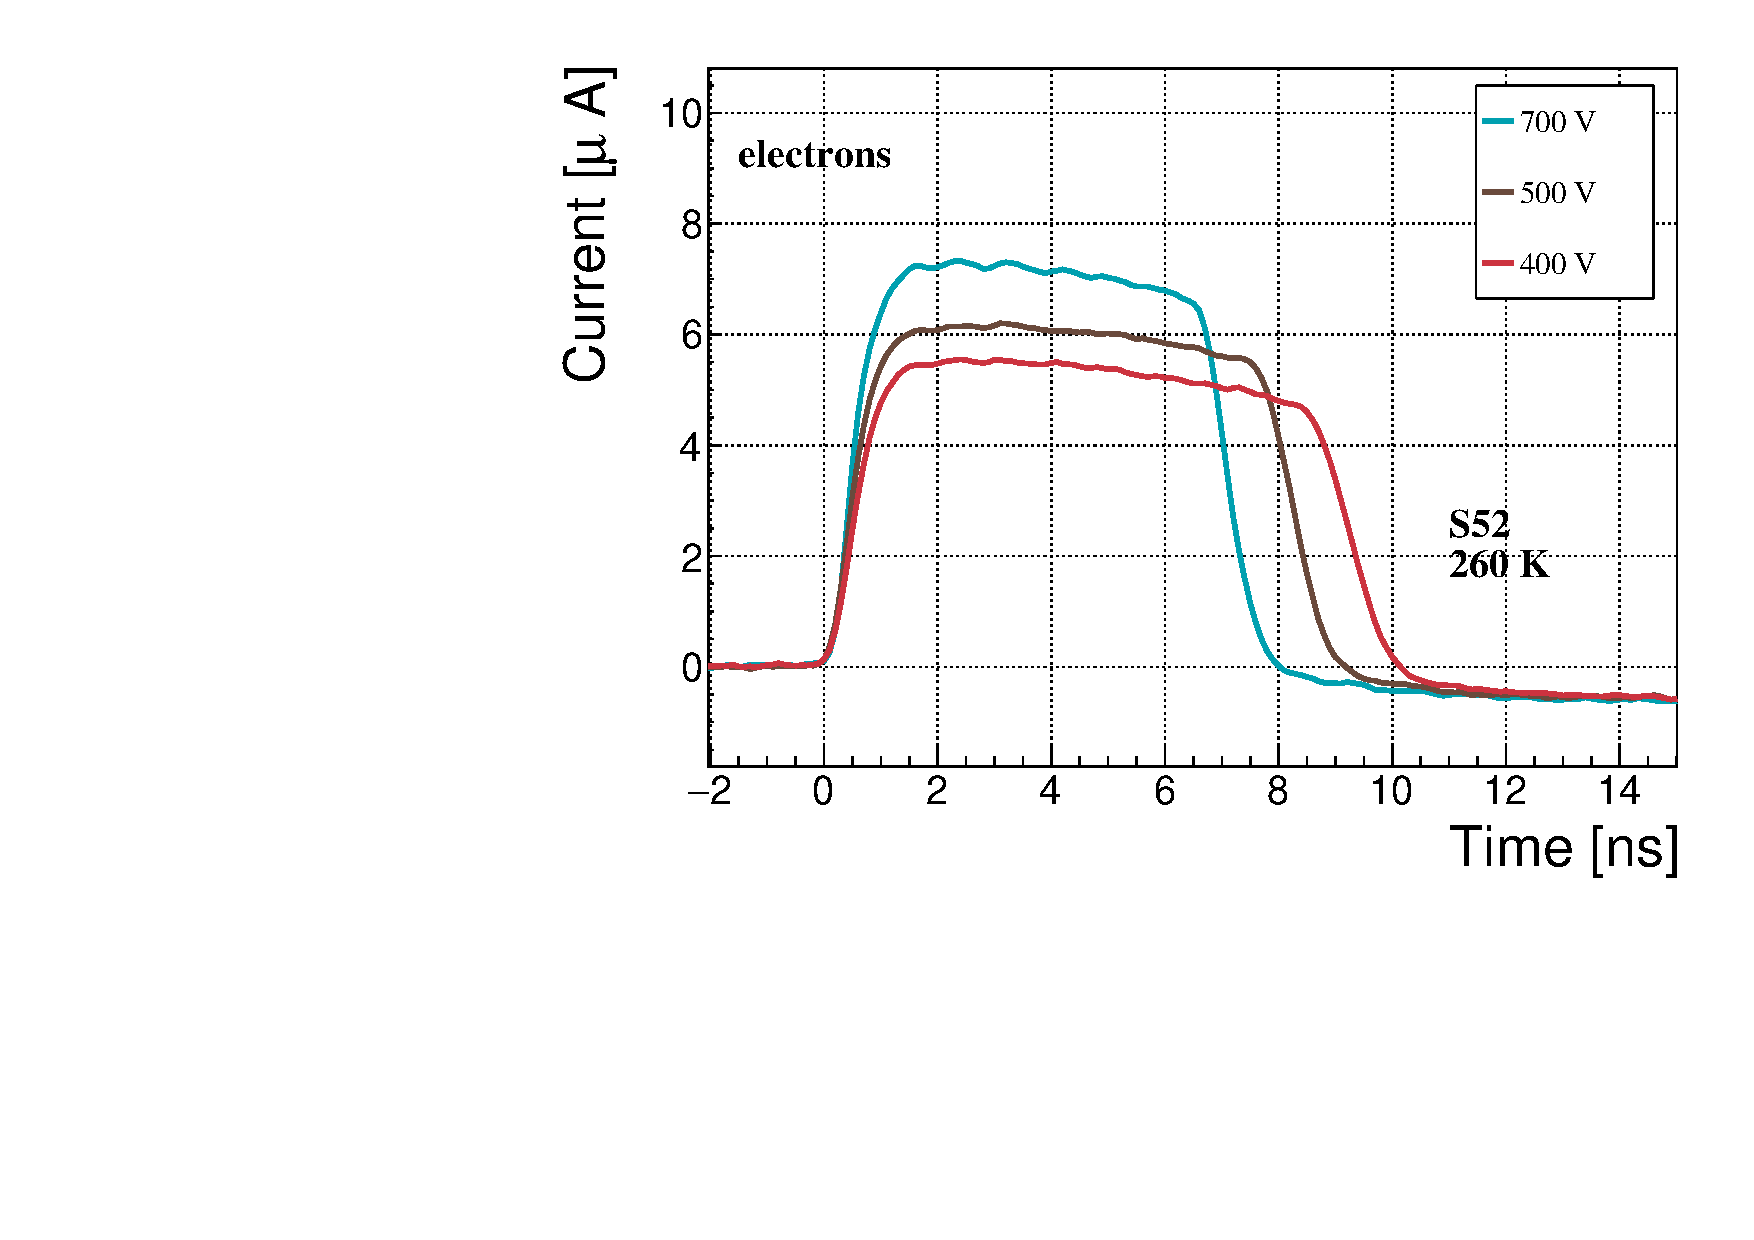
\includegraphics[width=0.47\textwidth]{03_measurement_results/scripts/plots/pulsesVolt/varVolt_S52_elecs_260k} \label{fig:S52cTplus}} &
\subfloat{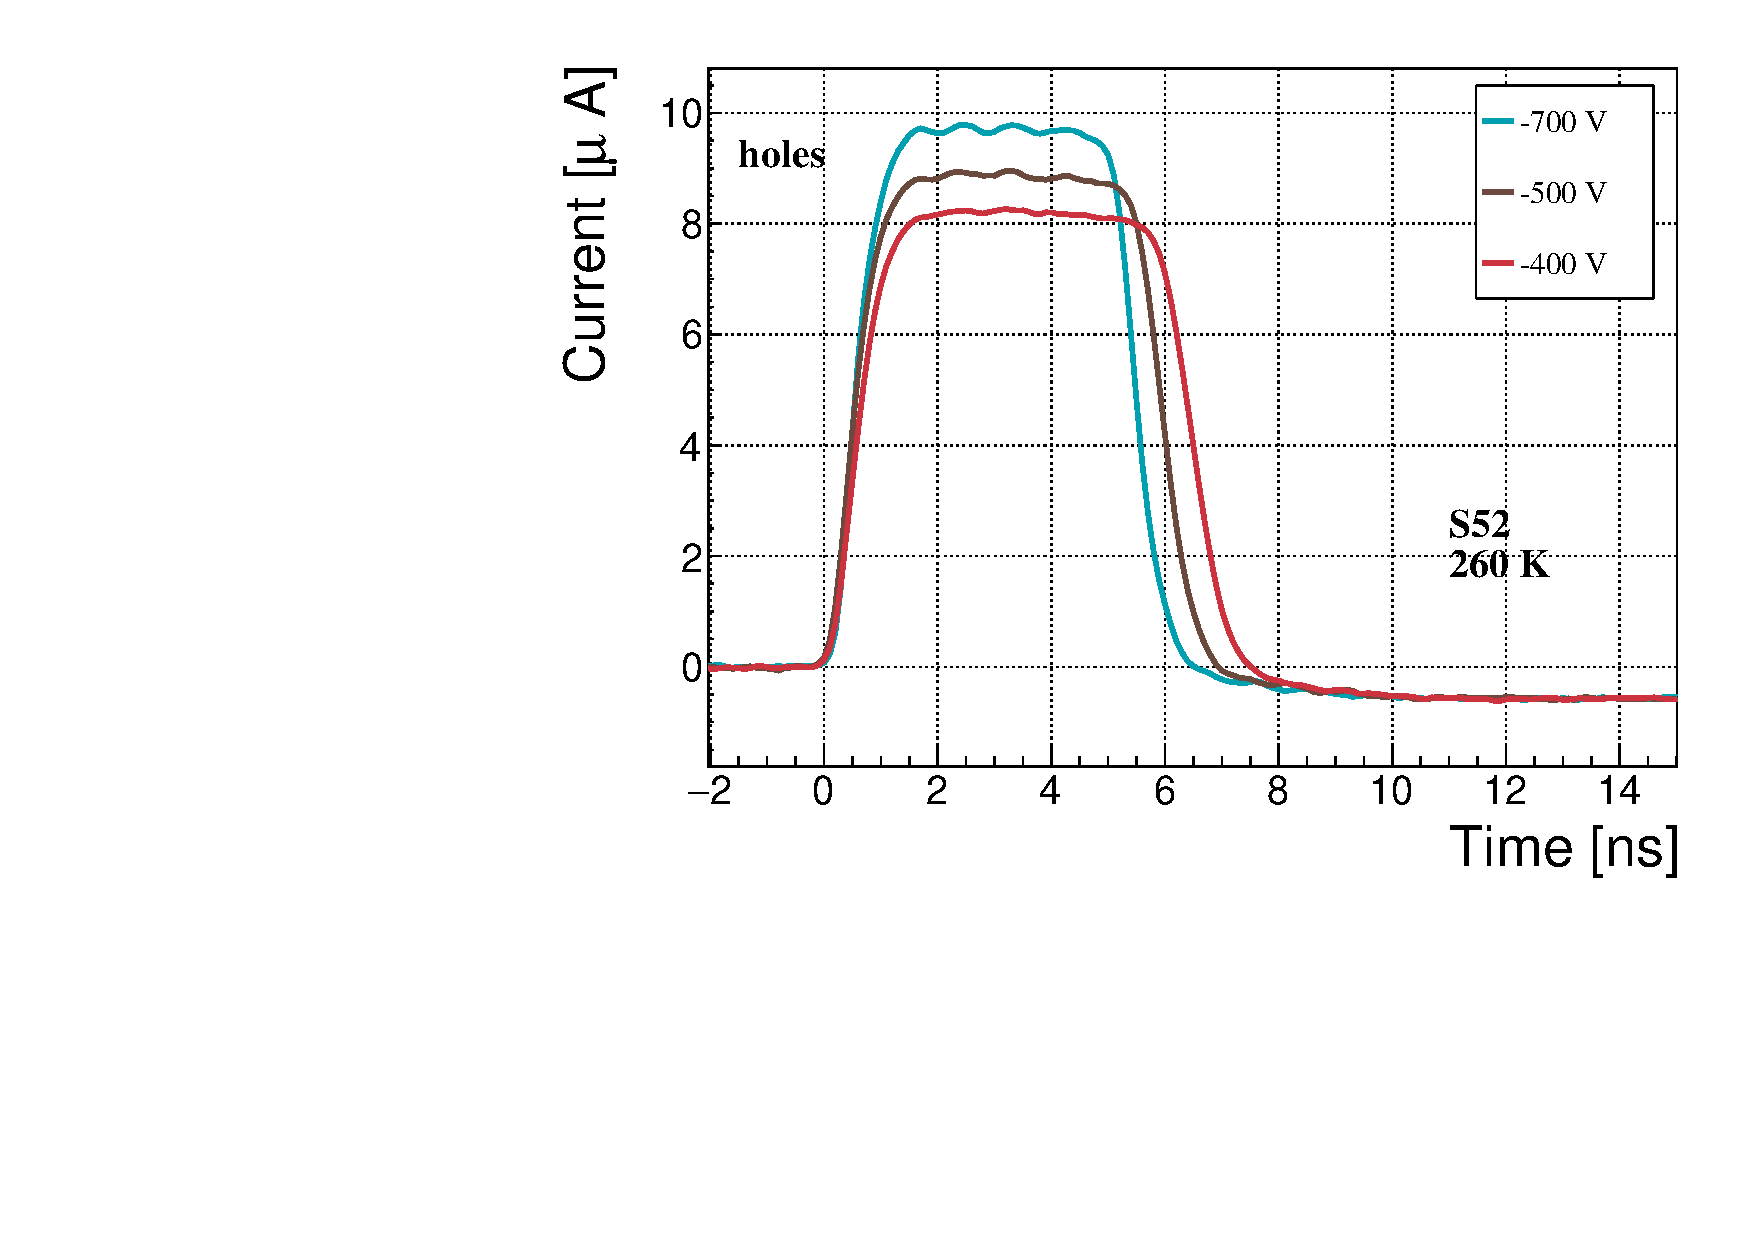
\includegraphics[width=0.47\textwidth]{03_measurement_results/scripts/plots/pulsesVolt/varVolt_S52_holes_260k}  \label{fig:S52ctTminus}}
\end{tabular}
\caption{Varied bias voltage at a fixed temperature of 260~K.}
\label{fig:voltpulse}
\end{figure}

\begin{figure}%[!t]
\begin{tabular}{rr}
\subfloat{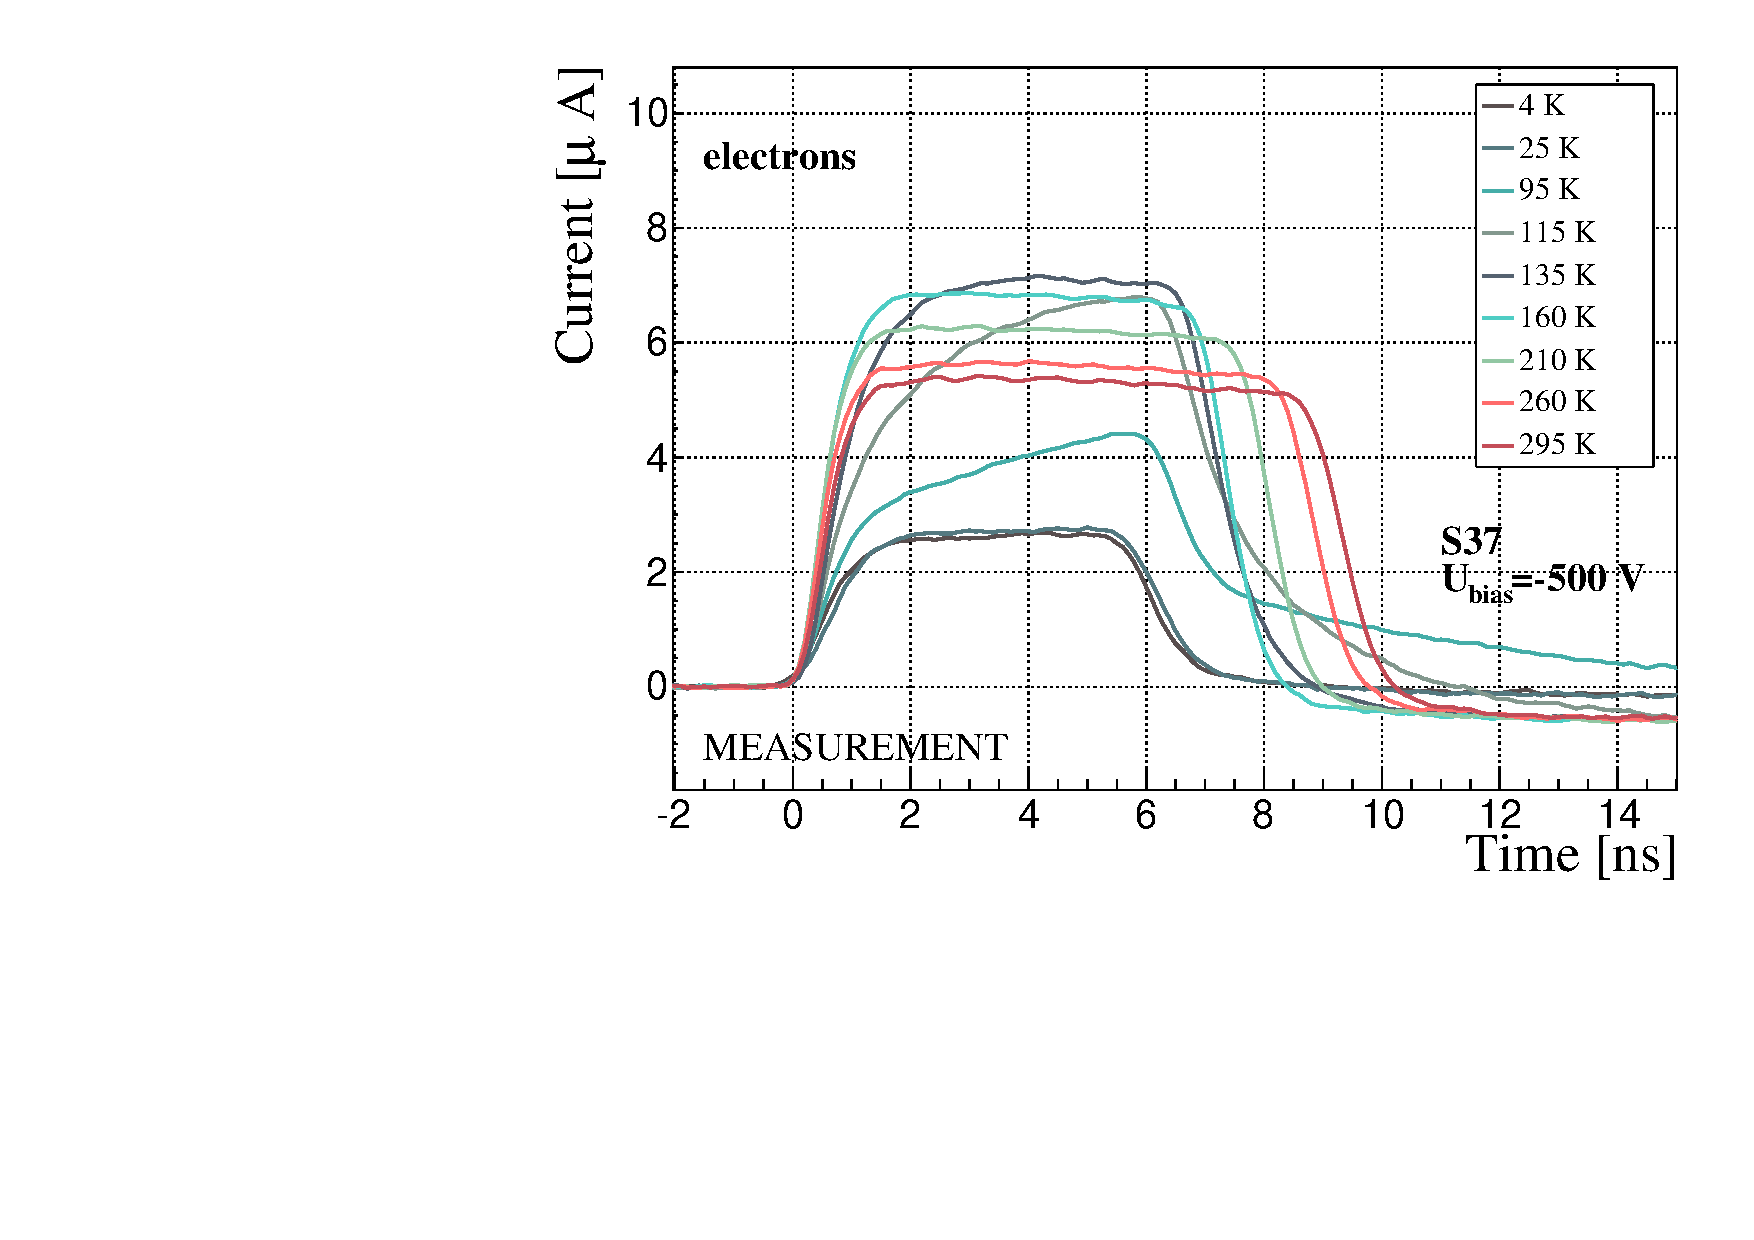
\includegraphics[width=0.47\textwidth]{03_measurement_results/scripts/plots/pulses/S37_elecs} \label{fig:S37plus}} &
\subfloat{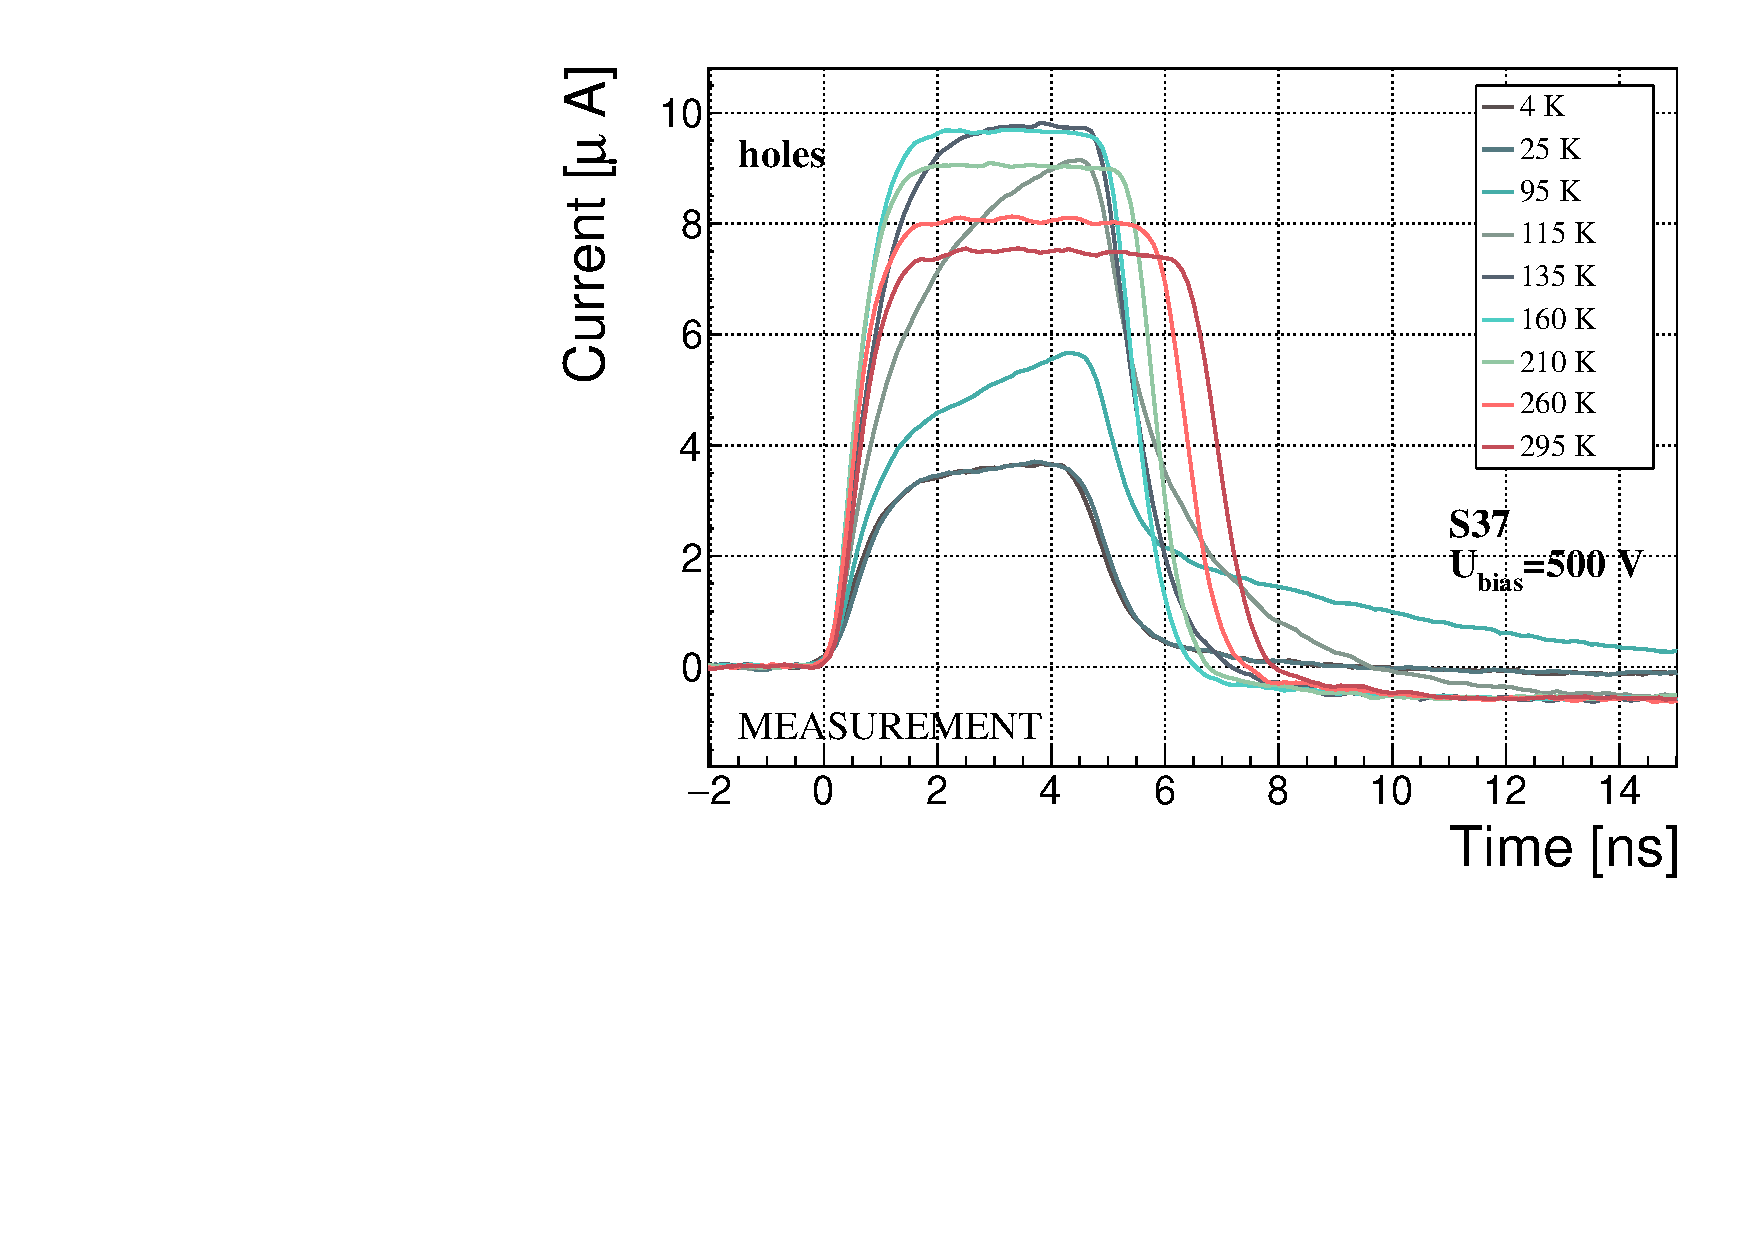
\includegraphics[width=0.47\textwidth]{03_measurement_results/scripts/plots/pulses/S37_holes}  \label{fig:S37minus}} \\
\subfloat{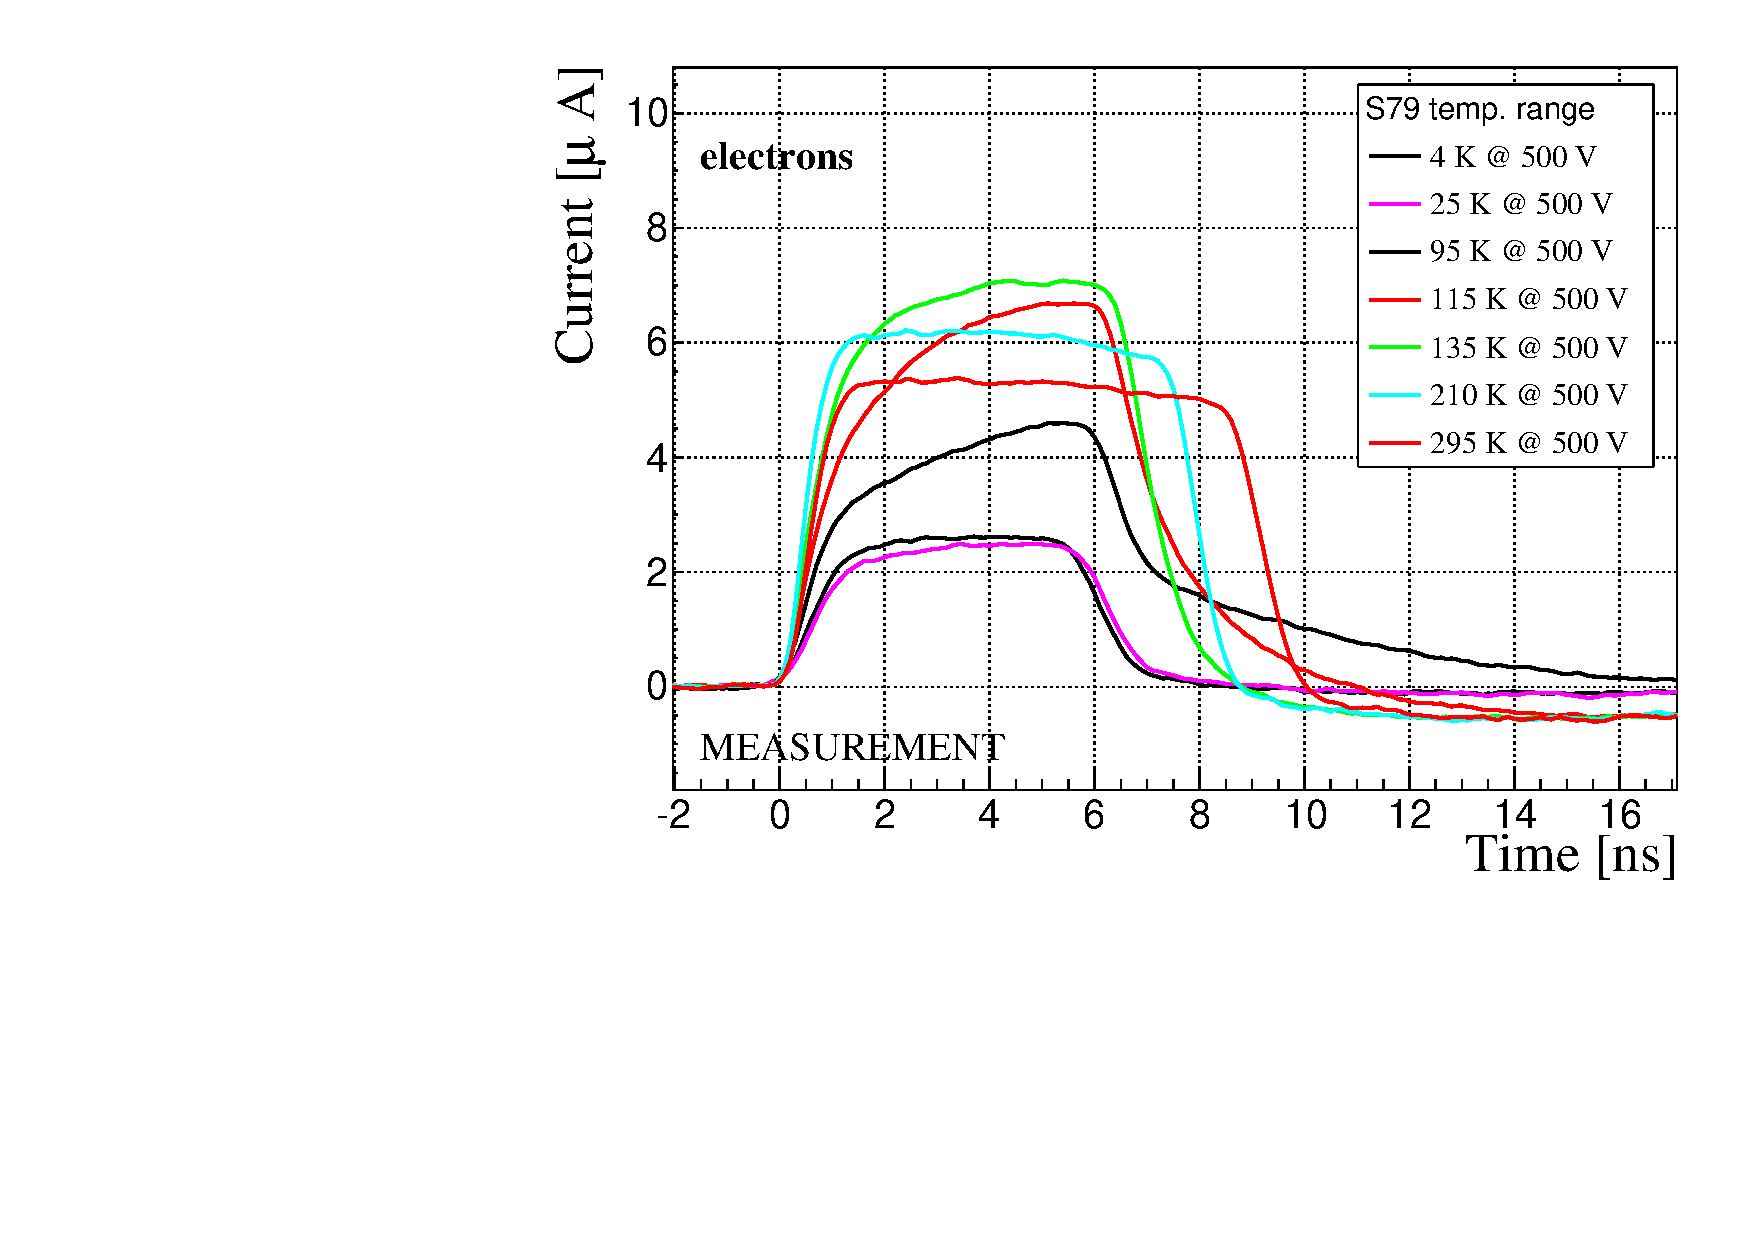
\includegraphics[width=0.47\textwidth]{03_measurement_results/scripts/plots/pulses/S79_elecs} \label{fig:S79plus}} &
\subfloat{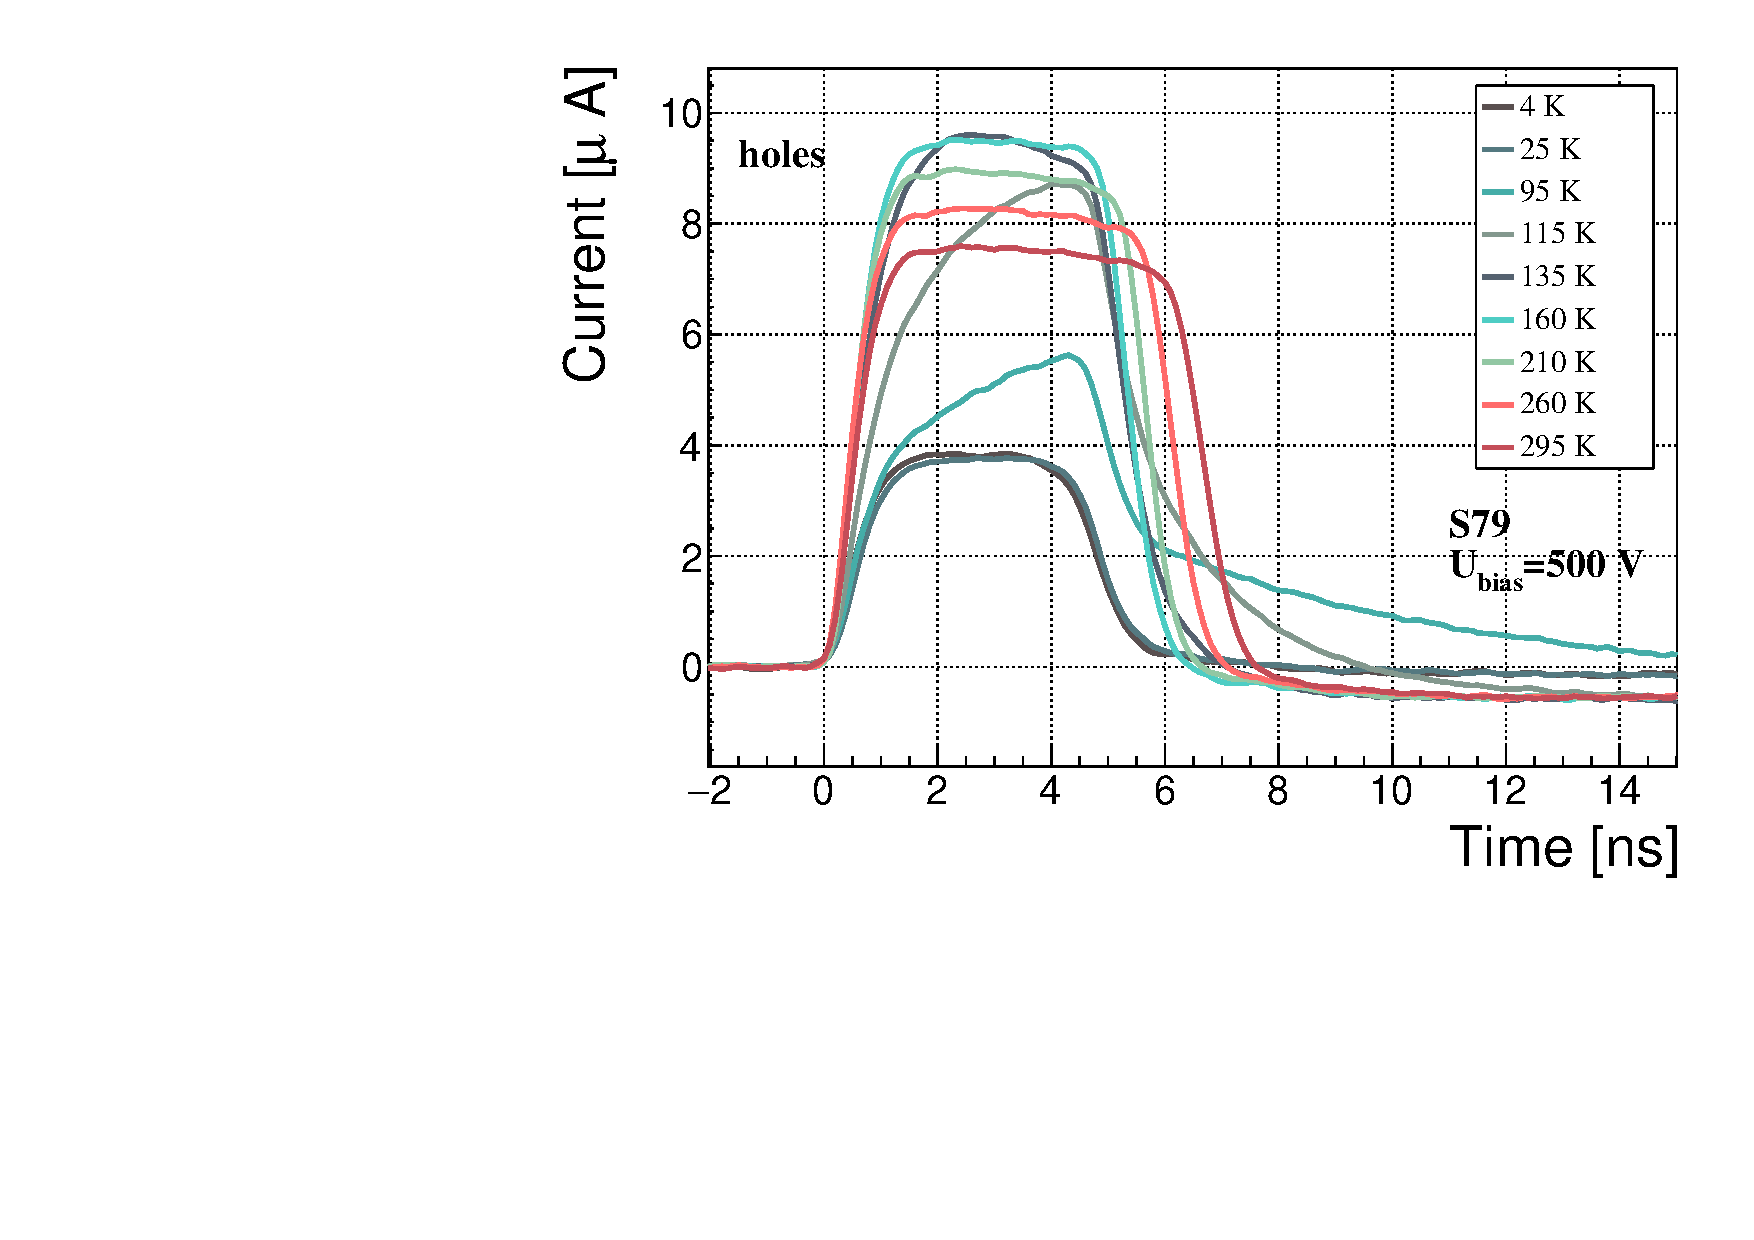
\includegraphics[width=0.47\textwidth]{03_measurement_results/scripts/plots/pulses/S79_holes}  \label{fig:S79minus}} \\
\subfloat{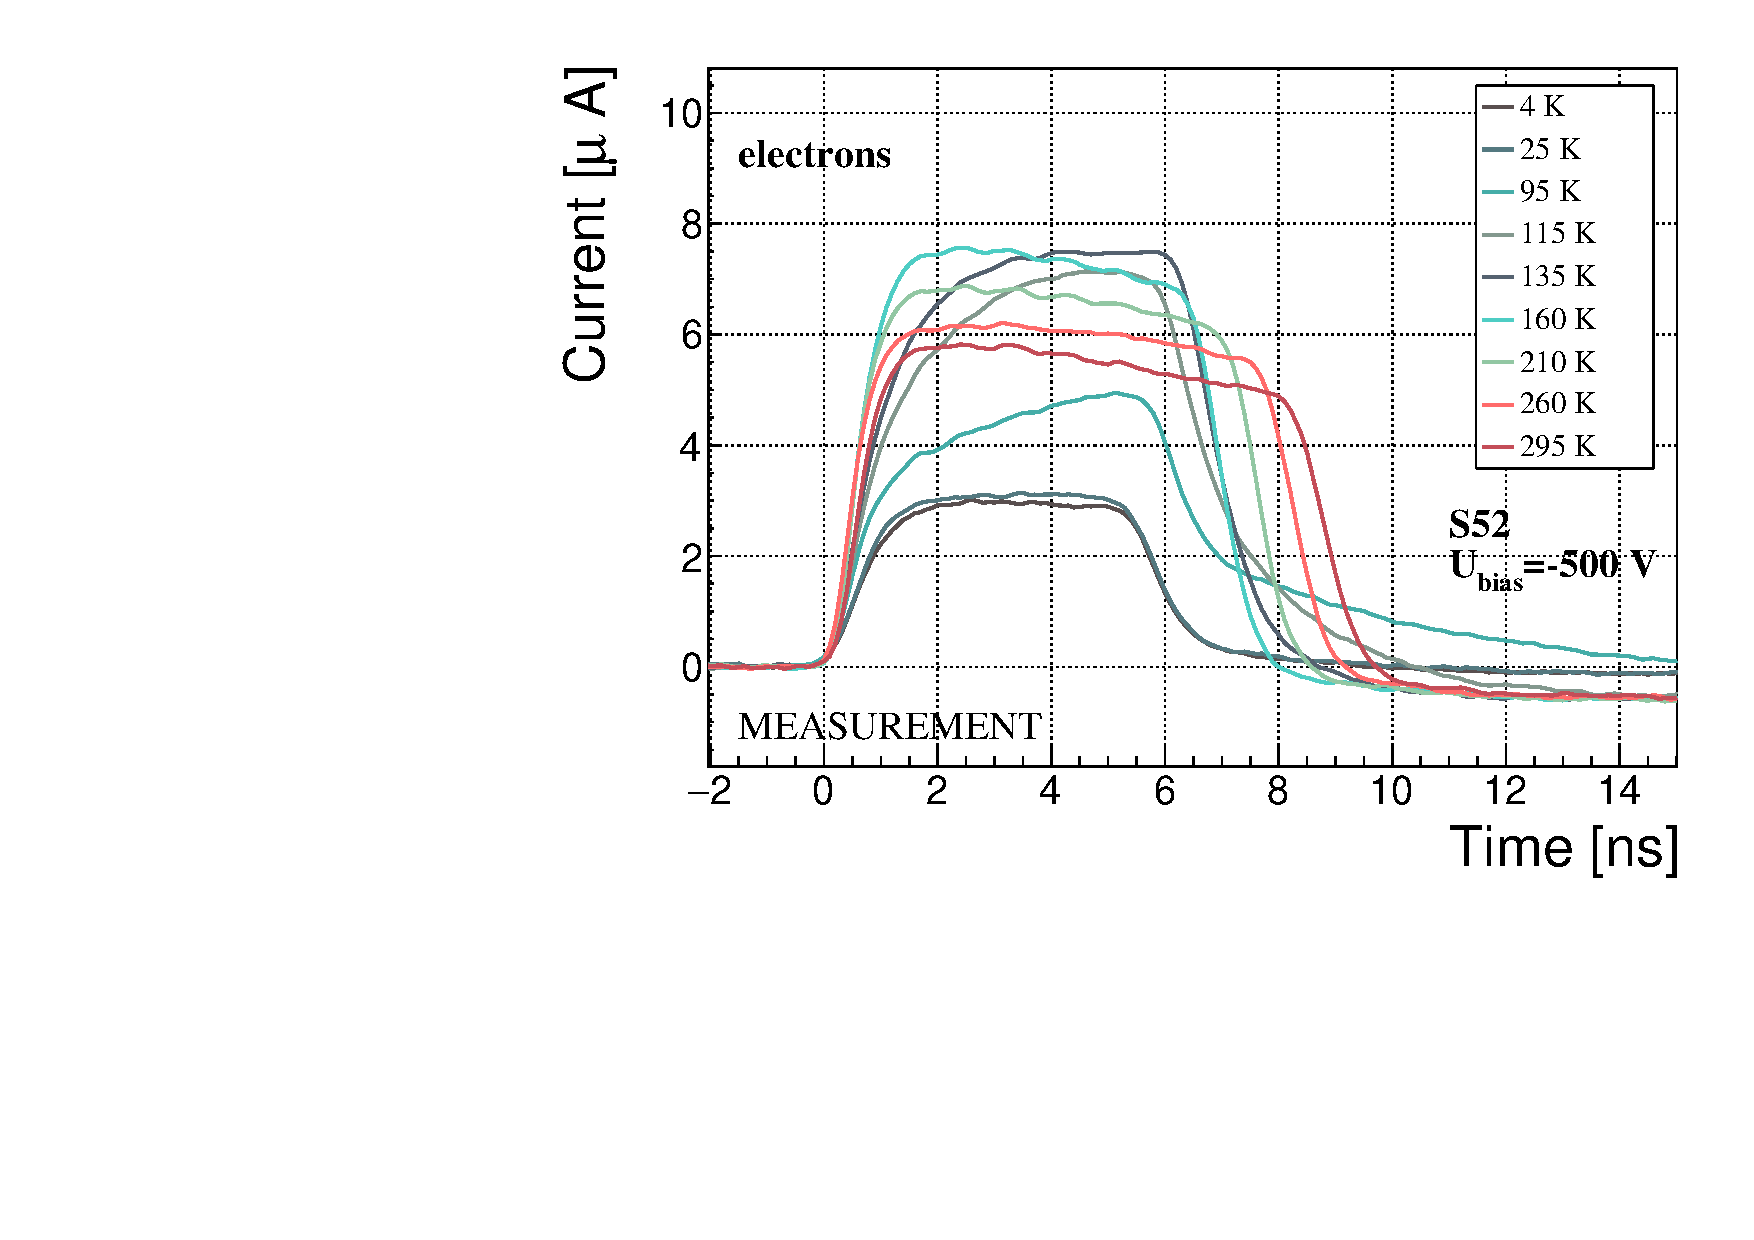
\includegraphics[width=0.47\textwidth]{03_measurement_results/scripts/plots/pulses/S52_elecs} \label{fig:S52plus}} &
\subfloat{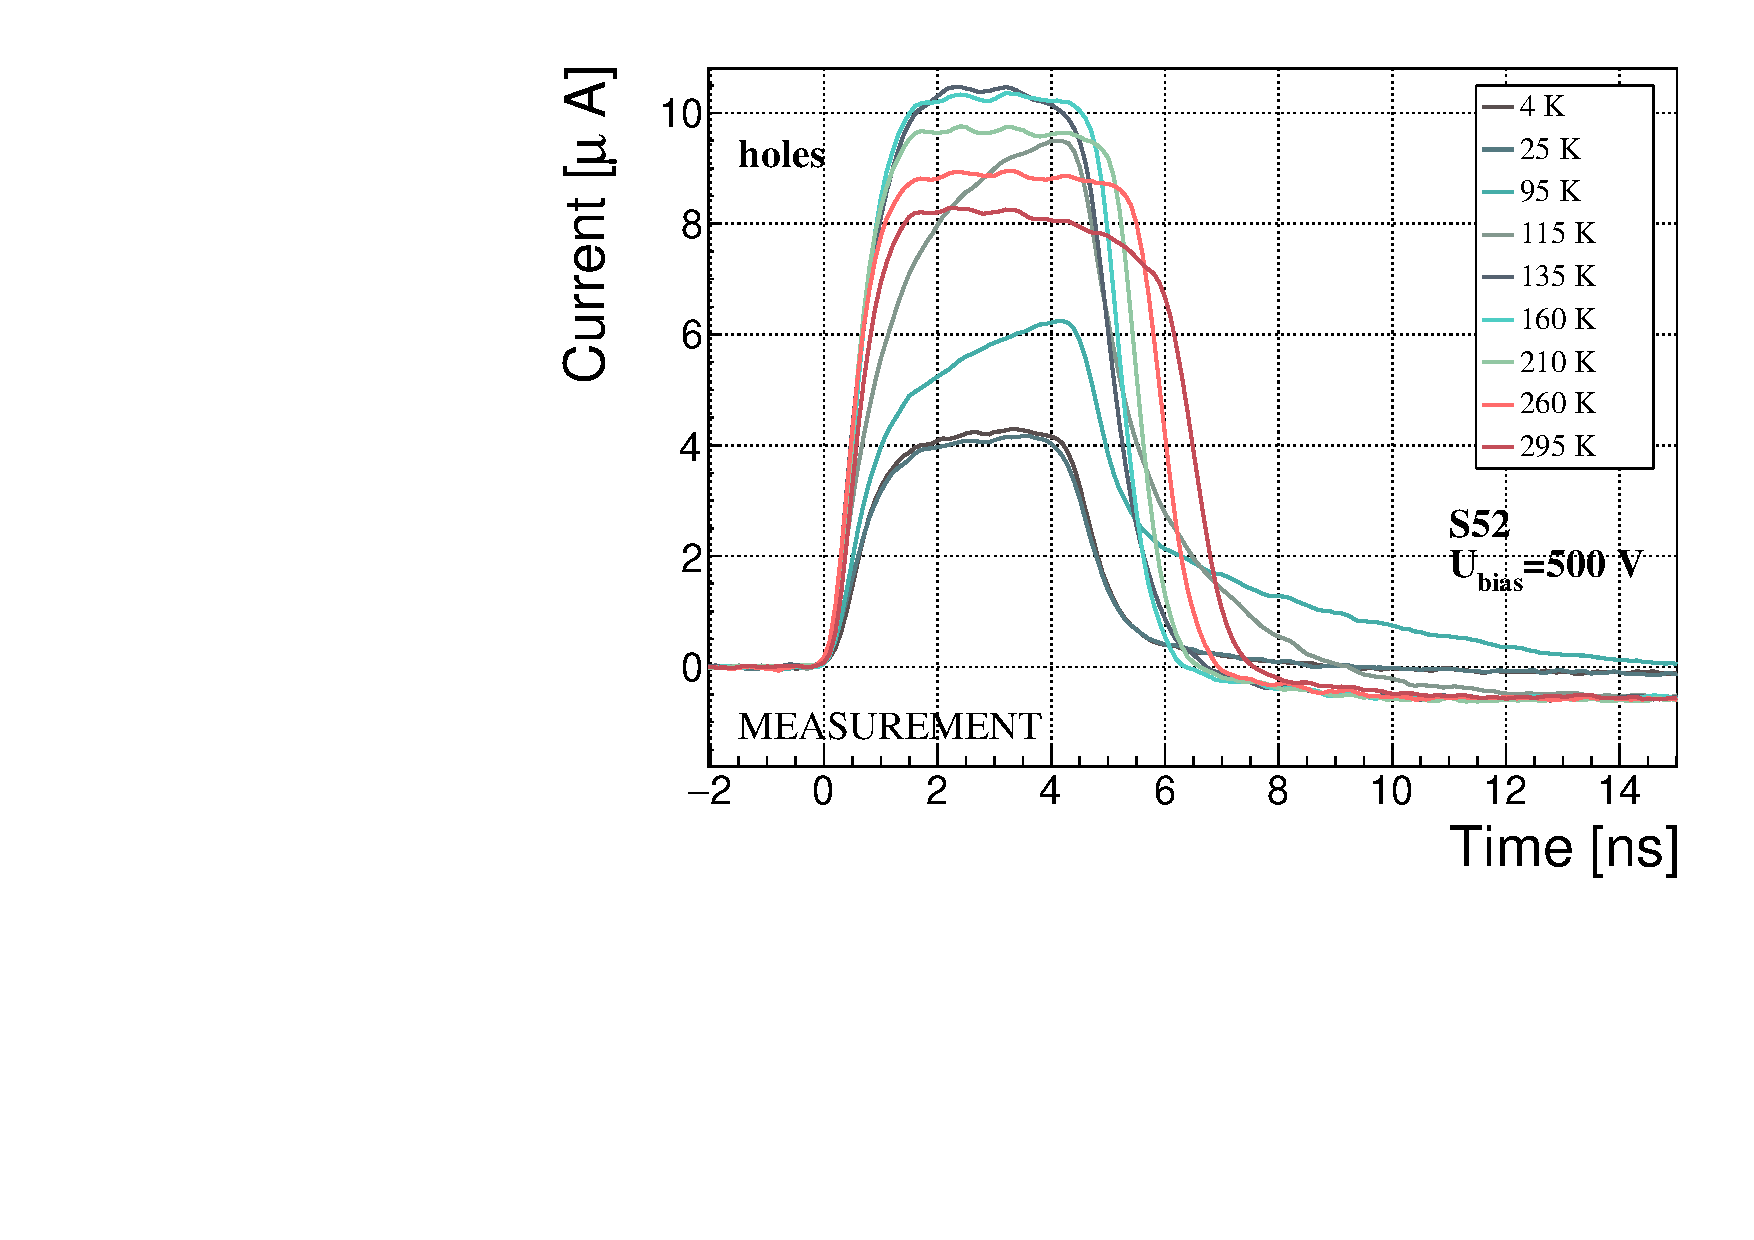
\includegraphics[width=0.47\textwidth]{03_measurement_results/scripts/plots/pulses/S52_holes}  \label{fig:S52minus}}
\end{tabular}
\caption{Three non-irradiated diamond samples: S37, S79 and S52. Several data points between 4~K and 295~K at a bias voltage of $\pm$500~V (electrons and holes). The tilted top of the pulse on the bottom left figure is due to built-up space charge.}
\label{fig:temppulses}
\end{figure}

Figure~\ref{fig:temppulses} shows pulses at a bias voltage set to $\pm500$~V across the range of temperatures between 4~K and 295~K. Several conclusions can be drawn by observing their shape. First, the pulse shapes change with decreasing temperature. The pulse time gets shorter and higher, hinting at the faster carrier drift velocity $v_{\mathrm{drift}}$. Second, between 150~K and 75~K there is a significant change in shape -- the time constant of the rising edge increases significantly and the pulse area decreases~\cite{Jansen:1956431}. From 75~K down to 4~K there is no significant change. Last, the top of the pulse at the S52 is not flat, which means that a portion of the drifting charge is lost along the way. This is due to the built up space-charge, likely by means of crystal defects or impurities introduced during production.

%This could be due to impurities in the diamond bulk, which act as charge traps, or due to the space charge built up in the bulk. A linear pulse top hints on the latter. All in all, the pulse shape changes significantly with temperature, which is predicted by Jansen's model.




% TO-DO Show drift velocity wrt volt
% TO-DO Show drift velocity wrt temp
% TO-DO Show integrated charge
% TO-DO Show Vdrift wrt 1/Voltage
\clearpage
\subsection{Temperature-variant $\upalpha$-TCT after irradiation}
\label{sec:afterirrad}
The irradiated S79 and S52 have been re-tested in the cryostat after irradiation. The aim is to observe how their pulse shapes change with decreasing temperature, in particular the decaying top of the pulses, as shown in figure~\ref{fig:voltpulseAfter}. The decay time gives information on trapping of charge carriers while travelling through the diamond bulk. A variation of the decay time constant as a function of temperature might help to reveal the type and energy level of the charge traps. To observe these effects, a number of requirements have to be met. First, the diamond samples are intentionally not primed prior to the experiment because priming would improve the pulse shapes and change the decay time constant of the signal. Second, keeping in mind that the pulse shape of irradiated diamonds changes with time, the duration of the measurement of an individual data point has to be short -- of the order of 30~seconds. Last, the sequence of the bias voltage settings is important, the reason for which is explained below.
\begin{figure}[!t]
\begin{tabular}{rr}
\subfloat{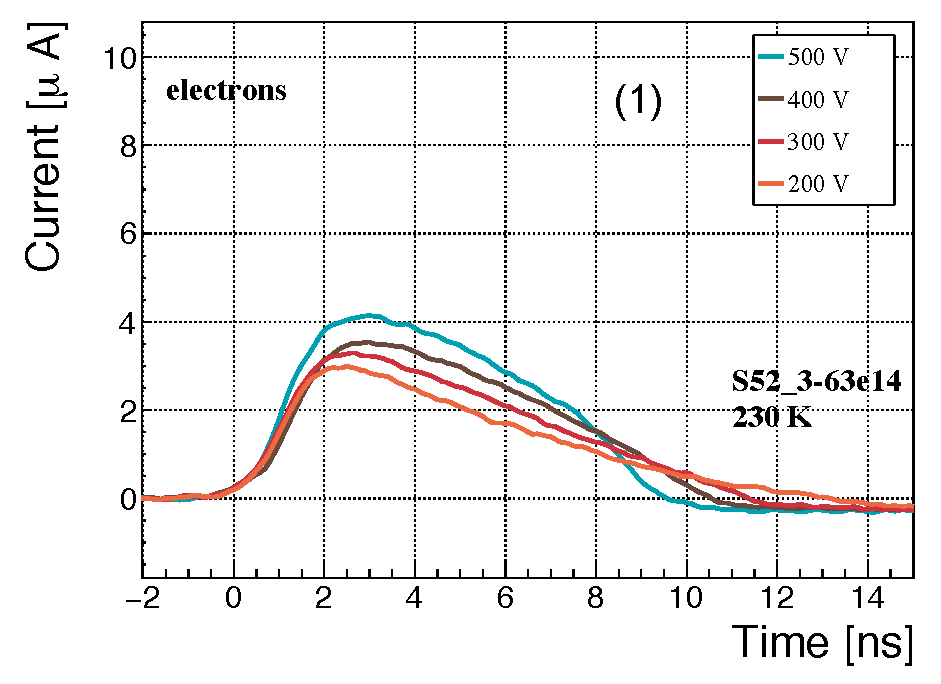
\includegraphics[width=0.47\textwidth]{03_measurement_results/scripts/plots/pulsesVolt/varVolt_S52_3-63e14_elecs_230k_1} \label{fig:S52cTplusAfter230}} &
\subfloat{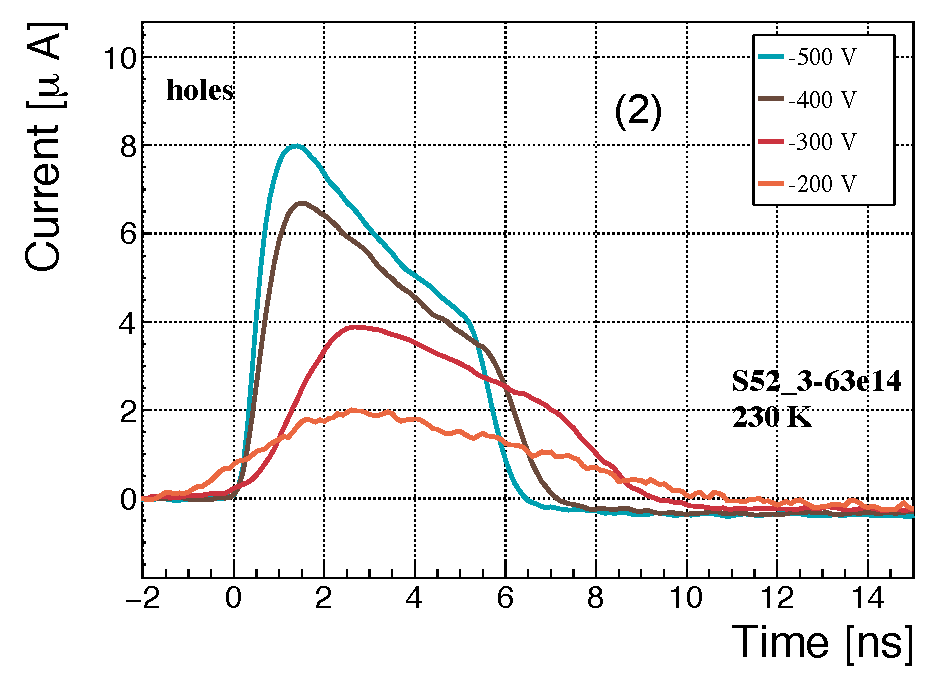
\includegraphics[width=0.47\textwidth]{03_measurement_results/scripts/plots/pulsesVolt/varVolt_S52_3-63e14_holes_230k_1}  \label{fig:S52ctTminusAfter230}} \\
\subfloat{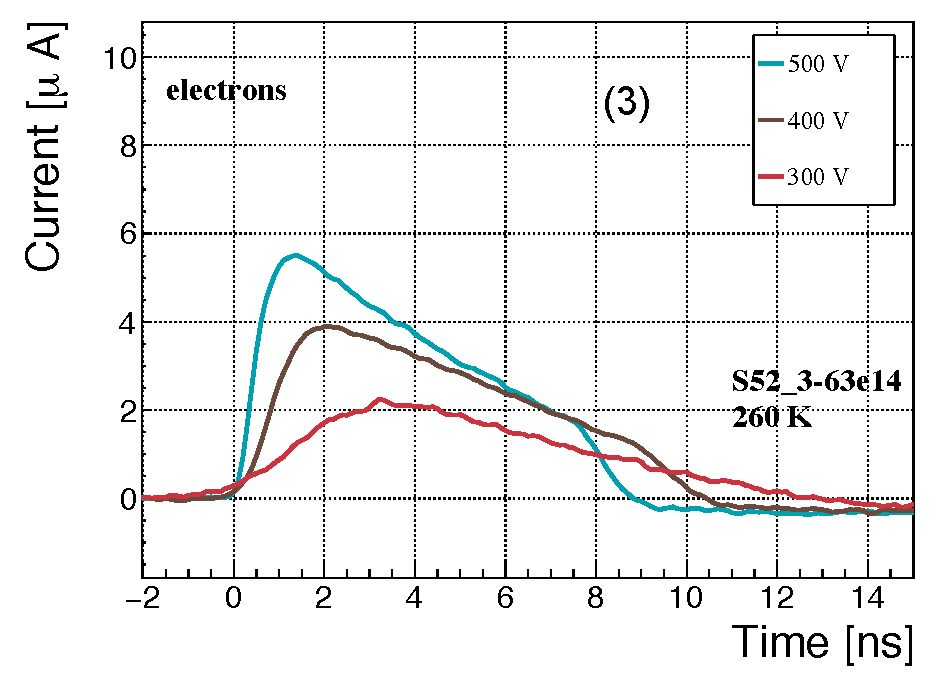
\includegraphics[width=0.47\textwidth]{03_measurement_results/scripts/plots/pulsesVolt/varVolt_S52_3-63e14_elecs_260k_1} \label{fig:S52cTplusAfter260}} &
\subfloat{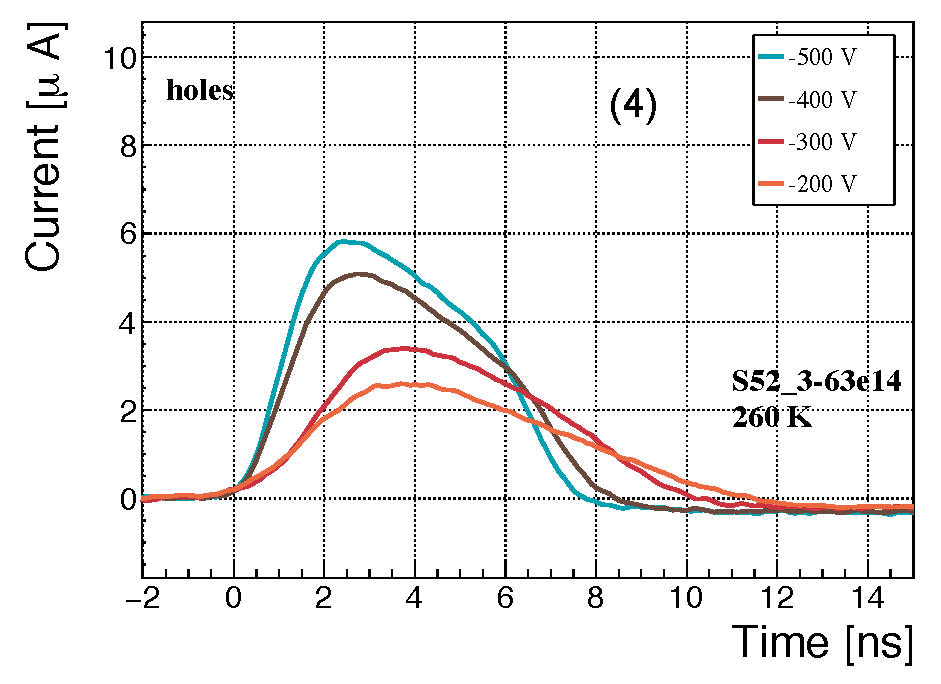
\includegraphics[width=0.47\textwidth]{03_measurement_results/scripts/plots/pulsesVolt/varVolt_S52_3-63e14_holes_260k_1}  \label{fig:S52ctTminusAfter260}}
\end{tabular}
\caption{Varied bias voltage at a fixed temperature for an irradiated sample.}
\label{fig:voltpulseAfter}
\end{figure}
Temporal pulse changes are unavoidable. For instance, one measurement point takes approximately one minute. After the measurement, the bias voltage polarity is swapped for a few seconds to bring the diamond back into its initial state. A few seconds with respect to a minute is not enough, but due to time constraints this cannot be avoided. Therefore when the bias voltage is set to the next value, there is still some residual effect of the previous measurement. Similar to the effects of polarisation, this effect is also decreasing the pulse height. This can be observed in figure~\ref{fig:voltpulseAfter}, which shows the resulting pulses of S52 for bias voltages of $\pm$200~V, $\pm$300~V, $\pm$400~V and $\pm$500~V at 230~K and 260~K. In this case the measurement sequence is: 230K (200~V, 300~V, 400~V, 500~V, -500~V, -400~V, -300~V), 260~K (-200~V, -300~V, -400~V, -500~V, 500~V, 400~V, 300~V). The changes in pulse shapes for holes at 230~K and 260~K cannot be attributed to the temperature change. Instead, the explanation lies in diamond polarisation. This means that, when exposed to an electric field with $\upalpha$ measurements ongoing, an internal electric field of inverse polarity builds up in the diamond, which effectively reduces the overall electric field. This internal field does not dissipate when the external bias voltage is switched off. The diamond becomes polarised. When switching the polarity of the external bias voltage, the internal and external electric field point in the same direction at the beginning, increasing the overall electric field and with it the pulse height. In figure~\ref{fig:voltpulseAfter} this happens when switching from 500~V (figure~\ref{fig:S52cTplusAfter230}) to -500~V (figure~\ref{fig:S52ctTminusAfter230}) at 230~K. The built up polarisation contributes to the pulse having a sharp rising edge and a high amplitude. This effect decays during the next two voltage points. There are a handful of ways to avoid this polarisation effect in the data: 

\begin{enumerate}[itemsep=0.1\baselineskip]
\item After every data point invert the bias voltage and leave it to return to a neutral state for the same amount of time, 
\item Make a hysteresis of data points, going from minimum negative to maximum positive bias several times, 
\item Reduce the measurement time at every bias voltage setting.
\end{enumerate}
Options (1) and (2) are very time consuming and would increase the overall experiment time significantly. The third option would worsen the resulting averaged pulses. Finally an alternative option has been chosen: alternating the starting bias voltage polarity and the sequence of bias voltages at every temperature point. With this option, a minimum systematic error in analysing the pulse shapes is attained.




Figure~\ref{fig:temppulsesAfter} shows the irradiated S52 and S79 as well as the non-irradiated S37 for comparison, all at a bias voltage of $\pm$500~V and at several temperature points between 4~K and 295~K. It is evident that radiation damage affects the shape of the pulses by means of charge trapping across all temperatures. 


\begin{figure}[!t]
\begin{tabular}{rr}
\subfloat{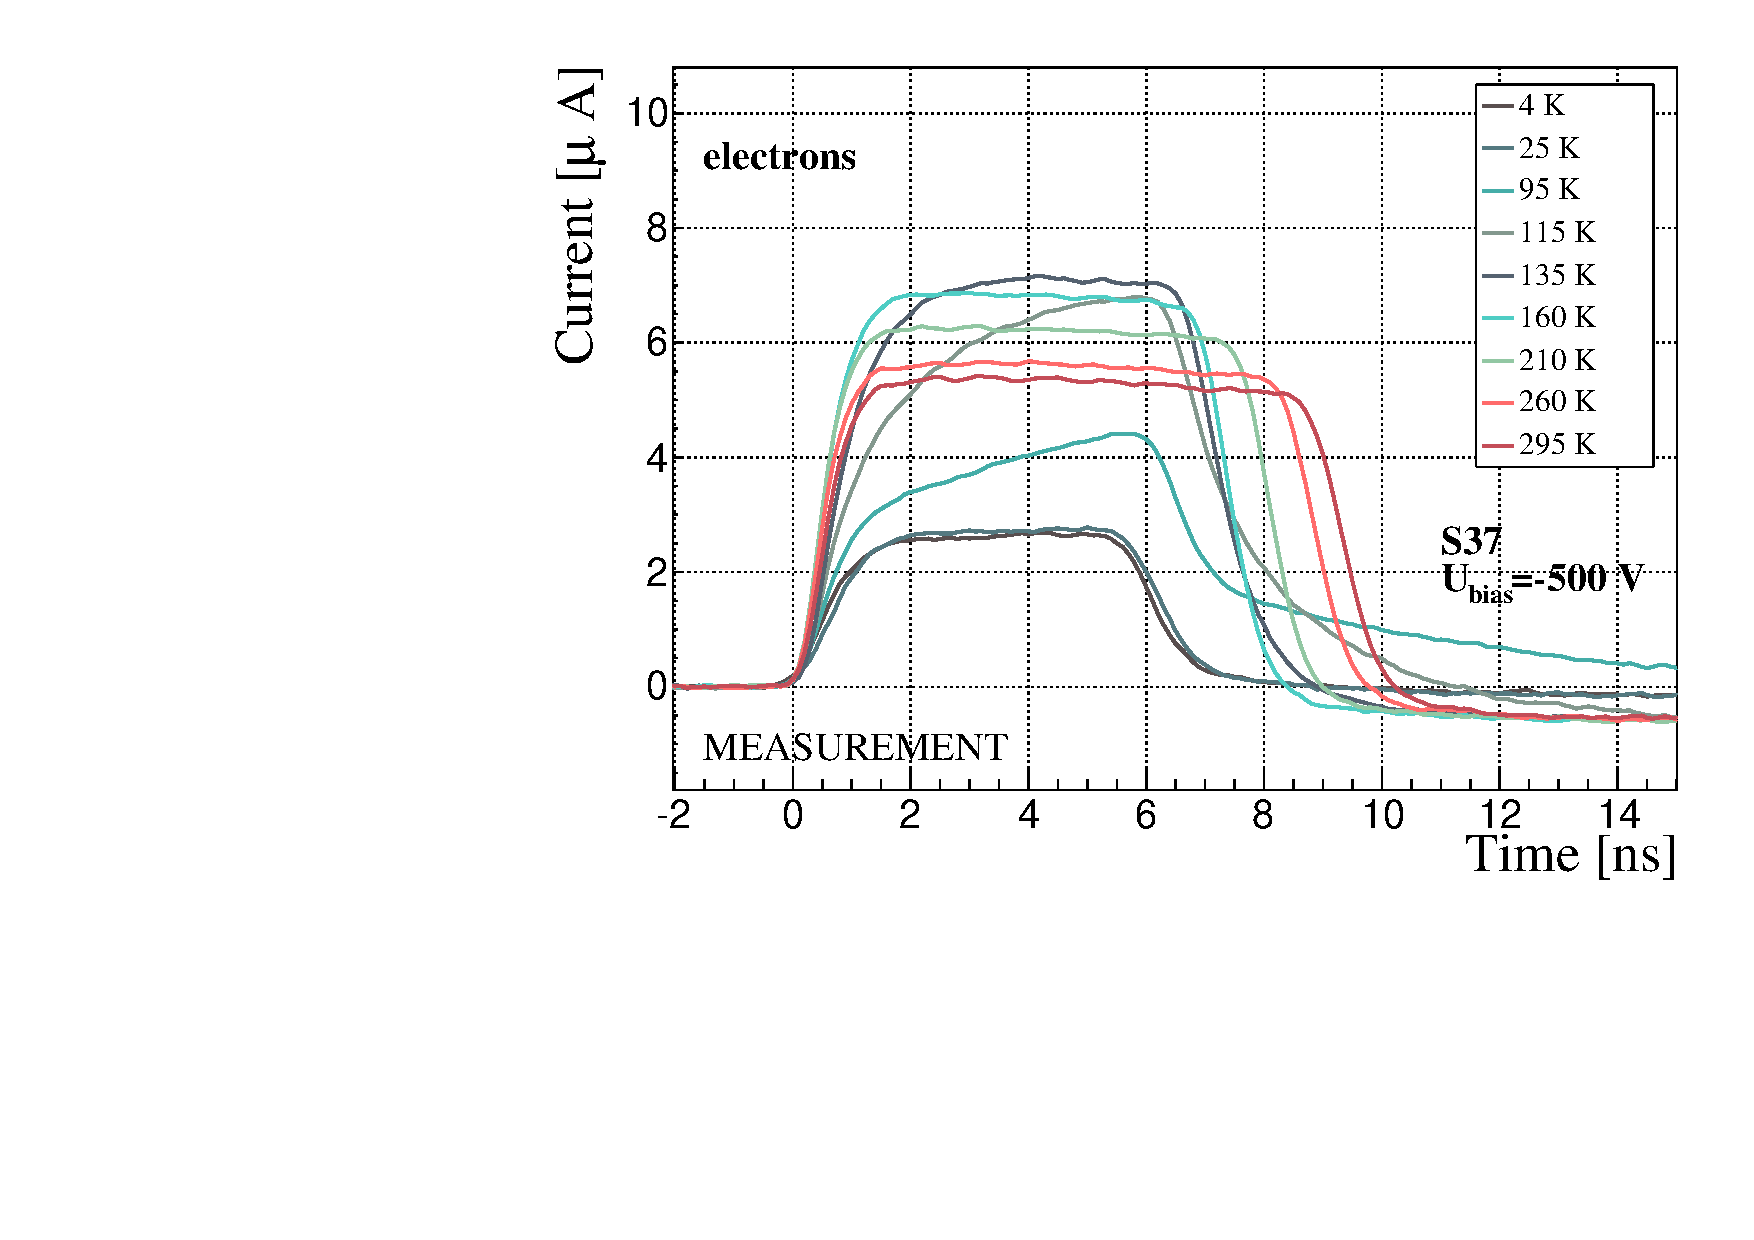
\includegraphics[width=0.47\textwidth]{03_measurement_results/scripts/plots/pulses/S37_elecs} \label{fig:S37plusAfter}} &
\subfloat{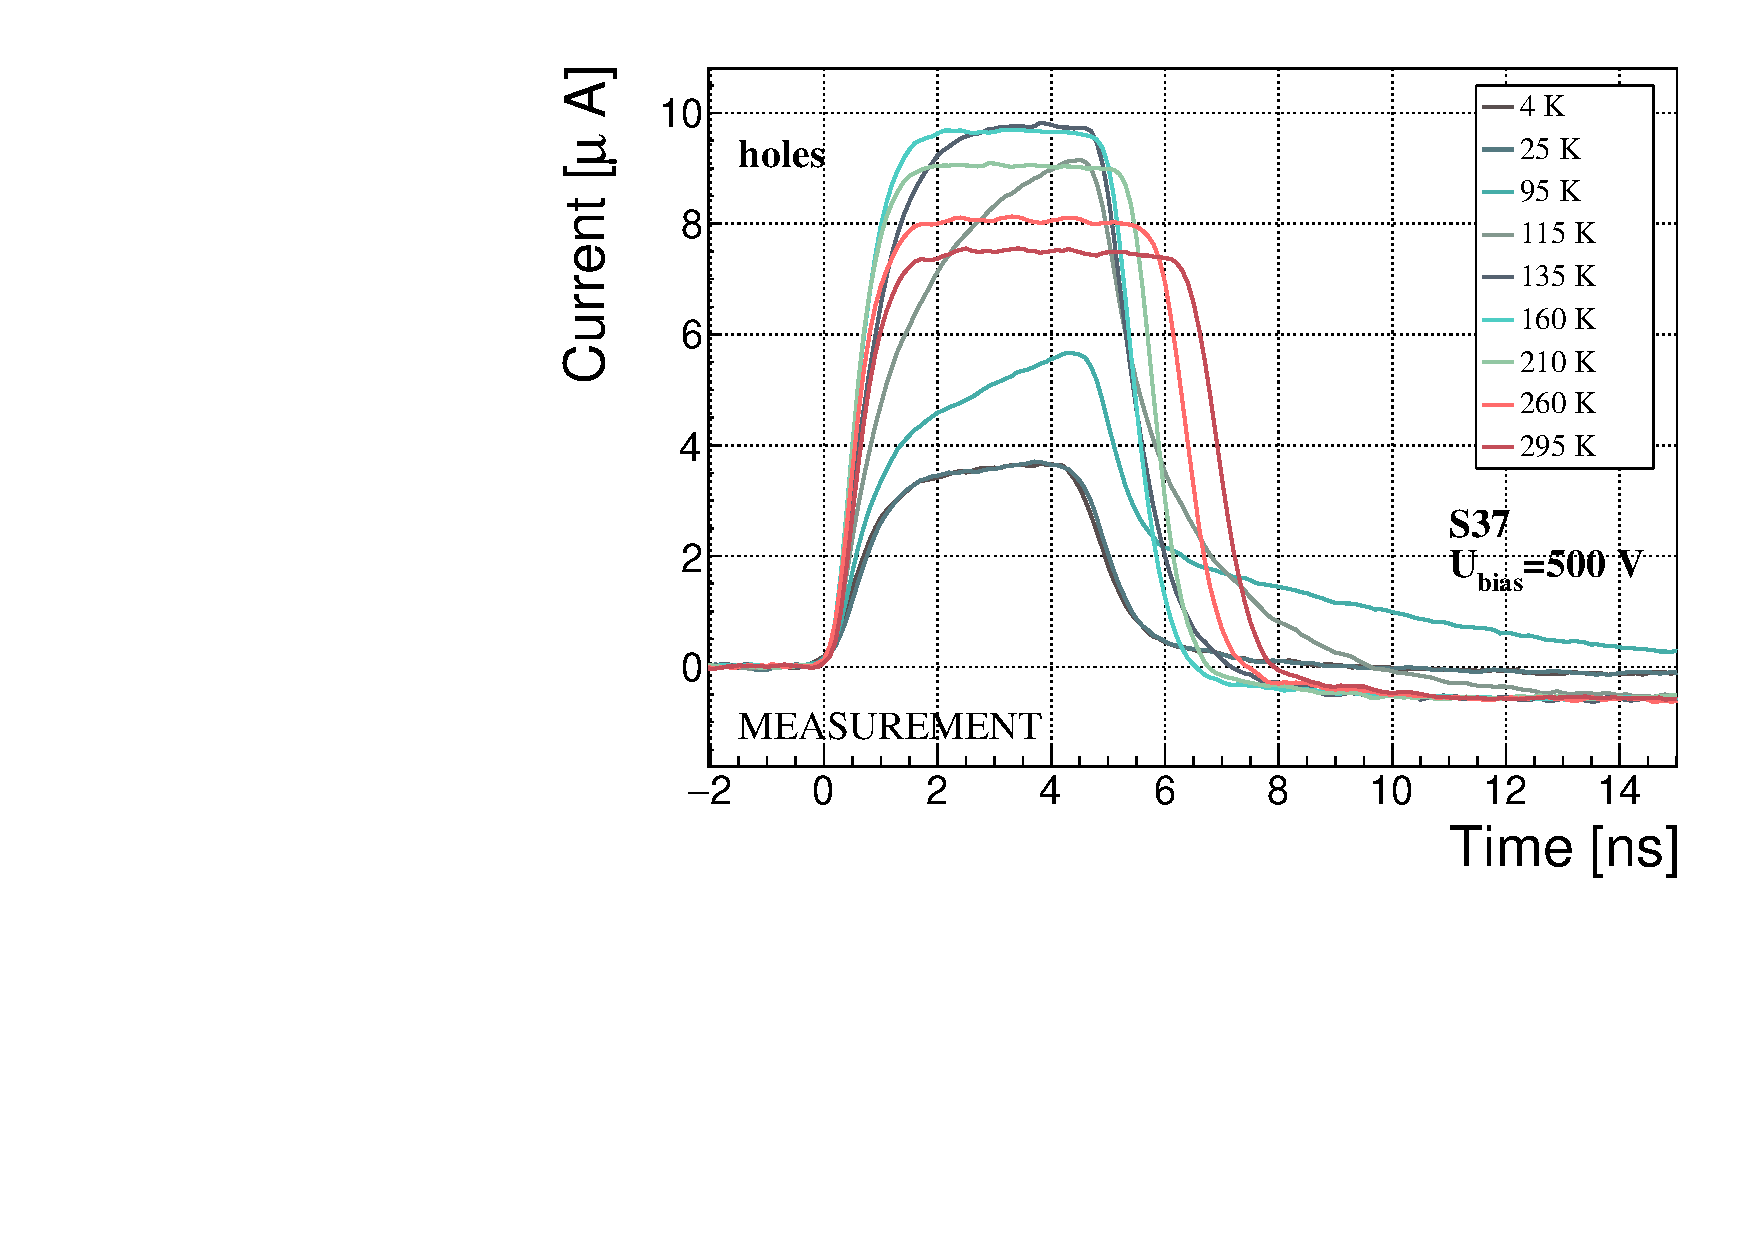
\includegraphics[width=0.47\textwidth]{03_measurement_results/scripts/plots/pulses/S37_holes}  \label{fig:S37minusAfter}} \\
\subfloat{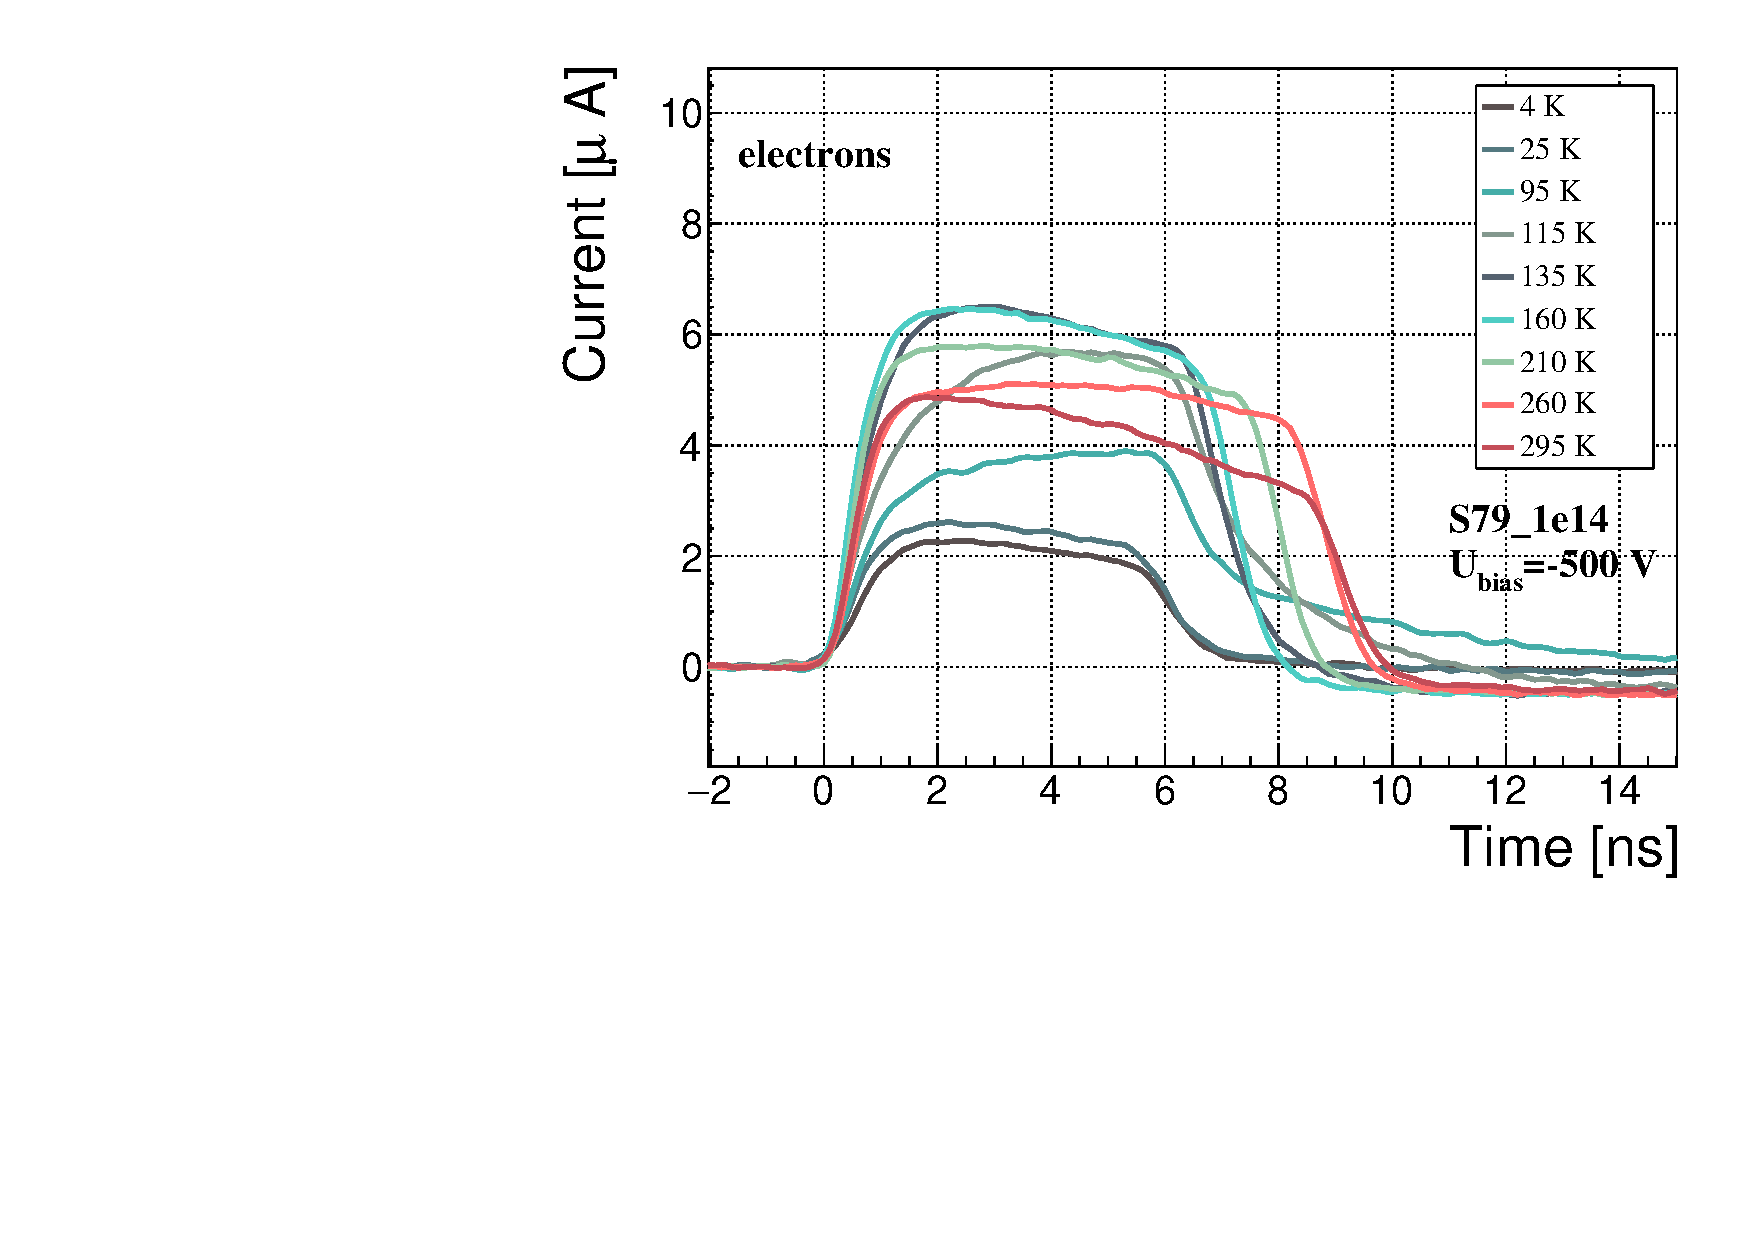
\includegraphics[width=0.47\textwidth]{03_measurement_results/scripts/plots/pulses/S79_1e14_elecs} \label{fig:S79plusAfter}} &
\subfloat{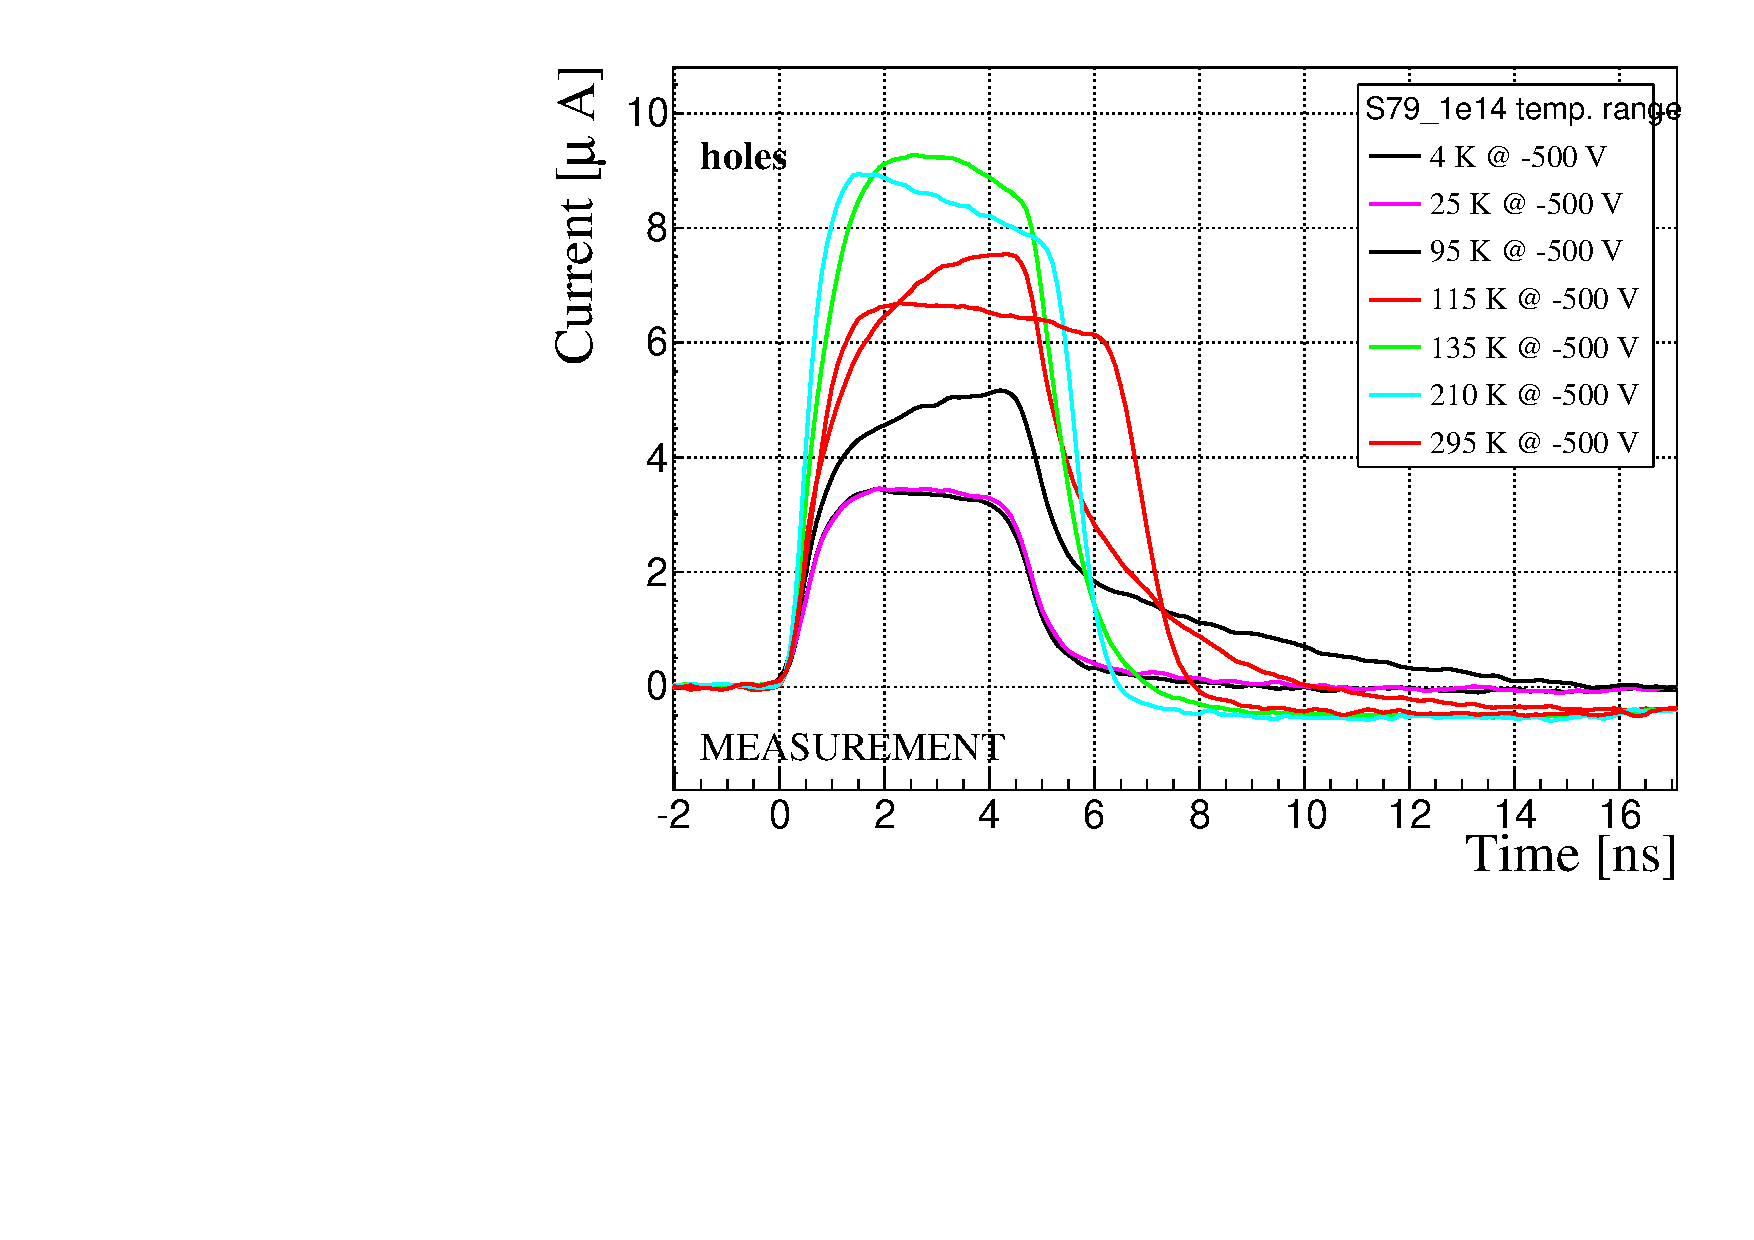
\includegraphics[width=0.47\textwidth]{03_measurement_results/scripts/plots/pulses/S79_1e14_holes}  \label{fig:S79minusAfter}} \\
\subfloat{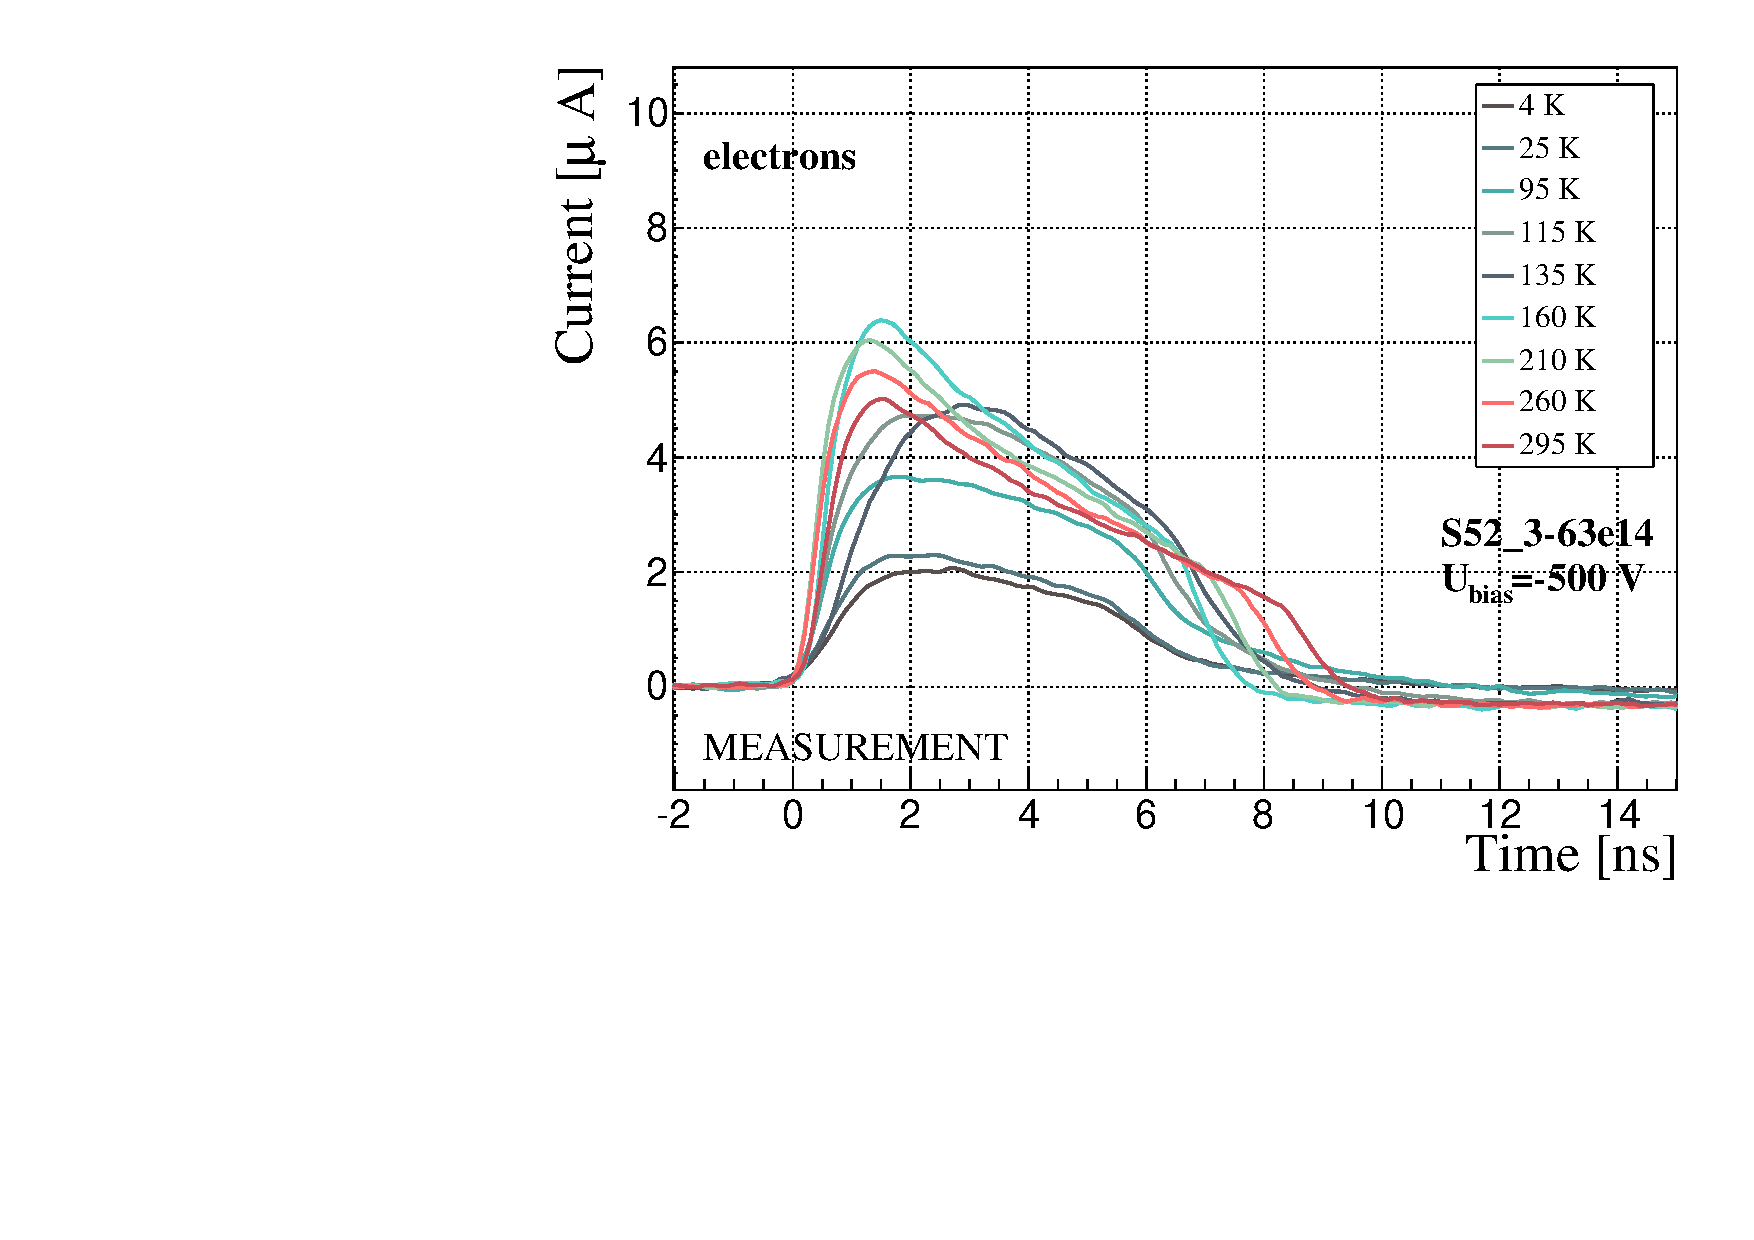
\includegraphics[width=0.47\textwidth]{03_measurement_results/scripts/plots/pulses/S52_3-63e14_elecs} \label{fig:S52plusAfter}} &
\subfloat{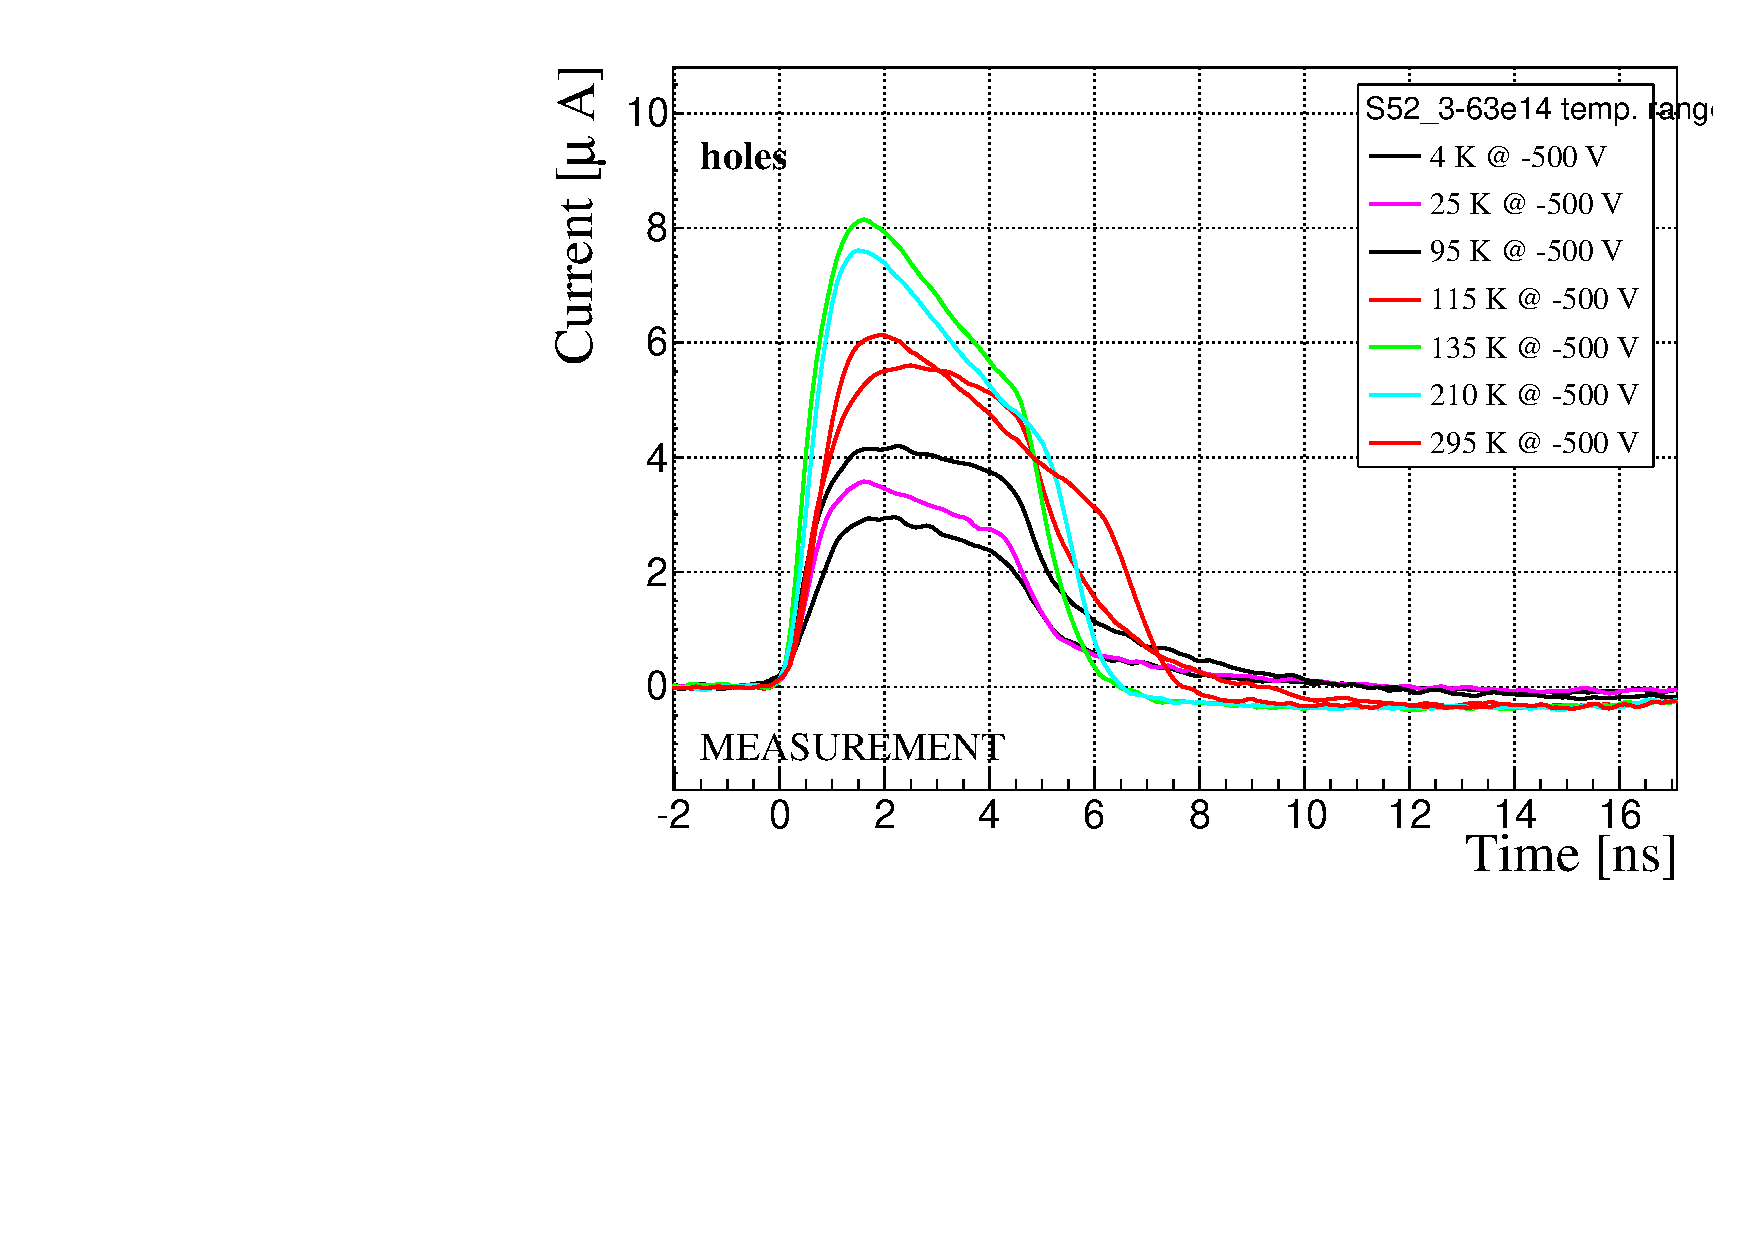
\includegraphics[width=0.47\textwidth]{03_measurement_results/scripts/plots/pulses/S52_3-63e14_holes}  \label{fig:S52minusAfter}}
\end{tabular}
\caption{Non-irradiated S37 and irradiated S79 and S52. Several data points between 4~K and 295~K at a bias voltage of $\pm$500~V.}
\label{fig:temppulsesAfter}
\end{figure}

\clearpage
\subsubsection{Collected charge as a function of temperature}
\label{subsec:qvst}
 The collected charge as a function of temperature for electrons and holes is plotted in figures~\ref{fig:chgtempelecs} and~\ref{fig:chgtempholes}, respectively. The red line shows the results from~\cite{Jansen:1956431}. The new contribution are the data points for the irradiated samples. The focus is on the temperature range between 4--75~K and 150--295~K whereby the creation/decay of excitons is not dominating the pulse shapes.
%  the effect of re-excitation of bound electrons and holes is not prevailing.
%The values for them are lower than the those of non-irradiated samples, which is expected. %TO SUMMARY
\begin{figure}[!t]
\centering
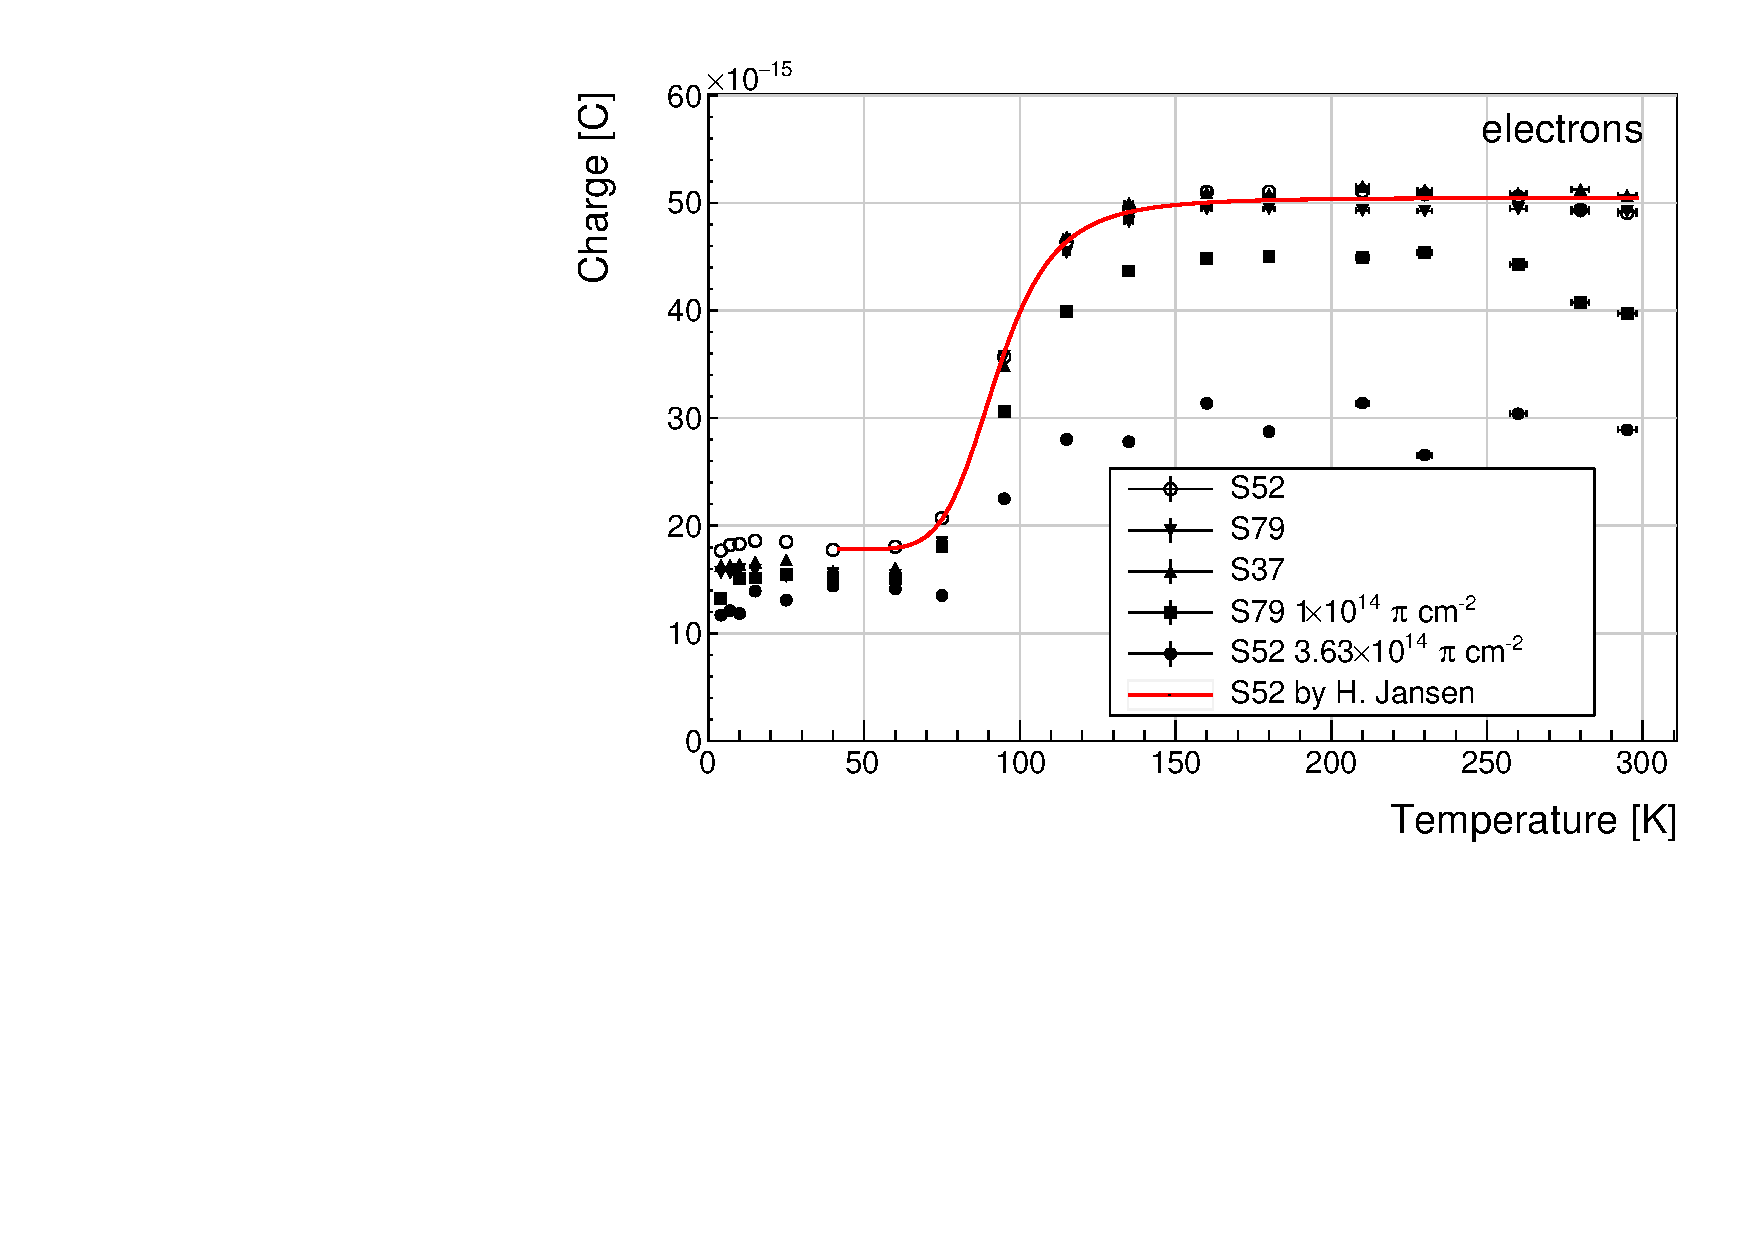
\includegraphics[width=0.70\textwidth]{../scripts/03_experimental_results/plots/charge500V} 
\caption{Collected charge for electrons as a function of temperature.}
\label{fig:chgtempelecs}
\end{figure}
The values for all samples are fairly stable in the range between 4~K and 75~K and between 150~K and 295~K. However, in the values for the irradiated S52 some excursions can be observed. This is due to the sequence of the measurement steps, which results in a hysteresis effect explained in the preceding text.

The collected charge drops significantly from 150~K down to 75~K. In the non-irradiated samples the values in the lower temperature range are approximately 30~\% of those in the high range. For the irradiated samples this difference is lower: 35~\% for S79 and 50~\% for S52.

The highest two temperature points of the S79 are lower due to a change in the measurement setup.

An interesting detail in figure~\ref{fig:chgtempelecs} is that the ratio between the values for non-irradiated samples and their irradiated counterparts at the lower temperature range is different than at the higher range. In other words, the charge loss due to irradiation damage is lower for temperatures between 4~K and 75~K than for temperatures between 150~K and 295~K. The irradiated S52 collects 78~\% of the initial charge in the low temperature range, but only 59~\% of the initial charge for the high range. The values for S79 for these two temperature ranges are 100~\% and 90~\%, meaning that the drop in charge collection efficiency after irradiation to $1\times10^{14}~\uppi$~cm$^{-2}$ is negligible for temperatures below 75~K. To sum up, charge trapping is present in irradiated samples across the entire temperature range, which is evident from the pulse shapes. However, the effect on overall collected charge is reduced for temperatures between 4~K and 75~K.

\begin{figure}[!t]
\centering
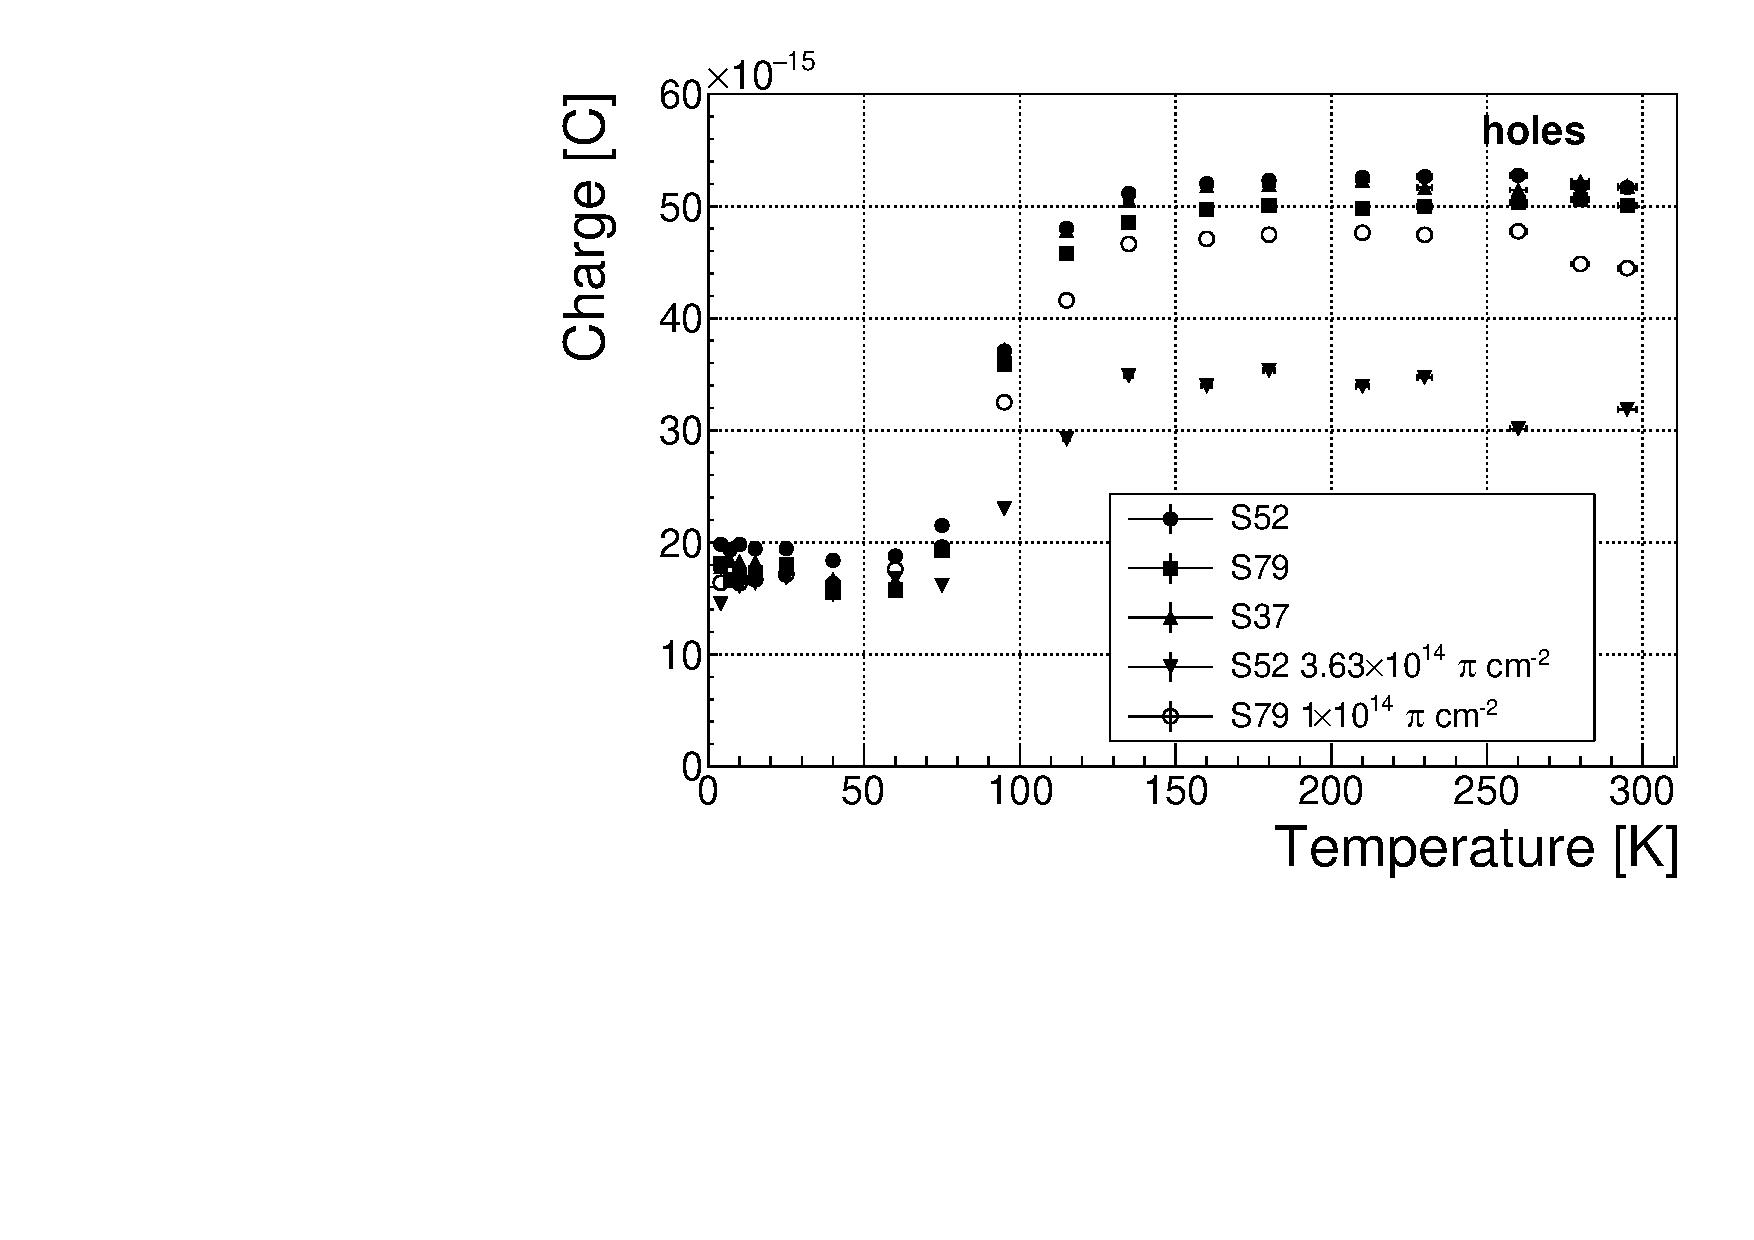
\includegraphics[width=0.70\textwidth]{../scripts/03_experimental_results/plots/charge-500V}
\caption{Collected charge for holes as a function of temperature.}
 \label{fig:chgtempholes}
\end{figure}

\subsubsection{Charge trapping}
A decaying exponential function from equation~\ref{eq:decayexp} has been fitted to the decaying top of the averaged pulses at a bias voltages of $\pm$400~V and $\pm$500~V across all temperatures excluding the transitional range between 75~K and 150~K. The resulting decay time constants $\tau$ are effective carrier trapping times. The values differ for individual temperature points due to changing pulse shapes with time by means of polarisation. This counts as a systematic error. Therefore the fitted $\tau$ for $\pm400$~V and $\pm500$~V are averaged into one value representing the measurement at that temperature point. The time constants should be infinite for an ideal and non-irradiated sample. %Here a slightly tilted top of the pulse due to space-charge is already successfully fitted with an exponential function (a pitfall in the automatic analysis), resulting in a $\tau$ of the order of (200$\pm$20)$\times10^{-9}$~s. Consequently the fitting method is not adequate for non-irradiated samples. 

As seen in figures~\ref{fig:lifetimevstempE} and ~\ref{fig:lifetimevstempH}, the fitted values of the irradiated samples are fairly stable across all temperatures. There is a slight increase in the decay time constant of the S52 from $(6.0\pm0.5)\times10^{-9}$~s above 150~K to ($8.5\pm0.9$)$\times10^{-9}$~s below 75~K. This step is however not observable in the S79 data. With only one sample exhibiting this behaviour, the effect is not significant. Judging by the data acquired, the samples would need to be irradiated to doses above $5\times10^{14}~\uppi~$cm$^{-2}$ to quantify this effect in detail. Building on this assumption, the conclusion is that the signal decay time constant for irradiated sCVD diamond is constant across the temperature range between 4~K and 295~K, excluding the transitional range between 75~K and 150~K  where it cannot be quantified properly. All things considered, the values can be averaged into one single effective trapping time value for electrons and one for holes for further analysis. 
\begin{figure}[!t]
%\centering
\begin{tabular}{cccc}
\subfloat{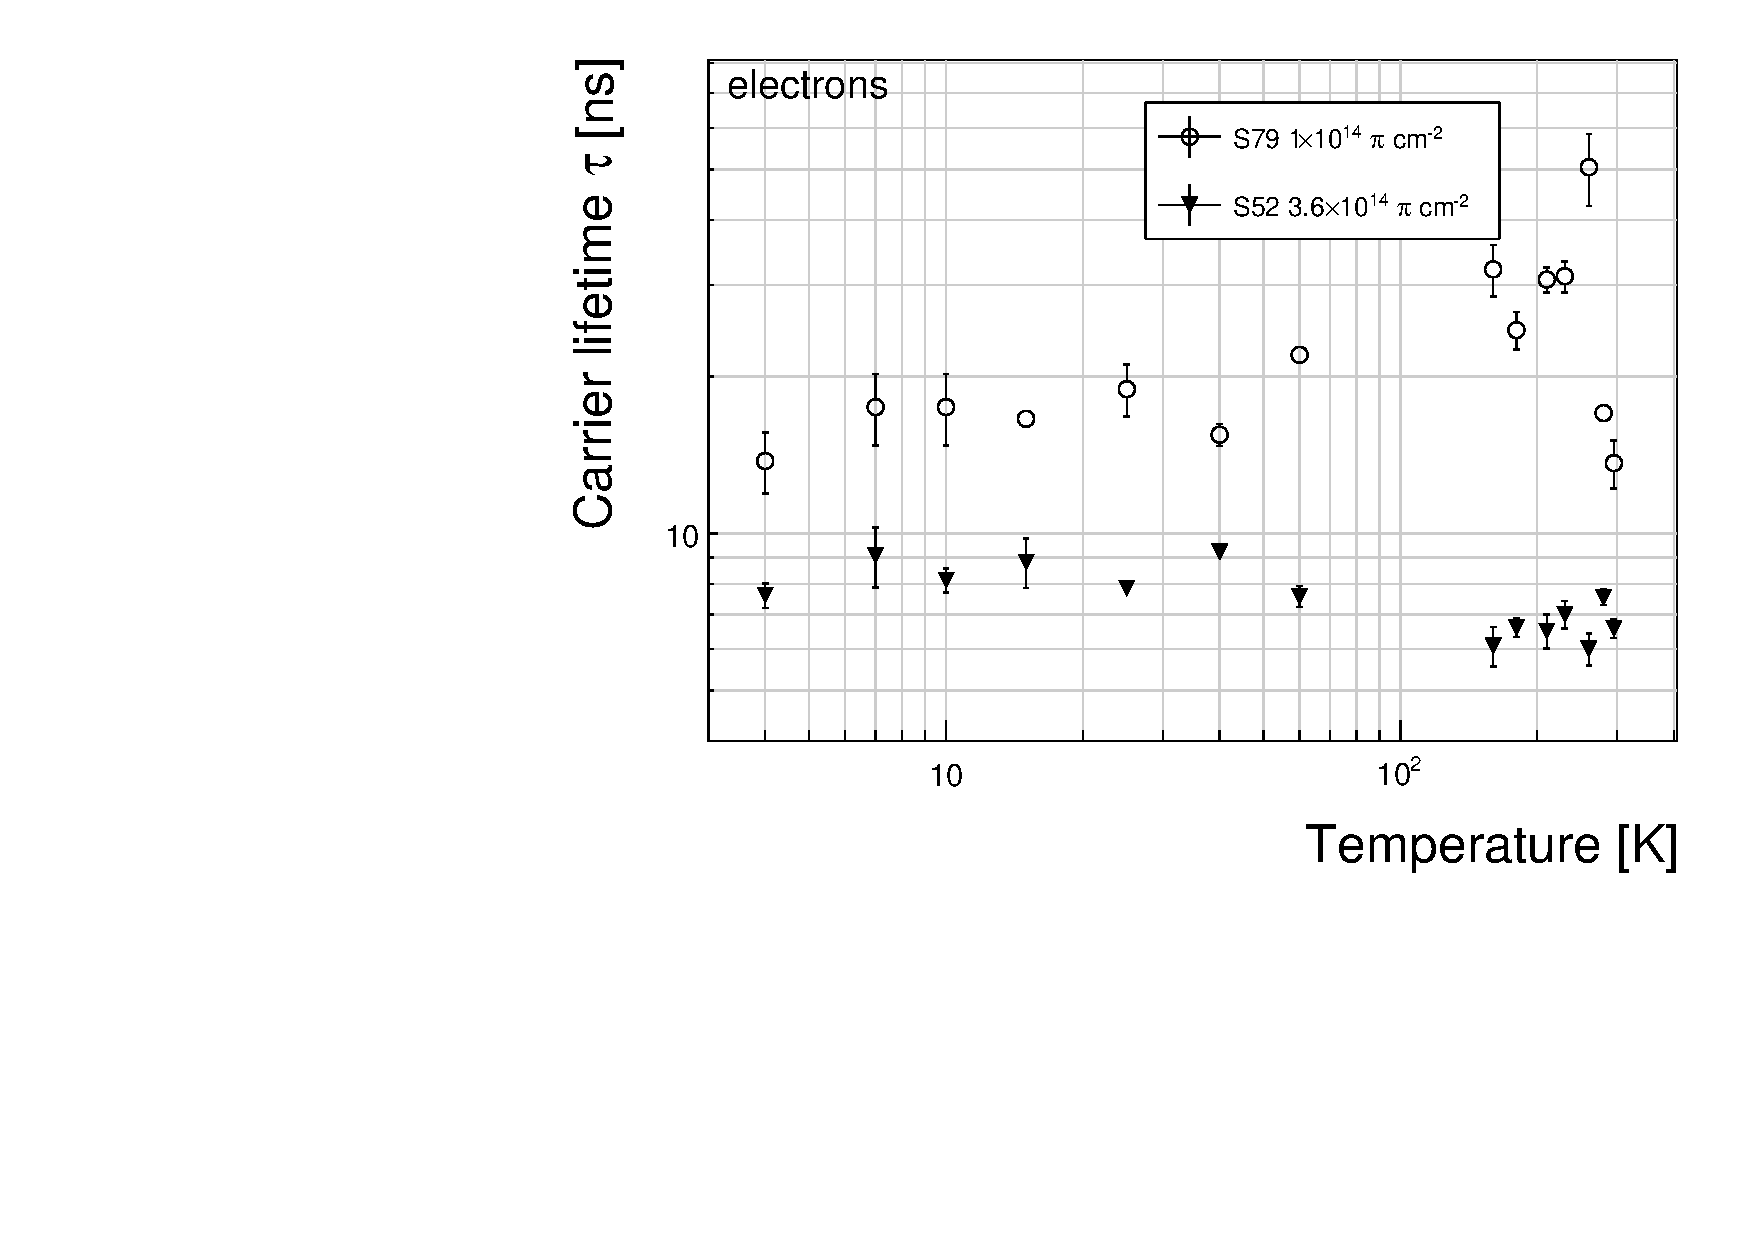
\includegraphics[width=0.47\textwidth]{03_measurement_results/scripts/plots/taunew/lifetimevstempE} \label{fig:lifetimevstempE}} &
\subfloat{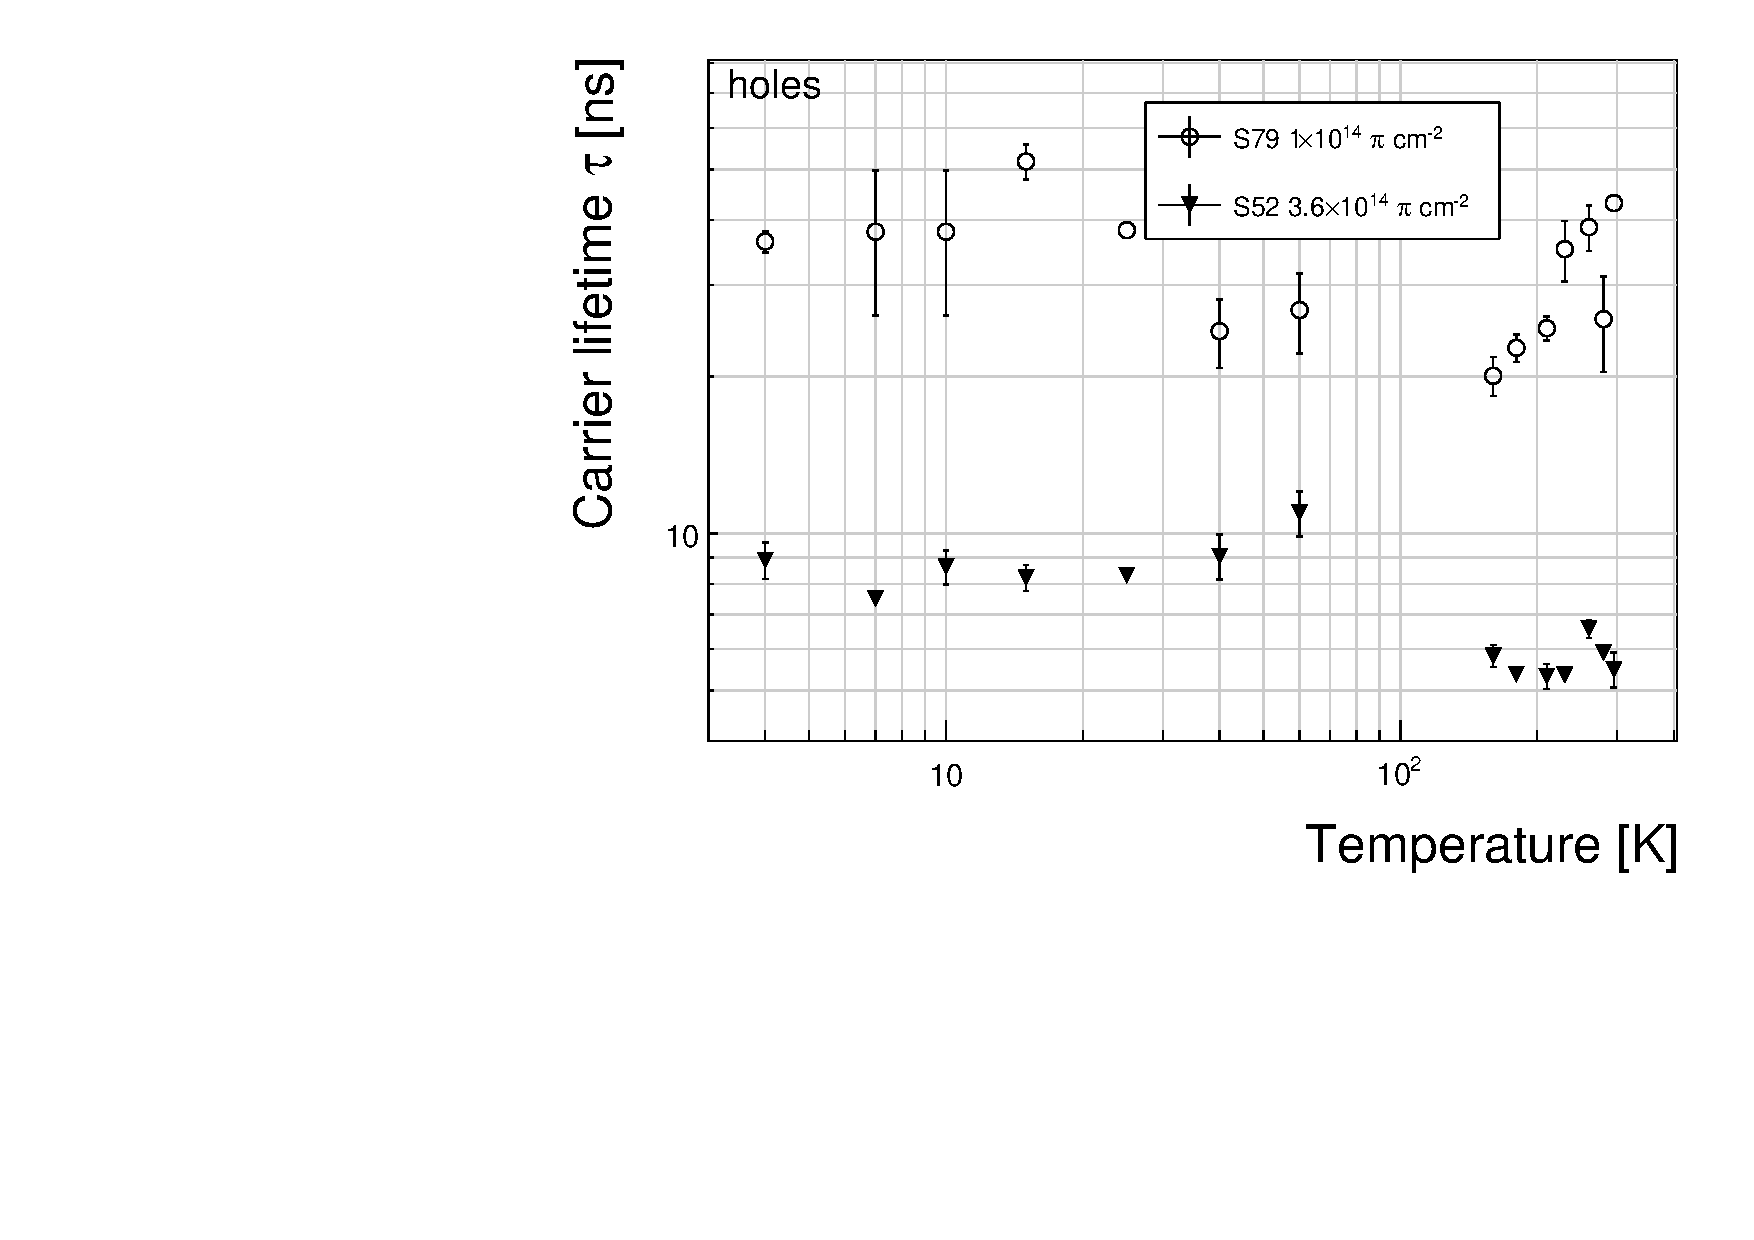
\includegraphics[width=0.47\textwidth]{03_measurement_results/scripts/plots/taunew/lifetimevstempH}  \label{fig:lifetimevstempH}}
\end{tabular}
\caption{Charge carrier lifetime as a function of temperature for electrons and holes at $\pm$400~V and $\pm$500~V. The data points between 75~K and 150~K are omitted.}
\end{figure}
The effective trapping time is inversely proportional to the fluence~\cite{Bates2005113}:
\begin{equation}
\label{eq:ltfactor}
\frac{1}{\tau} = \beta\cdot\Phi
\end{equation} 
where $\beta$ is the proportionality factor. A low $\beta$ value would mean that the trapping centres in the sensor are created with a low rate. Figure~\ref{fig:lifetimevsdose} shows the inverse trapping times of the non-primed irradiated samples as a function of $\uppi_\mathrm{300~MeV}$ fluence. $\beta$ is the slope of the fitted linear function. The fitted factors are $\beta_\mathrm{e}=(3.8\pm0.9)\times10^{-16}~$cm$^2$/ns and $\beta_\mathrm{h}=(3.4\pm0.8)\times10^{-16}~$cm$^2$/ns. Comparing to silicon detectors in~\cite{Bates2005113}, the value for the sCVD diamond is two times lower, meaning that it takes twice as much irradiation to create the same amount of charge traps in diamond than in silicon.

 


\begin{figure}[!t]
\centering
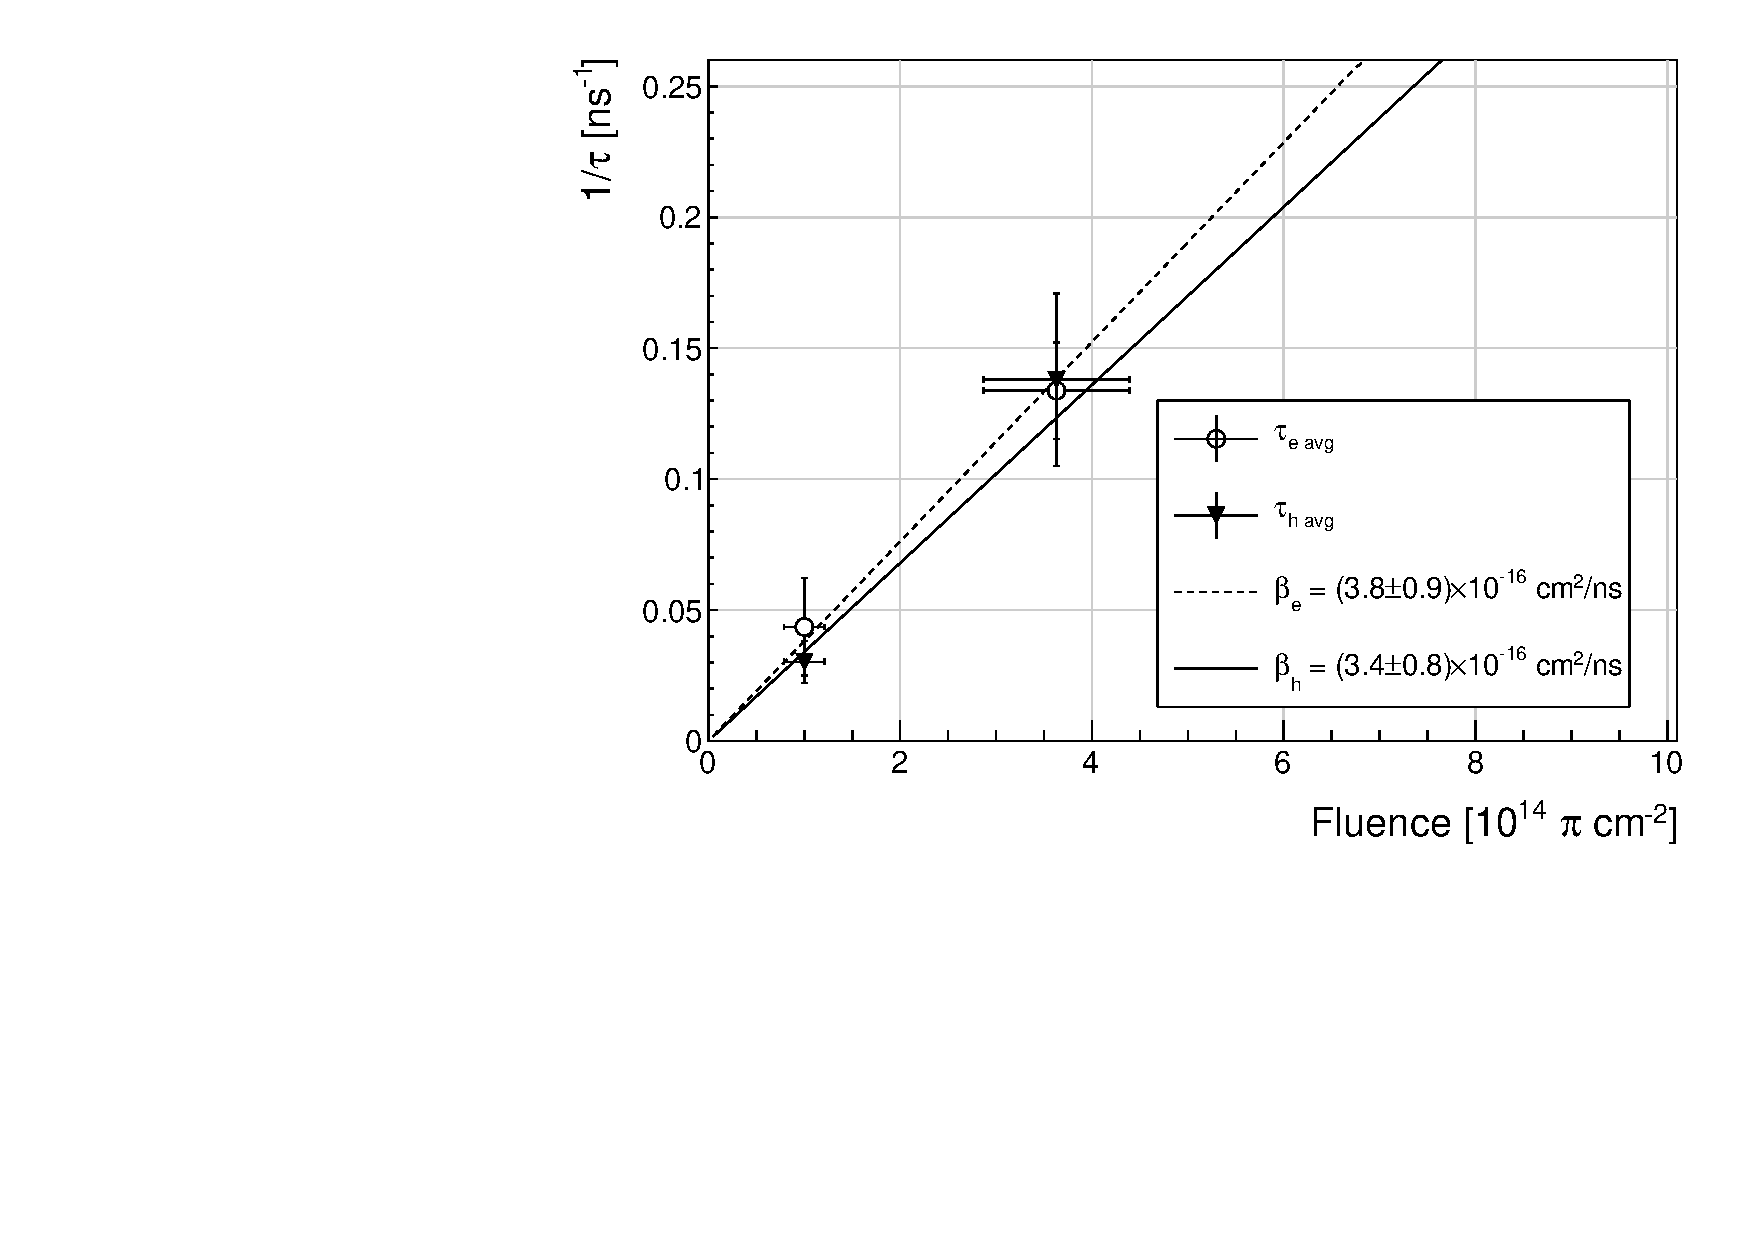
\includegraphics[width=0.7\textwidth]{03_measurement_results/scripts/plots/taunew/avglifetime1} 
\caption{This figure shows the inverse charge trapping times averaged over all temperatures and plotted as a function of the $\uppi$ fluence.}
\label{fig:lifetimevsdose}
\end{figure}








% ---------------------------------------------------------------------------------------------------------------
\clearpage
\section{Conclusion}
\label{sec:radlimit}
% ---------------------------------------------------------------------------------------------------------------
This chapter gives an overview of the capabilities and limitations of diamond as a particle detector. Two effects on diamond are studied -- radiation and temperature. 

Two sCVD diamond detectors were irradiated with 300~MeV pions. They were tested alongside a non-irradiated sample to observe the changes in the ability to detect $\upalpha$, $\upbeta$ and $\upgamma$ radiation. Their charge collection efficiency was measured in a test beam facility. The results were compared to the results from the RD42 collaboration and a DPA model. A radiation damage factor $k_{\mathrm{\lambda}}=(4.4\pm1.2)\times10^{-18}~\upmu$m$^{-1}$~cm$^{2}$ was obtained for $\uppi_{\mathrm{300~MeV}}$ particles. The data point was not in agreement with the data provided by RD42 nor with the model. %However, the irradiation process and the low number of tested samples hold a relatively high statistical uncertainty. 
Most likely this is because there was no diamond surface treatment done in between the measurements, as is the case in the study conducted by RD42. The results obtained in the course of these measurements are going to be fed into the existing pool of data in the RD42 collaboration.

The next step was to test the long-term capabilities for $\upalpha$ detection. The shape of the ionisation profile was investigated to determine the behaviour of the charge carriers in the irradiated diamond. An exponential decay was observed in the pulses of irradiated samples, proving that there are charge traps in the bulk that were created during irradiation. Then a long-term stability test was carried out. The results show that the irradiated diamond detectors do not provide a stable and reliable long-term measurement of $\upalpha$ particles. This might be due to a space-charge build-up in the bulk, which changes the electric field, affecting the charge carriers. A procedure to improve the pulse shape using $\upbeta$ and $\upgamma$ radiation was proposed.

Finally, the diamond sensors were cooled down to temperatures between 4~K and 295~K. Their response to $\upalpha$ particles was observed. The results of the non-irradiated and irradiated samples were compared. The effect of reduction for the number of drifting charges due to exciton creation was observed in both sets of data. The second set had a superimposed effect of charge trapping during the drift, which was represented by an exponential decay in the signal. The decay time constant did not change with temperature. Therefore all temperature points for individual samples were averaged and the decay time constants were plotted as a function of fluence. Proportionality factors for defect production rate $\beta_\mathrm{e}=(3.8\pm0.9)\times10^{-16}$~cm$^2$/ns and $\beta_\mathrm{h}=(3.4\pm0.8)\times10^{-16}$~cm$^2$/ns for non-primed diamonds were extracted.
